\documentclass[
  bibliography=totoc,     % Literatur im Inhaltsverzeichnis
  captions=tableheading,  % Tabellenüberschriften
  titlepage=firstiscover, % Titelseite ist Deckblatt
]{scrartcl}

% Paket float verbessern
\usepackage{scrhack}

% Seitenränder etc.
\usepackage[a4paper]{geometry}

% Warnung, falls nochmal kompiliert werden muss
\usepackage[aux]{rerunfilecheck}

% deutsche Spracheinstellungen
\usepackage{polyglossia}
\setmainlanguage{german}

%\usepackage{sourceserifpro}
%\usepackage{sourcesanspro}
%\usepackage{charter}
%\usepackage{mathpazo}

% unverzichtbare Mathe-Befehle
\usepackage{amsmath}
% viele Mathe-Symbole
\usepackage{amssymb}
% Erweiterungen für amsmath
\usepackage{mathtools}

\ExplSyntaxOn
\NewDocumentCommand{\kf}{}{
\begin{align}
    \Aboxed{k\text{-Form} \ \hat= \ \text{Kuchenform}} \\
\end{align}
}
\ExplSyntaxOff

% Fonteinstellungen
\usepackage{fontspec}
% Latin Modern Fonts werden automatisch geladen

\usepackage[
  math-style=ISO,    % ┐
  bold-style=ISO,    % │
  sans-style=italic, % │ ISO-Standard folgen
  nabla=upright,     % │
  partial=upright,   % ┘
  warnings-off={           % ┐
    mathtools-colon,       % │ unnötige Warnungen ausschalten
    mathtools-overbracket, % │
  },                       % ┘
]{unicode-math}


% traditionelle Fonts für Mathematik
%\setmainfont{SourceSerifPro-Regular.otf}
%\setsansfont{SourceSansPro-Bold.otf}
%\setmathrm{SourceSansPro-Regular.otf}
%\setmathfont{Latin Modern Math}
%\setmathfont{xits-math.otf}[range={scr, bfscr}]
%\setmathfont{XITS Math}[range={cal, bfcal}, StylisticSet=1]

% Zahlen und Einheiten
\usepackage[
  locale=DE,                 % deutsche Einstellungen
  separate-uncertainty=true, % immer Fehler mit \pm
  per-mode=reciprocal,       % ^-1 für inverse Einheiten
%  output-decimal-marker=.,   % . statt , für Dezimalzahlen
]{siunitx}

% chemische Formeln
\usepackage[
  version=4,
  math-greek=default, % ┐ mit unicode-math zusammenarbeiten
  text-greek=default, % ┘
]{mhchem}

% richtige Anführungszeichen
\usepackage[autostyle]{csquotes}

% schöne Brüche im Text
\usepackage{xfrac}

% Standardplatzierung für Floats einstellen
\usepackage{float}
\floatplacement{figure}{htbp}
\floatplacement{table}{htbp}

% Floats innerhalb einer Section halten
\usepackage[
  section, % Floats innerhalb der Section halten
  below,   % unterhalb der Section aber auf der selben Seite ist ok
]{placeins}

% Captions schöner machen.
\usepackage[
  labelfont=bf,        % Tabelle x: Abbildung y: ist jetzt fett
  font=small,          % Schrift etwas kleiner als Dokument
  width=0.9\textwidth, % maximale Breite einer Caption schmaler
]{caption}
% subfigure, subtable, subref
\usepackage{subcaption}

% Grafiken können eingebunden werden
\usepackage{graphicx}
% größere Variation von Dateinamen möglich
\usepackage{grffile}

% schöne Tabellen
\usepackage{booktabs}

% Verbesserungen am Schriftbild
\usepackage{microtype}

% Literaturverzeichnis
%\usepackage[
%  backend=biber,
%  sorting=none
%]{biblatex}

% Hyperlinks im Dokument
\usepackage[
  unicode,        % Unicode in PDF-Attributen erlauben
  pdfusetitle,    % Titel, Autoren und Datum als PDF-Attribute
  pdfcreator={},  % ┐ PDF-Attribute säubern
  pdfproducer={}, % ┘
]{hyperref}
% erweiterte Bookmarks im PDF
\usepackage{bookmark}

% Trennung von Wörtern mit Strichen
\usepackage[shortcuts]{extdash}


\usepackage{tikz}
\usetikzlibrary{shapes,arrows}


\usepackage{braket}
\DeclareMathOperator{\Tr}{Tr}
\DeclareMathOperator{\Var}{Var}
\DeclareMathOperator{\I}{I}
\DeclareMathOperator{\Li}{Li}
\newcommand*\kB{k_\mathrm{B}}
\newcommand*\dif{\mathop{}\!\mathrm{d}}

\ExplSyntaxOn
\NewDocumentCommand \pdif {mmo}{
    \IfNoValueTF {#3} {
        \frac{\partial #1}{\partial #2}
    }{
        \left(\frac{\partial #1}{\partial #2}\right)\sb{#3}
    }
}

\NewDocumentCommand \tdif {mm}{\frac{\dif #1}{\dif #2}}


\NewDocumentCommand{\underarrow}{mm}{
  \underset{\makebox[0pt]{\begin{tabular}{@{}c@{}}\ensuremath{\uparrow}\\[0pt] $\small #2$ \end{tabular}}}{#1}
}
\ExplSyntaxOff


\NewDocumentCommand{\cluster}{ooo}{
    \IfNoValueTF{#3}{
        \IfNoValueTF{#2}{
            \IfNoValueTF{#1}{
                \tikz[baseline=(char.base)]{\node[shape=circle,draw,minimum size=4.5mm] (char) {};}
            }{
                \tikz[baseline=(char.base)]{\node[shape=circle,draw,inner sep=0.5mm,minimum size=4.5mm] (char) {#1};}
            }
        }{
            \tikz[baseline=(char.base)]{
            \draw
                (0,0) node[circle, draw,inner sep=0.5mm,minimum size=4.5mm] {#1}
             -- (0.75,0) node[circle, draw,inner sep=0.5mm,minimum size=4.5mm] {#2};
            }
        }
    }{
        \tikz[baseline=(char.base)]{
            \draw
                (0,0) node[circle, draw,inner sep=0.5mm,minimum size=4.5mm] {#1}
             -- (0.75,0) node[circle, draw,inner sep=0.5mm,minimum size=4.5mm] {#2}
             -- (1.5,0) node[circle, draw,inner sep=0.5mm,minimum size=4.5mm] {#3};
            }
    }
}

\NewDocumentCommand{\clustertri}{mmm}{
    \tikz[baseline=(char.base)]{
        \draw
            (0,0) node[circle, draw,inner sep=0.5mm,minimum size=4.5mm] {#1}
         -- (0.375,0.6) node[circle, draw,inner sep=0.5mm,minimum size=4.5mm] {#2}
         -- (0.75,0) node[circle, draw,inner sep=0.5mm,minimum size=4.5mm] {#3}
         -- cycle;
        }
}

\DeclareMathOperator{\e}{e}
\usepackage[makeroom]{cancel}
\numberwithin{equation}{subsection}
\usepackage{enumerate}
\newcommand*\circled[1]{\tikz[baseline=(char.base)]{
            \node[shape=circle,draw,inner sep=2pt] (char) {#1};}}
            
\def\tensor#1{\underline{\underline{#1}}}

%Tiff?
\title{Skript für Thermodynamik und Statistik}
\author{Anonymous}
\date{October 2016}

%\includeonly{Kapitel/9_phasenuebergaenge}

\begin{document}

\maketitle
\tableofcontents
\newpage

\section{Geschichte der Thermodynamik}
Siehe Folien.

\section{Thermodynamik und Statistik: Erster Einstieg}
\subsection{Reversibilität und Irreversibilität}
Analytische Mechanik:
\begin{itemize}
    \item N Teilchen
    \item 3N Koordinaten $q_i(t), i=1, ..., 3N$
    \item 3N Impulse $p_i(t), i=1, ...., 3N$
 \end{itemize}

Phasenraumpunkt:
\begin{align}
    \vec{x} = \begin{pmatrix}q_1\\\vdots\\q_{3N}\\p_1\\\vdots\\p_{2N}\end{pmatrix}
    %Grafik von einem krummen Vektor
\end{align}
Hamiltongleichungen: 
\begin{align}
    \dot{q}_i &= \frac{\partial H}{\partial p_i} & \dot{p}_i &= - \frac{\partial H}{\partial q_i}
\end{align}


H: Hamiltonfunktion
Zeitumkehrinvariant $t \rightarrow -t$
Quantenmechanik:
\begin{align}
    i\hbar \partial_t \Psi(\vec{r}_1, \vec{r}_2, ..., \vec{r}_N, t) = \hat H (\Psi\vec{r}_1, ..., \vec{r}_N, t)
\end{align}

Zeitumkehrinvarianz:
\begin{align}
    \Aboxed{-i\hbar \partial_t \Psi^{*} = H \Psi^{*}}
\end{align}

\begin{figure}[H]
  \centering
  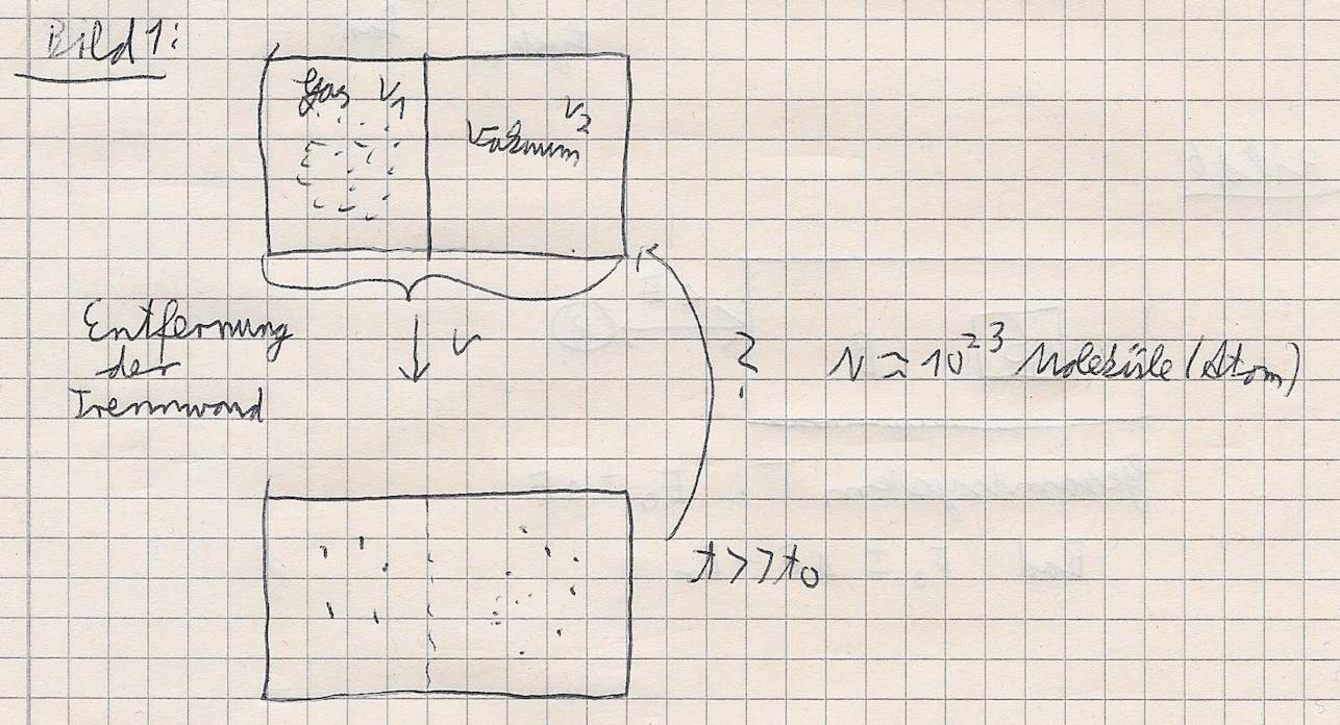
\includegraphics[width = \textwidth]{Zeichnungen/Bild1.pdf}
  \caption{Irreversibilität.}
  \label{fig:Bild1}
\end{figure}

\begin{itemize}
    \item Reversibel: Ein Prozess lässt sich spurlos umkehren.
    \item Irreversibel: Ein Prozess, der in der Umgebung eine Spur hinterlässt.
\end{itemize}
\enquote{Messfehler}: Auflösungsgrenze in Raum und Zeit.
$\Rightarrow$ Mittelungen

\begin{figure}[H]
  \centering
  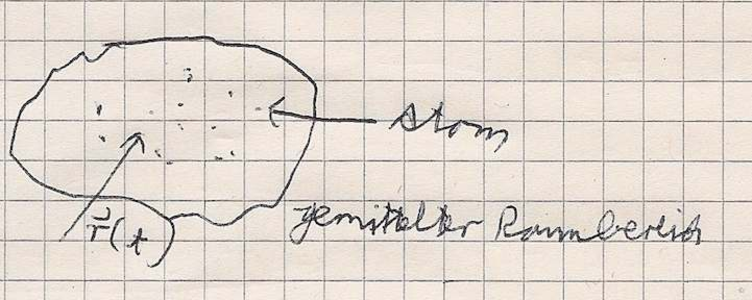
\includegraphics[width = \textwidth]{Zeichnungen/Bild2.pdf}
  \caption{Atome in Raumbereich.}
  \label{fig:Bild2}
\end{figure}
\subsection{ETH: Eigenzustand-Thermalisierungshypothese}

\begin{figure}[H]
  \centering
  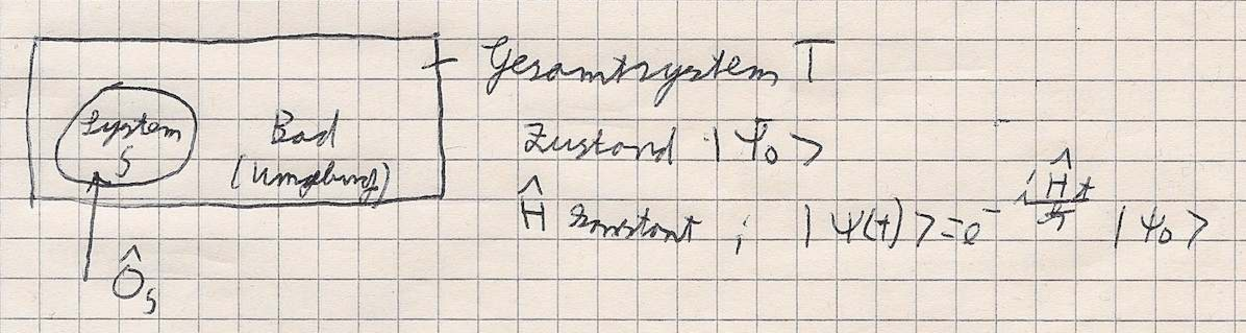
\includegraphics[width = \textwidth]{Zeichnungen/Bild3.pdf}
  \caption{Gesamtsystem und betrachtetes System.}
  \label{fig:Bild3}
\end{figure}

\begin{align}
    \Braket{O_S (t)} &= \Braket{\psi(t)|\hat{O_S} |\psi(t)}\\
    &= \Braket{\Psi_0| \symup{e}^{\frac{i H t}{\hbar}} O_S\,
    %\hat{1} = \sum_k |n><n|
    \symup{e}^{-\frac{i H t}{\hbar}}|\psi_0}\\
    &= \sum_k \Braket{\Psi_0 | \symup{e} ^ {-\frac{iHt}{\hbar}} | k} \Braket{k| \hat O_S \symup{e}^\frac{-iHt}{\hbar} | \Psi_0}\\
    &= \sum_k \langle k| \hat O_S \symup{e} ^ {-\frac{iHt}{\hbar}} \underbrace{| \Psi_0 \rangle \langle\Psi_0|}_{\hat \rho_0} \symup{e} ^ {-\frac{iHt}{\hbar}}|k\rangle\\ %\hat{rho}_0 &= |\Psi_0><\Psi_0|
    &= \sum_k \Braket{k| \hat O_S \symup{e} ^ {-\frac{iHt}{\hbar}} \rho_0 \symup{e} ^ {\frac{iHt}{\hbar}} | k}\\
    &= \Tr[\hat O_S \rho(t)]
\end{align}

\begin{align}
   \rho(t) &= \symup{e}^{-\frac{i H t}{\hbar}} \rho_0 \symup{e}^{\frac{i H t}{\hbar}}\\
    \hat \rho_0 \hat \rho_0 &= \hat \rho_0^2 = \hat \rho_0 \\
    \hat \rho_0^2 &\neq \hat \rho_0 \quad \text{Gemisch} 
\end{align}

Eigenbasis zu $\hat H$: \\
\begin{equation}
    \hat H \Ket{E_n} = E_n \Ket{E_n}
\end{equation}

\begin{align}
    \Braket{O_S(t)} &= \sum_{n,m} \Braket{E_n| O_S|E_m}
    \Braket{E_m| \symup{e}^{-\frac{i H t}{\hbar}} \rho_0 \symup{e}^{\frac{i H t}{\hbar}} |E_n}
\end{align}

\begin{align}
   \Aboxed{\Braket{O_S(t)} &= \sum_{k,m} = O^S_{n m} \rho_{m, n}^0 \symup{e}^{\frac{i}{\hbar} (E_n-E_m)t}}
\end{align}


System T: 
\begin{itemize}
    \item $N \sim10^{23} \rightarrow \infty$
    \item $E_N \rightarrow \infty$ (groß)
\end{itemize}

\begin{figure}[H]
  \centering
  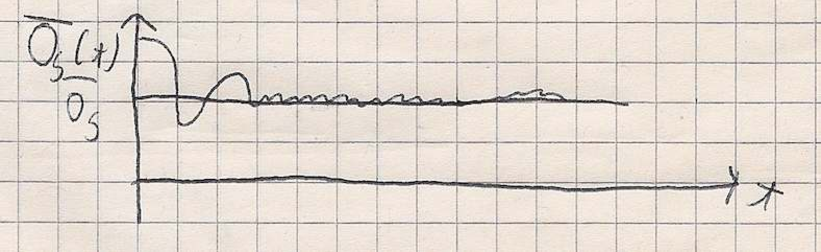
\includegraphics[width = \textwidth]{Zeichnungen/Bild4.pdf}
  \caption{Zeitlicher Verlauf von $O_S(t)$.}
  \label{fig:Bild4}
\end{figure}

\begin{align}
   \overline{O_S} &= \lim_{T \rightarrow \infty} \frac{1}{T} \int^T_0 \, \symup{d}t \Braket{O_S(t)} \\
    &= \sum_{n, m} O^2_{n, m} \rho^0_{mn} \underbrace{\lim\limits_{T \to \infty}\frac{1}{T} \int_0^T \symup{d}t
    \symup{e}^\frac{i(E_n - E_m) t}{\hbar}}_{\delta_{E_n, E_m}} \\
    \overline{O_S} &= \sum_{n,m} O^S_{n,m} \underbrace{\rho^0_{m,n} \delta_{E_n, E_m}}_{\bar\rho_{m,n}}\\
    &= ... = \Tr [\hat{O_S} \underbrace{\hat{\bar\rho}]}_\text{effektiver Dichteoperator}
\end{align}





$\Rightarrow$ Scharmittel\\
Zeitmittel $\hat{=}$ Scharmittel


\begin{align}
    \overline{\rho_{n,m}} &\equiv \rho^0_{n,m} \delta_{E_n, E_m} \Rightarrow [\hat{\bar\rho}, H] = 0 \\
    \bar{\rho}^2 &\neq \bar{\rho}\\
    [\bar\rho \vec\rho]_{n,m} &= \sum_k \bar \rho_{n, k} \bar \rho_{k,m} \\
    &= \sum_k \rho^0_{n,k} \rho^0_{k,m} \underbrace{\delta_{E_n, E_k} \delta_{E_k, E_m}}_{=\delta_{E_k, E_m}} \neq \bar \rho_{n, k}
\end{align}

$\Rightarrow$ Es entsteht ein Gemisch.

%Kasten drum
\begin{align}
    \bar{\rho} &= \sum_r \bar{\rho}\Ket r \Bra r%bis hier
    , \sum_r \bar{\rho_r} = 1
\end{align}

ETH: $\bar\rho$ Thermodynamischer Dichteoperator

\begin{figure}[H]
  \centering
  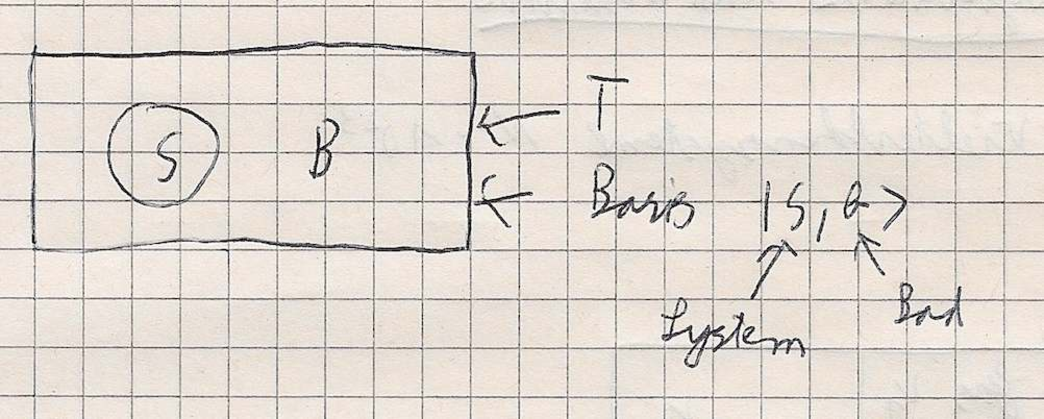
\includegraphics[width = \textwidth]{Zeichnungen/Bild5.pdf}
  \caption{System und Basis.}
  \label{fig:Bild5}
\end{figure}

\begin{align}
    \Ket{\Psi_0} &= \sum_{s,b} c_{s,b} \Ket{s,b} ,& \Braket{s,b|\hat O_S | s', b'} &= \delta_{b,b'} \Braket{s|\hat O_S|s'}\\
    \Braket{\Psi_0| \hat O_S |\Psi_0} &= \sum_{s, b}\sum{s', b'} c^{*}_{s,b} c_{s',b'} \Braket{s, b|\hat O_S| s', b'} \\
    &= \sum{s,s'} \Braket{s|\hat O_S|s'} \underbrace{\sum_b c_{s'b} c^{*}_{bs}}_{\rho^\text{red}_{s's}} \\
    &= \sum{s, s'} O^S_{s, s'} \rho^{\text{red}}_{s', s} \\
    [\rho^\text{red}]^2 &\neq [\rho^\text{red}]
\end{align}

\subsection{Gleichgewicht und Quantenstatistik}

\begin{align}
    \rho_{E_n} &= \rho_{E_m}, \quad \text{falls } E_n = E_m\\
    &= \rho(E)
\end{align}

\begin{figure}[H]
  \centering
  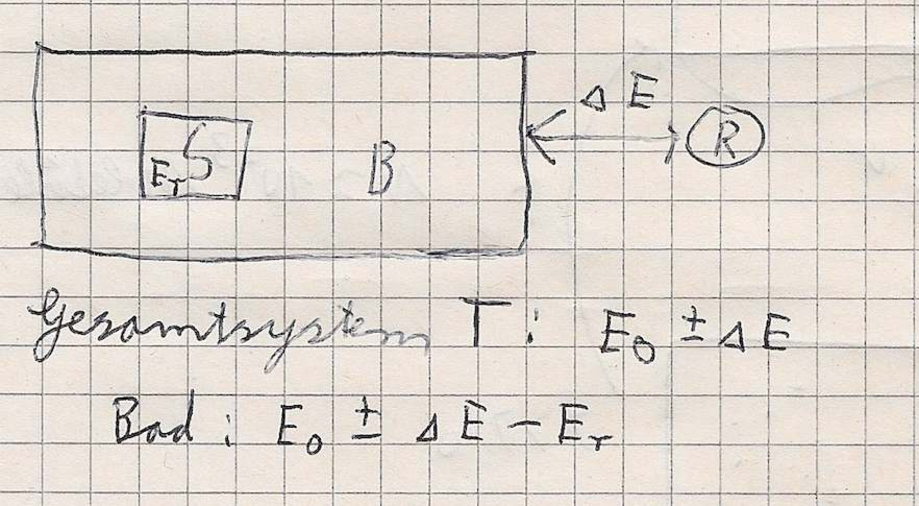
\includegraphics[width = \textwidth]{Zeichnungen/Bild6.pdf}
  \caption{System und Restsystem.}
  \label{fig:Bild6}
\end{figure}

\begin{align}
    \text{Gesamtsystem T: } E_0 &\pm \Delta E\\
    \text{Bad: } E_0 &\pm \Delta E - E_r = H_r\\
    \text{\#Zustände mit } H_r = E_0 &\pm \Delta E - E_r \eta (H_r) 2 \Delta E
\end{align}

\begin{align}
    \frac{\rho^S(E_r)}{\rho^S(E_{r'})} = \frac{\eta(H_r)}{\eta(H_{r'})} = \symup{e} \\
    E_0 \gg E_r, E_{r'} \\
    \frac{\symup{d}}{\symup{d}E} \ln \eta(E) = \beta(E_0) \stackrel{~}{~} \text{const.} \\
    \rho^S(E_r) = 1/Z \symup{e}^{-\beta E_r}, Z  = \sum_r \symup{e}^{-\beta E_r}
\end{align}

\subsection*{Wiederholung}
Zeitmittel $\hat{=}$Scharmittel
\begin{align}
    \overline{O_S} &= \lim\limits_{T \to \infty} \frac{1}{T} \int_0^T \symup{d}t \, \Braket{\underbrace{\hat O_S(t)}_{\Tr[\hat \rho_0 \hat O_S(t)]}} \\
    &= \Tr[\overline{\rho} \hat O_S(t)]\\
    &= \Tr[\hat O_S \overline \rho]
\end{align}

\begin{align}
    [\hat{\overline\rho}, \hat H = 0], \text{aber}\, [\hat O_S, \overline{\rho} \neq 0]
\end{align}


\begin{align}
    \hat \rho_0 &= \Ket{\Psi_0} \Bra{\Psi_0}
\end{align}

\begin{align}
    \overline{\rho} \neq \Ket{r}\Bra{r},\ \text{da}\ \overline{\rho}_{s,s'} \rightarrow  \text{Diagonalisierung} \rightarrow \rho_r : \overline{\rho} = \underbrace{\sum_{r} \rho_r \Ket{r}\Bra{r}}_{\text{Spektralzerlegung}} 
\end{align}

%Bild7

\begin{align}
    \Longrightarrow \Aboxed{\sum_{r}\rho_r=1}
\end{align}

%Bild8

\begin{align}
    \text{Gesamtsystem hat die Energie} &E_0\pm \increment E\\
    \text{System S:}\ &E_r\\
    \Rightarrow \text{Bad B:}\ &H_r=E_0-E_r\pm \increment E
\end{align}

Wahrscheinlichkeit für die Energie $E_r$: $\rho_s(E_r)$\\
\# Anzahl der Kombinationen (Zustände) mit Energie $H_r$ im Bad:

\begin{align}
    = \eta(E_0-E_r) 2 \increment E \\
    \increment E \to 0 \, \text{für} \, N \to \infty  
\end{align}



\begin{align}
    \frac{\rho_s(E_r)}{\rho_s(E_{r'}} 
    &= \frac{\eta(E_0-E_r)\cancel{2 \increment E}}{\eta(E_0-E_{r'})\cancel{2\increment E}} \\
    &= \symup{e}^{\ln \eta (E_0 - E_r) - \ln \eta (E_0 - E_{r'})}\\
    &\approx \symup{e}^{\beta (E) (-E_r + E_{r'})}\\
    &= \symup{e}^{-\beta  (E_r - E_{r'})}\\
    E_0 &\gg E_r, E_{r'} \\
\intertext{Nebenrechnung, Taylorreihe: }
    \ln \eta(E_0-E_r) &= \ln \eta(E_0) + 
    \underbrace{\frac{\symup{d}}{\symup{d}E} \ln\eta(E) \bigg|_{E_0}}_{\beta(E)} 
    (E_0 - E_r) + O((E_0 - E_r)^2) \\
    [\beta(E)] &= [\frac{1}{E}]
\end{align}

% Weiß jemand was das hier ist ?????????? nebenrechnung
\begin{align}
    \sum_{r} \rho(E_r) = 1 \\
    \rho(E_r) \propto \symup{e}^{-\beta(E) E_r}
\end{align}

\begin{align}
    \intertext{Zustandssumme Z}
    Z=\sum_{r}^{} e^{-\beta E r} = e^{-\beta F}\\
    \intertext{Parametrisierung der Zustandssummen mit F : Helmholtzsche \enquote{Freie Energie}}
    \Rightarrow \rho(E_r) = \frac{1}{Z} \symup{e}^{-\beta E_r}
\intertext{Mit der Annahme $\beta(E) \approx$ konst.}
    \beta &=\frac{1}{k_\text{B}T} \\
\end{align}

\begin{align}
    T:& \text{Temperatur}\\
    k_\text{B}:&\text{Boltzmankonstante} 
\end{align}

Freie Energie
\begin{align}
F = - \frac{1}{\beta} \ln (Z) = F(T,V)\\
T : \text{intensive Größe}\\
V: \text{extensive Größe} \Rightarrow V \propto N\\
F: \text{extensive Größe}
\end{align}
Additivität von Teilsysteme $A+B$   

\begin{align*}
%    \Aboxed{{\Aboxed A} {\Aboxed B}} % geht nichzt :(
\end{align*}

\begin{align}
    \rho{A+B} &= \frac{1}{Z_{A+B}}\symup{e}^{-\beta E}\\
    &= \rho_A(E_A)\ \rho_B(E_B) \\
    &= \frac{1}{Z_A Z_B} \symup{e}^{-\beta(E_A + E_B)}\\
\text{mit:}\, E = E_A + E_B
    \rightarrow Z_{A+B}&=Z_A Z_B\\
    \rightarrow F_{A+B}&=-\frac{1}{\beta}\ln(Z_{A+B})=F_A F_B :\text{F ist additiv}
\end{align}

\subsection{Einführung der Entropie}
Innere Energie $U$ 


\begin{align}
    U=\Braket{\hat H_S}% &= \Tr[\overline{\rho}\hat H_S]\\
    &=\sum_{r}\frac{\symup{e}^{-\beta E_r}}{Z} E_r \\
    &= -\frac{\partial}{\partial \beta} \ln Z\\
    U-F &=\frac{1}{Z} \sum_{r} e^{-\beta E_r} E_r \frac{\beta}{\beta} + \frac{1}{\beta} \ln Z 
    \left(\frac{1}{Z} \sum_{r} e^{-\beta E_r} \right) \\
    &= \frac{-1}{Z\beta} \sum_r e^{-\beta E_r} \underbrace{-\beta E_r -\ln Z}_{\underbrace{\ln(e^{-\beta E_r - \ln Z})}_{\rho(E_r)}}\\
    &=T(-k_\text{B}) \sum_{r} \rho(E_r) \ln \rho(E_r) = \text{TS}
\end{align}


mit der Entropie S
\begin{align*}
    S &= -k_\text{B} \sum_r \rho (E_r ) \ln \rho(E_r) \leq  0 \\
    1\leq \rho &\leq 0 \\
    \ln(x) &\geq 0 \ \text{Für}\ x\geq 1  \\
    \Aboxed{U&\leq F} \\
    \Rightarrow F(T,U) = U-TS \,\,\,\,&\hat{=}\,\,\,\, U =F+TS
\end{align*}

\subsection*{Wiederholung?}
\begin{align}
\intertext{Freie Energie}
    F(T, V) &= - \frac{1}{\beta} \ln Z, \frac{1}{\beta} = k_\text{B} T \\
\intertext{Zustandssumme}
    Z &= \Tr[\symup{e}^{-\beta \hat H}] = \sum_n \symup{e}^{-\beta E_n} = \symup{e}^{-\beta F} \\
\intertext{Innere Energie}
    U &= \Braket{\hat{H}}=\frac{1}{z} \sum_{n}e^{-\beta E_n} E_n \\
    U-F&=TS=T\left(-k_\text{B}\sum_{n} \underbrace{\frac{1}{z}e^{-\beta E_n}}_{\rho_n} \ln(\rho_n)\right)
\intertext{Entropie}
    S &= -k_\text{B} \sum_n \rho_n \ln \rho_n = - k_\text{B} \Braket{\ln\rho_n}\\
    S[\hat\rho] &= -k_\text{B} \Tr[\hat\rho \ln\hat\rho]
\intertext{Totales Differential}
    \symup{d} F &= \left(\frac{\partial F}{\partial V}\right)_T \symup{d} V +
    \left(\frac{\partial F}{\partial T}\right)_V \symup{d} T\\
    - \left(\frac{\partial F}{\partial T}\right)_V  &= \partial_T (U_B T \ln Z) = \frac{k_\text{B} T}{T} \ln Z + k_\text{B} T \frac{1}{Z} \frac{\partial}{\partial T} Z\\
    \frac{\partial}{\partial T} &= \frac{\partial \beta}{\partial T} = -k_\text{B} \beta^2 \frac{\partial}{\partial \beta}\\
    &= - \frac{1}{T} F + \frac{1}{T} \underbrace{\frac{1}{Z} \sum_n (+E_n) \symup{e}^{-\beta E_n}}_{U}\\
    -\left(\frac{\partial F}{\partial T}\right)_V&=\frac{1}{T}(U-F)=S \\
    (\frac{\partial F}{\partial V})_T &= -P\\
    \left[-\frac{\partial H}{\partial x}\right] &\propto [\text{Kraft}]\\
    \left[-\frac{\partial H}{\partial V} \right]&=\left[ \frac{\mathrm{Kraft}}{\mathrm{Fläche}}\right]=P\ (\mathrm{Druck}) 
\end{align}

\underline{Genauer:}
\begin{align}
    - \pdif{F}{V}[T] &= \frac{1}{\beta} \pdif{}{V} \ln Z=  \frac{1}{\cancel{\beta}} \frac{1}{Z} \sum_n \left(-\cancel{\beta} \frac{\partial}{\partial V} E_n\right) \symup{e}^{-\beta E_n} = -\frac{1}{Z} \sum_n \symup{e}^{-\beta E_n} \pdif{E_n}{V}[]\\
    &= - \Braket{\frac{\partial H}{\partial V}} \geq 0 \\
\intertext{Beispiel: Potentialtopf:}
    E_n &= \frac{\pi^2 \hbar^2}{2m} \frac{n^2}{L^2} \propto \frac{1}{V^{\sfrac{2}{a}}} \\
    \pdif{E_n}{V} &\propto - \frac{2}{a} \frac{1}{V} \frac{1}{V^{\sfrac{2}{a}}} 
\end{align}
\begin{align}
    \symup{d} F &= -p\symup{d} V- S \symup{d}T\\
    F &= U-TS\\
    U &= F +TS\\
    \symup{d}U &= \symup{d}F + \symup{d}(TS) = (-p \symup{d}V - S \symup{d} T) + T \symup{d}S + S \symup{T}\\
    &= -p \symup{d}V + T \symup{d}S\\
    \Rightarrow U &= U(V,S)  \quad \text{U ist Legendre-Transformatierte von}\ F(V,T)
\end{align}
\begin{align}
    \Aboxed{\left(\frac{\partial U}{\partial S} \right)_V = T} \geq 0 \quad \text{d.h. Definition der Temperatur}
\end{align}

\subsection{Interpretation des Entropie-Begriffs}

\begin{align}
    S &= - k_\text{B} \sum_n \rho_n \ln \rho_n = -k_\text{B} \Tr[\hat \rho \ln\hat\rho]
\end{align}
Beispiel: Spin-System mit M Spin 1/2 : Hilbertraum -Dim.: $D=2^M$
\begin{align}
    M = 4 \Rightarrow D = 2^4 = 16
\end{align}
Anzahl der Fragen zum Zustandsrest:

%Bild 9

Informationsinhalt: $ M = \log_2 D$
\begin{align}
    \# \text{Fragen} &\propto \ln D\\
    \text{Gleichverteilung:  }\rho_n &= \frac{1}{D}\\
    S &= -k_\text{B} \underbrace{\sum_n \rho_n}_{=1} \cdot \ln \frac{1}{\beta} = k_\text{B} \ln D\\
\end{align}
Entropie: Maß für unser Unwissen über das System
Wir maximieren die Entropie
\begin{align}
    S[\hat \rho] &= -k_\text{B} \Tr [\hat \rho \ln \rho]\quad \text{Funktional}\\ 
\intertext{Nebenbedingung}
    \Tr[\hat \rho] &= 1 = \sum_n \rho_n \\
    I[{\rho_n}] &= S [{\rho_n}] + k_\text{B} \lambda_0 \left(\sum_n \rho_n -1\right)\\
    \delta I &= 0\\
    \Rightarrow \frac{I}{\rho_n} &= - k_\text{B} \frac{\partial}{\partial \rho_n} \left[\sum_n \rho_{n'} \ln \rho_{n'} - \lambda_0\left(\sum_n \rho_n -1\right)\right]\\
    &=  -k_\text{B} [ \underbrace{\ln \rho_n +1}_{= 0} - \lambda_0] = 0 \\
    \Rightarrow \rho_n &= \symup{e}^{\lambda_0 -1} \quad \text{Gleichverteilung}
\end{align}
\begin{align}
    \sum_n \rho_n = 1 = \sum^D_{n=1} \symup{e}^{\lambda_-1} &= \symup{e}^{\lambda_-1}D \Rightarrow \symup{e}^{\lambda_-1} = \frac{1}{D} = \rho_n\\
    \intertext{Maximum ?}
    \eta(x) &= -x \ln x \\
    \eta' (x) &= -(\ln x +1)\\
    \eta''(x) &= - \frac{1}{x} \quad < 0 \quad x > 0\quad \text{Maximum}
\end{align}

\subsection{von-Neumann-Gleichung}

\begin{align}
    i \hbar \partial_t \Ket{\Psi} &= \hat H \Ket{\Psi}\\
    \hat \rho (t) &= \sum_n p_n \Ket{n(t)} \Bra{n(t)}\\
    i \hbar \Ket{n(t)} &= \hat H \Ket{n(t)}\\
    - i \hbar \Bra{n(t)} &= \Bra{n(t)} H\\
    \frac{\partial}{\partial t}\hat\rho(t) &= \sum_n P_n \left[\left( \frac{\partial}{\partial t} \Ket{n(t)}\right) \Bra{n(t)} + \Ket{n(t)} \left( \frac{\partial}{\partial t} \Bra{n(t)} \right) \right]\\
    &= \frac{1}{i \hbar} \sum_n p_n \left[\hat H \Ket{n(t)} \Bra{n(t)} - \Ket{n(t)} \Bra{n(t)} \hat H\right] \\
    \Aboxed{
        \frac{\partial \rho (t)}{\partial t} &= \frac{i}{\hbar} \left[\hat \rho(t), \hat H \right]
    }  \quad \text{von-Neumann-Gleichung}
\end{align}


\subsection{Wahrscheinlichkeitsverteilung und zentraler Grenzwertsatz}

Würfel: Mit welcher Wahrscheinlichkeit würfel' ich die Zahl $X$ \\
Antwort: $P$


\begin{align}
    N &\ \text{Ereignisse} \\
    Q: w_N(n) &= p^n (\underbrace{1-p}_{q})^{N-n}
\intertext{$n$ mal die Zahl $X$ zu finden:}
    \sum_{n=0}^{N} w(n) &= \sum_{n=0}^N \binom{N}{n} p^n q^{N-n} = (\underbrace{p+q}_{=1})^N = 1\\
    N\to\infty
\end{align}
\subsubsection*{Statistische Verteilungsfunktion für eine kontinuierliche Variable $X: w(x)$}
Statistische Mittelung von $f(x)$
\begin{align}
    \Braket{f} &= \int_{-\infty}^\infty \symup{d}x w(x)f(x) \quad \left[ \Braket{f} = \frac{1}{N} \sum^N_{i=1} f(x_i) \right]\\
    p(x) &= w(x)\symup{d} x, \quad x\in[x,x+\symup{d}x] \\
    \intertext{Normierung}
    \Braket{1}&= \int_{-\infty}^\infty \symup{d}x w(x)=1
\end{align}
\paragraph{Charakteristische Funktion:}
\begin{align}
    \tilde w(k) &= \Braket{\symup{e}^{-ikx}} = \int_{-\infty}^\infty \symup{d} x w(x) \symup{e}^{-ikx} \quad \text{FT von}\ w(x) \\
    \Rightarrow w(x)&=\int_{-\infty}^\infty \frac{\symup{d}k}{2\pi}\ \tilde w(x) e^{ikx} \\
    \Rightarrow \tilde w(0)&=1 \quad \text{(Normierung)}
\end{align}

\paragraph{Taylor-Reihe}
\begin{align}
    \tilde w(k) &= \Braket{\sum^\infty_{n=0} \frac{(-ik)^n}{n!} x^n}
    =\sum_{n=0}^{\infty} \frac{(-ik)^{n}}{n!} \underbrace{\Braket{x^n}}_{\text{Momente der Verteilung}}
\end{align}
Charakteristische Funktion enthält \emph{alle} Momente der Verteilung 
\begin{align}
    \Rightarrow \Braket{x^n} &= i^n \frac{\symup{d}^n}{\symup{d}k^n}\tilde w(k) \Bigg|_{k=0}
\end{align}
\paragraph{Kumulanten:}
Maß für Fluktuationen
\begin{align}
    \ln \tilde w(k)&=\ln \Braket{\symup{e}^{-i kx}} = \sum_{n=1}^\infty \frac{(-i k)^n}{n!} \Braket{x^n}_C\\
    \stackrel{\text{Taylorreihe}}{\Rightarrow} \Braket{x^n}_C &= i^n \frac{\symup{d}^n}{\symup{d}k^n}[\ln(\tilde w(k)] \bigg|_{k=0}\\
\end{align}
\begin{align}
    n=1&: \quad \Braket{x}_C = i\frac{\symup{d}}{\symup{d}k}[\ln \tilde w(k)]=i\frac{\tilde w'(k)}{\tilde w(k)}\bigg|_{k=0} = i \tilde w'(0) = \Braket{x} \\
    n=2&: \quad \Braket{x^2}_C = i^2 \frac{\symup{d}}{\symup{d}k} \left[\frac{\tilde w'(k)}{\tilde w(k)}\right]_{k=0} \\
    &\quad= i^2 \left[\frac{\tilde w''(k)}{\tilde w(k)}-\frac{\tilde w'(k)^2}{\tilde w(k)^2}\right]_{k=0}\\
    &\quad = [i^2 \tilde w''(k) - (i w')^2]_{k=0}\\
    \Aboxed{\Braket{x^2}_C &= \Braket{x^2}  \Braket{x}^2 = \sigma ^2} \quad \text{Kumulante 2. Ordnung}
\end{align}
\begin{align}
\intertext{Annahme:}
    \ln \tilde w (k) &\approx -i k\Braket{x} + \frac{(ik)^2}{2}\Braket{x^2}_C+O(\Braket{x^3}) \\
    \Rightarrow \tilde w(n) &= \symup{e}^{ik \Braket{x}+ \frac{(-ik)^2}{2}\Braket{x^2}_C}
\intertext{F.T.}
    w(x) &= \int_{-\infty}^\infty \frac{\symup{d}k}{2\pi} \symup{e}^{ikx} \symup{e}^{-ik \Braket{x} - \frac{k^2}{2} \Braket{x^2}_C}\\
    &= \int_{-\infty}^\infty \frac{\symup{d}k}{2\pi} \exp\left({-\frac{\Braket{x^2}_C}{2} \left[\underbrace{k^2-2i k \frac{x-\Braket{x}}{\Braket{x^2}_C} + \frac{[i (x -\Braket{x})]^2}{\Braket{x^2}_C^2}}_{\overline k ^2} - \frac{[i (x -\Braket{x})]^2}{\Braket{x^2}_C^2}\right]}\right)\\
    &= \exp\left({-\frac{1}{2}\frac{(x-\Braket{x})^2}{\Braket{x^2}_C}} \cdot \frac{1}{\sqrt{2 \pi \Braket{x^2}_C}}\right)\\
    \Rightarrow \text{Gaußverteilung}
\end{align}

%Bild 10

Charakteristische Funktion als diskrete Fourier-Transformation von $w_N(n)$
\begin{align}
    \tilde w _N (k) &= \Braket{\symup{e}^{-i kx}} = \sum_{n=0}^N w_N(k) \symup{e}^{-ikn}\\
    &= \sum_{n=0}^N \binom{N}{n} \underbrace{p^n q^{N-n}}_{(p\symup{e}^{-ik})^n} \symup{e}^{-ikn} = (p \symup{e}^{-ikn} +1)^N\\
    \Rightarrow \ln \tilde w(n) &= N \ln(p \symup{e}^{-ikn} +q)\\
\intertext{ $\Rightarrow$ alle Kummulanten $\propto N$ }
    \Braket{k} &= i\frac{d}{d k} \ln \tilde w'^(k)_N \bigg|_{k=0} = iN \frac{-ip \symup{e}^{-ik}}{p \symup{e}^{-ik}+q} \bigg|_{k=0} = N \cdot P\\
    \Braket{k^2}_C &= i \frac{\symup{d}}{\symup{d}k} \left[i N \frac{-i p \symup{e}^{-ik}}{p\symup{e}^{-ik +q}}\right] = ... = N p q = \sigma^2
\intertext{relative Abweichung}
\frac{\sigma}{\Braket{n}}&=\frac{\sqrt{\Braket{n^2}_c}}{\Braket{n}} =\frac{\sqrt{N p q}}{Np}=\frac{1}{\sqrt{N}}\sqrt{\frac{q}{p}}\propto \frac{1}{\sqrt{N}}\\
\intertext{Zentraler Grenzwertsatz:}
\intertext{intensive Größen:}
    x &= \frac{n}{N} \quad 0 \leq x \leq 1\\
    \bar x &= \frac{\Braket{n}}{N}=p ; \: \: \bar \sigma^2 = \frac{\sigma^2}{N}= pq\\
    w_N (n=N x) &= \frac{1}{\sqrt{2 \pi N \bar \sigma^2}} \symup{e}^{-\frac{1}{2}\frac{(x-\Braket{x^2})^2}{2 \frac{\overline \sigma^2}{N}}}\\
    w_N(n) \underbrace{\symup{d}n}_{N \symup d x} &= w_N(x) \symup{d}x \\
    \sigma_\text{eff.} &= \frac{\bar \sigma^2}{N} \rightarrow 0\\
    w_N(x) &= \frac{1}{\sqrt{2 \pi \frac{\overline{\sigma}^2}{N}}} \exp \left({-\frac{(x-\Braket{x})^2}{2 \overline \sigma^2/N}}\right)
\end{align}
\paragraph{Gesetz der großen Zahlen}
\begin{align}
    X&: X_1, X_2, ..., X_N \quad \text{Sequenz von Zufallszahlen}\\
    \mu &= E(X), \: \: \sigma^2 = \text{Var}(X)\\
    \intertext{Realisierung:}
    M &= \frac{1}{n} \sum^n_{k=1} X_n\\
    E[M]&=\mu \\
    \Var(M) &= \frac{\sigma^2}{n} \xrightarrow{n\to\infty} 0
\end{align}
\paragraph{Zentraler Grenzwertsatz}
\ \\
$X_1, X_2,...., X_n$ Reelle Zufallsvarianz der Gleichverteilung $w(X)$
\begin{align}
    Y_n &= \sum_{i=1}^{n} X_i\\
    \intertext{Mittelung}
    M_n &= \frac{Y}{n} \xrightarrow{n\to\infty} M \Rightarrow \Braket{Y_n} = nM = E[Y_n]\\
        &\Braket{Y_n^2}-\Braket{Y_n}^2=n\sigma^2\\
    \intertext{Normierung}
    Z_n &= \frac{Y_n-n\mu}{\sqrt{n}\sigma} \Rightarrow \Var(Z_n) = 1 \rightarrow w(Z) = \frac{1}{\sqrt{2\pi}} \symup{e}^{-\frac{1}{2}Z^2}
\end{align}
\section{Axiome der Thermodynamik}

\subsection*{Axiom 1: Gleichgewichtszustand}
Es existiert ein spezieller Zustand eines einfachen Systems, der Gleichgewichtszustand genannt wird, welcher makroskopisch durch die innere Energie U , das Volumen V und die Gesamtzahlen $N_1, N_2, ..N_k$ der $k$ verschiedenen chemischen Komponenten des Systems
vollständig bestimmt ist.

\subsection*{Axiom 2: Postulate der Entropie-Maximierung}
Es existiert eine Funktion, die Entropie genannt wird und eine Funktion der extensiven Parameter des Systems ist, die für alle thermodynamischen Zustände definiert ist und folgende Eigenschaft hat: Die Werte, die die extensiven Parameter annehmen in Abwesenheit von internen Zwangsbedingungen sind diejenigen, die die Entropie über die Menge der erlaubten thermodynamischen Zustände maximieren.

\subsection*{Axiom 3: Additivität der Entropie}
Die Entropie eines zusammengesetzten Systems setzt sich additiv aus den Entropien der Teilsysteme zusammen. Die Entropie ist stetig differenzierter und eine monoton wachsende Funktion der Energie.

\subsection*{Axiom 4: Dritter Hauptsatzes der Thermodynamik}
Die Entropie eines jeden Systems verschwindet in dem Zustand für den
\begin{align}
    \left( \frac{\partial U}{\partial S}\right)_{V, N_i} = 0 
\end{align}
gilt, was bei $T = 0$ der Fall ist.

\subsection{Der zweite Hauptsatz der Thermodynamik}

\paragraph{Erster Hauptsatz: Energieerhaltung}
\begin{align}
    \underbrace{\increment U}_{\text{Innere Energie}} &= \underbrace{\increment Q}_{\text{Wärme}}-\underbrace{\increment W}_{\text{Arbeit}}
\end{align}
\paragraph{Zweiter Hauptsatz}
Jeder Prozess, der ein thermisch isoliertes System von einen Makrozustand A nach B überführt lässt die Entropie konstant oder führt zu einem Anstieg von $S$.
\begin{align}
    \Aboxed{\symup d S \geq 0}
\end{align}

\begin{align}
\intertext{Reversibler Prozess:}
    \increment S_\text{Gesamt} &= 0 = \increment S_\text{System} + \increment S _\text{Umgebung} \\
\intertext{Irreversibler Prozess:}
    \increment S_\text{Gesamt} &> 0
\intertext{Entropiefunktional:}
    S[\hat \rho] &= -k_\text{B} \Tr[\hat \rho \ln(\hat \rho)]\\
    \frac{\symup{d}}{\symup{d}t}\hat \rho(t) &= \frac{i}{\hbar} [\hat \rho, H] \quad \text{von-Neumann-Gleichung}\\
    \rho(t)&= \symup{e}^{-\frac{i}{\hbar}Ht}\ \rho_0\ \symup{e}^{\frac{i}{\hbar}Ht} = U^\dagger(t) \rho_0 \hat U(t) \\
    S(t) &= S[\hat \rho(t)] = -k_\text{B} Tr[\hat U^\dagger(t) \rho_0 \hat U(t) \underbrace{\ln(\hat U^\dagger(t) \rho_0 \hat U(t))}_{\sum_{n=0}^\infty \frac{a_n}{n!}X_n}] \\
    &= -k_\text{B} Tr[\rho_0\ln\rho_0] = S[\rho_0]= \text{const.}
\end{align}

\subsection{Behandlung von teiloffenen Systemen}

\paragraph{Die kanonische Gesamtheit}
Definition: $N =$ const. , Energieaustausch
\begin{align}&
    E=\Braket{\hat H} = \text{const. , durch das Bad aufgeprägt}\\
    \Aboxed{S \leftrightarrow Bad}
\end{align}
\paragraph{Q: Was ist $\hat \rho$?}
\begin{align}
     I [ \rho] &= S[\rho] - \underbrace{\gamma (\Braket{H}-E)}_{\text{Energieinhalt}} -\underbrace{\lambda (\Braket{\hat 1}-1)}_{\text{Norm}}\\
    [\gamma]&=[\frac{k_\text{B}}{E}]   \: \: , [\lambda]=[k_\text{B}]\\
    \delta I &= 0
\end{align}
\newpage
\subsection*{Beschreibung}
\begin{table}[H]
    \centering
    \begin{tabular}{c|c}
        mikroskopisch & makroskopisch \\
        \toprule \\
        $i \hbar \partial_t \Ket{\Psi(t)} = \hat H \Ket{\Psi}$& Freie Energie \\
        $\dot q_i = \frac{\partial H}{\partial p_i}$ & $F(V,T)=U-T\underbrace{S}_{\text{Entropie}}$\\
        $\dot p_i = \frac{\partial H}{\partial q_i}$ & $S=-\left(\frac{\partial F}{\partial T}\right)_V$ \\
        \ & $p = - \left(\frac{\partial F}{\partial V}\right)_T$\\
        \ & $U = F+ TS = U(V, S)$\\
        \ & Thermodynamik \\
    \end{tabular}
    \caption{Beschreibung}
    \label{tab:1}
\end{table}
$\longleftrightarrow$
Statistik: $\hat \rho , \rho( {q_i, p_i})$

\paragraph{Kanonische Gesamtheit}

\begin{align}
\intertext{$E = \Braket{H} \quad$ Konstant, durch ein Bad reguliert}
    \I[\hat{\rho}] &= S[\hat{\rho}] - \lambda(\underbrace{\Braket{\hat{\mathbb 1}}}_{\Tr[\hat\rho]}-1)
    +\gamma\left(\Braket{\hat H}-E\right)\\ 
\intertext{Maximum der Entropie}
    \I[\hat \rho + \delta \rho ]-\I[\rho] &= -k_\text{B} \Tr[\delta \rho \underbrace{(\ln(\rho) + 1 + \frac{\lambda}{k_\text{B}}+ \frac{\gamma}{k_\text{B}}\hat{H}}_{=0}] = 0 \\
\intertext{$\delta \rho$ beliebig}\\
    \Rightarrow \ln(\hat \rho) + &1+ \lambda_0 + \frac{\gamma}{k_\text{B}}\hat H = 0\\
    \Aboxed{\hat \rho &= \symup{e}^{-(1 + \lambda_0)} \symup{e}^{-\frac{\gamma }{k_\text{B}}\hat H}}
\end{align}

\begin{align}
    \intertext{Def: $\beta=\frac{1}{k_\text{B}T}=\frac{\gamma}{k_\text{B}}$}
    \Tr[\rho]&=1 \Rightarrow \symup{e}^{-(1+\lambda_0)}=\frac{1}{\Tr[\symup{e}^-\beta \hat H]}\\ 
    \hat{\rho} & = \frac{1}{Z_\text{kan}} \symup{e}^{-\beta\hat{H}}, \quad \text{$Z_\text{kan}$ Kanonische Zustandssumme}\\
    Z_\text{kan} &= \Tr[\symup{e}^{-\beta \hat H}] \\
    E &= \Braket{H} = \frac{1}{Z_\text{Kan.}} \Tr[\symup{e}^{-\beta \hat H} \hat H] = -\frac{\partial}{\partial \beta}\ln(Z_\text{kan}(\beta))
\intertext{Entropie}
    S_\text{kan}&=S[\hat\rho_\text{kan}]=-k_\text{B} \Tr\left[\underbrace{\frac{1}{Z_\text{kan}} \symup{e}^{-\beta \hat H}}_{\rho}\ln\left(\frac{1}{Z_\text{kan}}e^{-\beta H}\right)\right] \\
    &=k_\text{B} \ln(Z_\text{kan})+\underbrace{k_\text{B}\beta}_{\sfrac{1}{T}}\Braket{H} \\
    U &= \Tr [\rho H]\Braket{H} = T S_\text{kan}  \underbrace{-\underbrace{k_\text{B} T}_{\sfrac{1}{\beta}}\ln(Z_\text{kan})}_{+ F} = T S_\text{kan}+F=\Tr[\rho H]\\ 
    &= T S_\text{kan} + \left( - \frac{1}{\beta} \ln(Z_\text{kan}\right)\\
    \Aboxed{&\frac{\partial U}{\partial S_\text{kan}}=T}
\end{align}

\begin{enumerate}
    \item \begin{align}
        F[\hat\rho]&=U[\hat\rho]-TS[\rho]\\
        \delta F&=...=-T\delta I[\hat\rho]: \text{ Maximierung der Entropie $\hat=$ Minimierung von $F$}
        \end{align}
    \item \begin{align}
        F(T=0) &= \lim_{\beta \rightarrow \infty} F(\beta)\\
        T &=0 \quad \text{ist für endliches $\beta$  nicht erreichbar}\\
        \end{align}
    \item Gleichgewicht
        % Bild 11
        \begin{align}
            S&=S_1+S_2 \quad \text{const.}\\
            U&=U_1+U_2 \quad \text{const.}\\
            \dif U&= 0 = \dif U_1+\dif U_2 \quad \text{Energieerhaltung}\\
            \dif S&= 0 = \left(\frac{\partial S_1}{\partial U}\right)\symup{d}U_1 + \left(\frac{\partial S_2}{\partial U}\right)\symup{d}U_2\\
            &=\frac{1}{T_1} \symup{d}U_1 + \frac{1}{T_2} (-\symup{d}U_1)\\
            &= \left( \frac{1}{T_1}-\frac{1}{T_2} \right) \symup{d}U_1 = 0\\
            &\Rightarrow\text{Temperaturen müssen gleich sein} T_1=T_2
        \end{align}
\end{enumerate}

\section{Statistische Gesamtheiten oder Gleichgewichtsensembles}

QM: Observable: $\hat O_1, \hat O_2,..., \hat O_r$


\begin{itemize}
    \item $\hat O_1,...\hat O_S$: Durch ein Bad reguliert $\Rightarrow f_i = <\hat O_i>$
    \item $\hat O_{S+1},\hat O_{S+2},...,\hat O_\gamma$:  scharfe Erwartungswerte
\end{itemize}

\subsection{Generalisiertes Gibbs-Ensemble}
Funktional
\begin{align}
    \Phi [\hat \rho_S] &= -k_\text{B} \left[\Braket{\ln(\hat\rho} + \sum_{j=0}^S \lambda_j \left(\Braket{\hat O_j} -f_j\right)\right]\\
    S \text{maximal} &\Rightarrow \delta\Phi[S_i]\\
    \delta \Phi_S[\rho_j] &= -k_\text{B} \Tr\left[\delta \rho_S\left[\ln(\rho_j) +1 + \sum_{j=0}^S \lambda_j \hat O_j\right]\right] =0\\
    \Rightarrow \hat \rho_S &= \frac{1}{Z_S} \symup{e}^{-\sum_{j=1}^S \lambda_j \hat O_j}\\
    Z_S &= \exp(+(1+\lambda)) = \Tr\left[\exp\left(\sum_{j=1}^S \lambda_j \hat O_j\right)\right]\\
    \Braket{\hat O_j}&=\Tr[\hat \rho_S \hat O_j]=f_j \quad j=1,...,S\\
    Z_S&=Z(\underbrace{\lambda_1, \lambda_2,...,\lambda_S}_\text{Äußere Parameter},f_{S+1},...,f_\gamma)
\end{align}

\begin{align}
    \frac{\partial \ln(Z_S)}{\partial\lambda_0} &= \frac{1}{Z_S} \frac{\partial}{\partial \lambda_j} \Tr\left[\symup{e}^{\sum_{j=1}^S \lambda_j \hat O_j }\right] = -\Braket{O_j} = -f_j\\
    S_S &= -k_\text{B} \Tr\left[\hat \rho (-\sum_{j=1}^S \lambda_j \hat O_j -\ln(Z_S)\right]\\
        &= k_\text{B} \left(\underbrace{ln(Z_S}_{1+\lambda_0}+\sum_{j=1}^{S}\lambda_j
        \underbrace{\Braket{\hat O_j}}_{f_j}\right)\\
    \Aboxed{&\frac{\partial S_S}{\partial  f_j}=k_\text{B}\lambda_j} \\
    \text{Spezialfall: } s &= r: \quad Z_r = Z(\lambda_1,...\lambda_r)\\
    \text{Da } \lambda_1,...\lambda_r \text{intensiv } &\Rightarrow Z_r \text{intensiv}\\
    &\Rightarrow \lim_{N \to \infty} \frac{1}{N} Z_r = 0 \\
    &\Rightarrow S_r \stackrel{N \to \infty}{=} \sum_{j = 1}^r \frac{\partial S_r}{\partial  f_j} f_j
\end{align}
\begin{align}
\intertext{Duhen-Gibbs-Relation:}
    \Aboxed{\Braket{\hat H} - \mu \Braket{\hat N} + p \Braket{\hat V} - TS &= 0}
\end{align}
$\mu$: chemisches Potential. \\
Großkanonische Gesamtheit: Teilchenzahl variabel

\subsection{Geisterkapitel}
\subsection{Großkanonische Gesamtheit}
\begin{align}
    Z_\text{GK} &= \Tr [\e^{-\beta (\hat H-\mu \hat N)}] \\
    \hat O_1 &= \hat H  \longrightarrow \lambda_1=\beta\\
    \hat O_2 &= \hat N  \longrightarrow \lambda_2 = -\beta \mu \quad \mu:\text{chemisches Potential} \\
    \mu \hat N &\longrightarrow \sum_n \mu_n \hat N_n\\
\end{align}
\begin{align}
    \frac{\partial S}{\partial E} &= \frac{1}{T}=k_\text{B}\lambda_1 &
    \frac{\partial \ln(Z_\text{GK})}{\partial \beta} &= -E \\
    \frac{\partial S}{\partial N }&=k_\text{B}\lambda_2=-\frac{\mu}{T} &
    \frac{\partial \ln(Z_\text{GK})}{\partial(\beta\mu)}&=N\\
\end{align}
\begin{align}
    \frac{\partial E}{\partial \beta}&=
    \frac{\partial}{\partial\beta}\left(\frac{1}{Z_\text{GK}} \Tr[\symup{e}^{-\beta(\hat H-\mu\hat N)}\hat H]\right)\\
    &=-\frac{1}{Z_\text{GK}}\Tr[H(\hat H-\mu\hat N)\, \symup{e}^{-\beta(\hat H-\mu\hat N)} ]\\
    &\quad+ \underbrace{\frac{1}{Z_\text{GK}^2} \Tr \left[+(\hat H-\mu \hat N) \e^{-\beta(H -\mu N)}\right]\Tr[\e^{-\beta(H -\mu N)} \hat H]}_{\Braket{(\hat H - \mu N)} \Braket{\hat H}}\\
    &= -[\Braket{H^2} -\mu \underbrace{\cancel{\Braket{\hat H \hat N}}}_{\Rightarrow \Braket{\hat H}\Braket{\hat N} \text{ mit } N \rightarrow \infty} -\Braket{\hat H}^2 + \mu \cancel{\Braket{\hat N}} \Braket{H} ] = - \Braket{(\increment \hat H)^2} \leq 0
\end{align}

spezifische Wärme bei $V=$ const.
\begin{align}
    C_V &= \frac{\partial E}{\partial T} = \frac{\partial B}{\partial T} \frac{\partial E}{\partial \beta}
    = -k_\text{B} \beta ^2 \left(- \Braket{(\increment \hat H)^2}\right) = k_\text{B} \beta^2 \Braket{(\increment H)^2} \ge 0\\
\intertext{$C_V$ ist proportional zur Energiefluktuation}
    &T \to \infty: \Braket{(\increment H)^2} \propto T^2 \Rightarrow C_V = \text{const.}
\end{align}

\begin{align}
    \text{Da}\ C_V &= \frac{\partial E}{\partial T} \Rightarrow C_V \propto N (V) \\
    &\Rightarrow \Braket{(\increment \hat H)^2} \propto N \\
   \frac{\sqrt{\Braket{(\Delta \hat H)^2)}}}{\Braket{H}} &\propto \frac{\sqrt{N}}{N} \propto \frac{1}{\sqrt{N}}
\end{align}

\subsection{Thermodynamische Potentiale}
\begin{itemize}
    \item Mikrokanonische Ensemble:  $E, N, V$ fest: keine Bäder
    \item Kanonisches Ensemble: $N,V$ fest: Wärmebad $T(\beta)$ 
    \item Großkanonisches Ensemble:  $V$ fest: Wärmebad $T(\beta) Teilchenbad$
\end{itemize}
\begin{align}
    Z_\text{MK} &= Z_\text{MK}(E, N, V)\\
    Z_\text{K} &= Z_\text{MK}(T, N, V)\\
    Z_\text{GK} &= Z_\text{GK}(T, \mu, V)
\end{align}
\begin{align}
    \Aboxed{S_S &= k_\text{B} \ln(Z_S) + \sum_{j=1}^S \left( \frac{\partial S}{\partial f_j}\right) f_j} \quad f_j = \Braket{\hat O_j}\\
    \intertext{$Z \rightarrow\ $Thermodynamische Potentiale}
    \Phi_S &= - \frac{1}{\beta} \ln(Z_S)
\end{align}
\begin{itemize}
  \item Freie Energie 
    \begin{align}
        F(T,N,V)&=-\frac{1}{\beta}\ln(Z_K(T,N,V))\\
        F&=\Braket{\hat H}-TS
    \end{align}
\item Großkanonisches Potential
    \begin{align}
        \Phi (T, \mu, V) &= -\frac{1}{\beta} \ln(Z_\text{GK}) = \Braket{\hat H} - \mu \Braket{\hat N} - TS
    \end{align}
\item Großkanonisches Druckpotential
    \begin{align}
        K(T,\mu,p)=\Braket{H}-\mu\Braket{\hat N}+p\Braket{\hat V}-TS \Rightarrow\ \Aboxed{0=K}\\
        \ln(Z_\text{Druck}(T, \mu ,p)) \propto \mathcal O(1) \quad \text{Duhen-Gibbs-Relation} 
    \end{align}
\item Druck-Ensemble zu fester Teilchenzahl
    Freie Enthalpie
    \begin{align}
        G &= G(T, N, p) = -\frac{1}{\beta} \ln(Z_G(T, N, p)) = \Braket{H} + p\Braket{V} -TS  
    \end{align}
\end{itemize}
Totales Differential
\begin{align}
    \dif K &= \left(\frac{\partial K}{\partial T}\right) \vert_{\mu,p} \dif T + \left(\frac{\partial K}{\partial M}\right) \dif M + \left(\frac{\partial K}{\partial p}\right) \dif p \\
    \frac{\partial \ln(Z_S)}{\partial \lambda_j} &= - \Braket{\hat O_j}; \quad \quad K = -\frac{1}{\beta} \ln(Z_r(T,\mu, p))\\
    \frac{\partial K}{\partial \mu} &= \frac{\partial(-\beta\mu)}{\partial\mu}
    \frac{\partial K}{\partial(-\beta\mu)} = \cancel{-\beta} \left(\cancel{-}\frac{1}{\cancel \beta}\right) (-\Braket{\hat N}) = -N \\
    \left( \frac{\partial K}{\partial p}\right) &= \frac{\partial (\beta p)}{\partial p} \frac{\partial K}{\partial(\beta p)} = \beta \left(- \frac{1}{\beta}\right) (-\Braket{\hat V}) = V\\
    \left(\frac{\partial K}{\partial T}\right)_{\mu,p} &= \left(\frac{\partial K}{\partial T}\right)_{\beta\mu, \beta p\ \text{const.}} + \frac{\partial (-\beta \mu)}{\partial T} \frac{\partial K}{\partial (-\beta \mu)}
    + \frac{\partial (\beta p)}{\partial T} \frac{\partial K}{\partial (\beta p)} = ... = -S \checkmark
\end{align}
\begin{align}
    \dif K &= - S \dif T - N \dif \mu + V \dif p = 0 \quad \text{im thermodyn. Gleichgewicht}\\
    K&=K(T,\mu,p)\\
\intertext{$\Rightarrow$ Großkanonisches Potential kann über eine Legendre-Trafo gewonnen werden}
    \Phi(T, \mu, V) &= K -pV \stackrel{k=0}{=} -pV\\
    \frac{\partial K}{\partial p} &=V \\
    \dif \Phi &= \dif K -\dif(pV) = - s\dif T - N \dif \mu + \cancel{V \dif p} - (p \dif V + V \cancel{ V\dif p })\\ 
    &= - S \dif T - N \dif \mu - p \dif V\\
    \Rightarrow \Phi &= \Phi(T, \mu, V)\\
    \Rightarrow \frac{\partial \Phi}{\partial T} &= -S; \frac{\partial \Phi}{\partial \mu} = -N; \frac{\partial \Phi}{\partial V} = -p
\end{align}

\subsubsection{Zustandsgleichungen}

\begin{align}
    \Braket{\hat O _j} = f_j = - \frac{\partial \ln Z_S}{\partial \lambda_j}
\end{align}
\paragraph{Intensive Größen?}
\begin{align}
    p &= \frac{\partial F}{\partial V} = \frac{1}{\beta} \frac{\partial \ln(Z(V,T))}{\partial V}\\
    \Aboxed{p &= p(V,T)} \quad \text{Zustandsgleichung}
\end{align}
Ideales Gas im Volumen $V$, mit $N$ Atomen
\begin{align}
    Z_\text{kan} &\propto V^N \Chi (E(T))\\
    \ln(Z_\text{kan}) &= N \ln(V) + \ln(\Chi(E(T))) + \text{const} \\
    p &= \frac{1}{\beta} \frac{\partial \ln(Z)}{\partial V} = \frac{N}{\beta V} = \frac{N k_\text{B} T}{V}\\
    \Rightarrow \Aboxed{p V &= N k_\text{B} T}
\end{align}

\subsubsection{Stabilität thermischer Gleichgewichte und Krümmung thermodynamischer Potentiale}

Sei $\Phi(X,Y,z)$ ein Potential
\begin{itemize}
  \item $X, Y$: extensive Größen
  \item $z$: intensive Größen
\end{itemize}
\paragraph{Hinweis}
Wir sind uns unsicher bei der Groß- und Kleinschreibung der Größen $X, Y, Z, x, y, z.$
\begin{align}
    \Phi(\lambda X, \lambda Y, z) &= \lambda \Phi(x, y, z) \\
    \Rightarrow \Phi(X, Y, z) &= \Phi\left(\frac{X}{2}, \frac{Y}{2}, z\right) + \Phi\left(\frac{X}{2}, \frac{Y}{2}, z\right) \\
    \Phi(X, Y, z) &\leq \Phi\left( \frac{X}{2} - \delta x, \frac{y}{2}, z \right) + \left( \frac{x}{2} + \delta x, \frac{Y}{2}, z \right)\\
    &= \Phi \left(\frac{X}{2}, \frac{Y}{2},z\right) + \cancel{\frac{\partial \Phi}{\partial X} \delta X} + \frac{1}{2} \frac{\partial^2 \Psi}{\partial X^2} (\delta X)^2 + \mathcal O((\delta x)^3)\\
    &+ \Phi \left(\frac{X}{2}, \frac{Y}{2},z\right) - \cancel{\frac{\partial \Phi}{\partial X} \delta X} + \frac{1}{2} \frac{\partial^2 \Phi}{\partial X^2} (\delta X)^2 + \mathcal O((\delta X)^3)\\
    &= \Phi(X, Y, z) + \frac{\partial^2 \Phi}{\partial x} ( \delta X)^2\\
    \Rightarrow 0 \leq \left( \frac{\partial ^2 \Phi}{\partial X^2}\right)
\end{align}

Zweite Ableitung von $\Phi$ nach extensiver Größe ist immer Positiv.

\paragraph{Legendre-Trafo}
\begin{align}
    \tilde \Phi (x, Y, z) &= \Phi(x, y, z) - xX \\
    x &\equiv \frac{\partial \Phi}{\partial X} \\
    \Rightarrow \frac{\partial x}{\partial X} = \frac{\partial ^2 oh\Phi}{\partial x ^2} \geq 0
    \dif \Phi &= \left(\frac{\partial \Phi}{\partial X}\right)_{Y,z} \dif X + \cancel{\left(\frac{\partial \Phi}{\partial Y}\right)_{X, z} \dif Y} + \cancel{\left(\frac{\partial \Phi}{\partial z}\right)_{X,Y} \dif z}
\intertext{Jetzt $Y$, $z$ konstant, $\dif Y = 0$, $\dif z = 0$}
    &= x \dif X
\end{align}
\begin{align}
    \dif \tilde \Phi &= \dif \Phi - \dif(x X) \\
    &= \cancel{x\dif X} - (X\dif x + \cancel{x \dif X}) \\
    &= -X\dif x \\
    \frac{\partial \tilde \Phi}{\partial x} &= -X \\
    \Rightarrow \frac{\partial^2 \tilde \Phi}{\partial x^2} &= - \frac{\partial X}{\partial x} \leq 0\\
\intertext{Zweite Ableitung von $\tilde \Phi$ nach einer intensiven Größe ist negativ}
\end{align}

\subsubsection{Abgeleitete Größe}
\begin{align}
    \frac{\partial F}{\partial T} \biggr\rvert_{V, \mu} &= -S\\
    \frac{\partial G (T, N, p)}{\partial p} &= V \\
    \frac{\partial \Phi(T, \mu, V}{\partial \mu} &= - N\\
    \intertext{Wärmekapazität $C$}
    \increment Q &= \increment U - \increment W\\
    \increment Q &= C \increment T\\
    \intertext{innere Energie $U(S, V)$}
    \dif U &= T \dif S - p \dif V
\end{align}
Jetzt $\dif V = 0$
\begin{align}
    \delta W &= -p\dif V = 0 \\
    \underbrace{C_V}_{\text{konstantes Volumen}} &= \lim_{\increment T \to 0} \frac{\increment Q}{\increment T} = \left(\frac{\partial U}{\partial T}\right)_V\\
    &= \left(\frac{\partial U}{\partial S}\right)_V \left(\frac{\partial S}{\partial T}\right) = T \left( \frac{\partial S}{\partial T}\right)_V\\
    \intertext{Alternative:}
    F &= U - TS \Rightarrow U = F - T \left(\frac{\partial F}{\partial T}\right)_V \\
    C_V &= \left(\frac{\partial U}{\partial T}\right)_V = \frac{\partial}{\partial T} \left( F - T\frac{\partial F}{\partial T}\right) = \cancel{\frac{\partial F}{\partial T}} - \cancel{\frac{\partial F}{\partial T}} - T \frac{\partial^2 F}{\partial T^2}\\
    C_V &= -T\underbrace{\left( \frac{\partial^2 F}{\partial T^2}\right)}_{\leq 0} \geq 0
\end{align}

Teiloffenes System: $p = $ konst.

\begin{align}
    C_p &= \lim_{\increment T \to 0} \frac{\increment Q}{\increment T} = T \left(\frac{\partial S}{\partial T}\right)_p\\
    \intertext{Potential zu $p=$ konst.}
    \text{Enthalpie: } \dif H &= \dif U + \dif (pV) = T\dif S + V \dif p\\
    \underbrace{C_p}_{\text{konst. Druck}} &= \lim_{\increment T \to 0} \frac{\dif H}{\dif T} = \left(\frac{\partial H}{\partial T}\right)_p = \left(\frac{\partial H}{\partial S}\right)_p \left(\frac{\partial S}{\partial T}\right)_p = T \left(\frac{\partial S}{\partial T}\right)_p\\
    \Rightarrow \Aboxed{\delta Q &= T \dif S} 
\end{align}

\paragraph{Kompressibilität}
\begin{align}
    \varkappa &= -\frac{1}{V} \frac{\partial V}{\partial p} \quad \text{Material-Konstante ist unabhängig vom Volumen}\\
    \intertext{Isotherme Kompressibilität}
    \underbrace{\varkappa_T}_{T= \text{Konst.}} &= - \frac{1}{V} \left(\frac{\partial V}{\partial p}\right)|_{T,N} = -\frac{1}{V} \frac{\partial^2 G}{\partial p^2}|_{T,N} \geq 0
\end{align}
Adiabatische Kompressibilität : $S =$ konst.
\begin{align}
    \varkappa_S &= -\frac{1}{V}\left(\frac{\partial V}{\partial p}\right)_{S,N} = -\frac{1}{V} \frac{\partial^2 H(S, N, p)}{\partial p^2} \geq 0
\end{align}
\paragraph{Kettenrelation}
$x,y,z$
\begin{align}
    &\left(\frac{\partial x}{\partial y}\right)_z \left(\frac{\partial y}{\partial z}\right)_x \left(\frac{\partial z}{\partial x}\right)_y = -1 \\
    &\left(\frac{\partial x}{\partial y}\right)_z = \left[\left(\frac{\partial y}{\partial x}\right)_z\right]^{-1}\\
    &\left(\frac{\partial x}{\partial y}\right)_w  \left(\frac{\partial y}{\partial z}\right)_w =  \left(\frac{\partial x}{\partial z}\right)_w\\ 
\intertext{$x = T, y=S, z=V$}
    \frac{C_V}{C_p} 
    = \frac{\cancel{T}\left(\frac{\partial S}{\partial T}\right)_V}{\cancel{T}\left(\frac{\partial S}{\partial T}\right)_p} 
    &= \frac{\cancel{-}\left(\frac{\partial V}{\partial T}\right)_S \left(\frac{\partial S}{\partial V}\right)_T}{\cancel{-}\left(\frac{\partial p}{\partial T}\right)_S \left(\frac{\partial S}{\partial p}\right)_T} 
    =\frac{\left(\frac{\partial V}{\partial T}\right)_S \left(\frac{\partial T}{\partial p}\right)_S}{\left(\frac{\partial V}{\partial S}\right)_T \left(\frac{\partial S}{\partial p}\right)_T} 
    = \frac{-\frac{1}{V}}{-\frac{1}{V}} \frac{\left(\frac{\partial V}{\partial p}\right)_S}{\left(\frac{\partial V}{\partial p}\right)_T} \\
    \Aboxed{\frac{C_V}{C_p} &= \frac{\varkappa_S}{\varkappa_T}}
\end{align}
\paragraph{Ausdehnungskoeffizient}
\begin{align}
    \alpha &= \frac{1}{V} \left(\frac{\partial V}{\partial T}\right)_{p,N}\\
    \text{Freie Enthalpie: } G(T, N, p) \Rightarrow V &= \left(\frac{\partial G}{\partial p}\right)_{T,N}\\
    \Rightarrow \alpha &= \frac{1}{V}\frac{\partial}{\partial T} \left(\left(\frac{\partial G}{\partial p}\right)_{T,N}\right) = \frac{1}{V} \frac{\partial^2 G}{\partial T \partial p}
\end{align}
Gemischte Ableitung $\Rightarrow$ Vorzeichen liegt \emph{nicht} fest.
\subsubsection{Maxwell-Relationen}
\begin{itemize}
  \item Freie Energie: $F(T,V)$
  \item Innere Energie: $U(S,V)$
  \item Freie Enthalpie: $G(T,p)$
  \item Enthalpie: $H(S,p)$
\end{itemize}
%Bild 12
\begin{align}
    \left(\frac{\partial U}{\partial S}\right) &= T ;& \frac{\partial U}{\partial V} &= -p
\end{align}
Potential $I(x,y)$ zwei mal stetig differenzierbar
\begin{align}
    \frac{\partial }{\partial y} \frac{\partial I}{\partial x} =  \frac{\partial }{\partial x} \frac{\partial I}{\partial y}\\
    \frac{\partial }{\partial V} \left(\frac{\partial U(S,V)}{\partial S}\right) &= \left(\frac{\partial T}{\partial V}\right)_{S} = \frac{\partial}{\partial S} \left(\frac{\partial U }{\partial V}\right) = - \pdif{p}{S}[V]
\end{align}
\paragraph{Maxwell-Relationen}
\begin{align}
    U: & \quad \pdif{T}{V}[S] = -\pdif{p}{S}[V]\\
    H: & \quad \pdif{T}{p}[S] = \pdif{V}{S}[p]\\
    G: & \quad \pdif{V}{T}[p] = -\pdif{S}{p}[T]\\
    F: & \quad \pdif{p}{T}[V] = \pdif{S}{V}[T]
\end{align}

\subsection{Zusammenhang zwischen kanonischer und großkanonischer Zustandssumme}

\begin{align}
    Z_\text{gk}(\beta,\mu) &= \Tr[\symup{e}^{-\beta(\hat{H}-\mu \hat{N})}] = \sum_{m=0}^{\infty} \symup{e}^{m \mu \beta} \Tr [\symup{e}^{-\beta H}]_m  =  \sum_{m=0}^\infty \underbrace{\symup{e}^{m\mu \beta}}_{Z^m} Z_k(\beta, m)\\
    \intertext{mit $[\hat H, \hat N] = 0$}
    \text{Fugazität: } z &= \e^{\beta \mu} = \sum_{m=0}^\infty z^m z_k(\beta, -m) \quad m: \text{Teilchenzahl}\\
    \pdif{}{(\beta \mu)} &= \pdif{z}{(\beta \mu)} \pdif{}{z} = z\pdif{}{z}\\
    \intertext{Mittlere Teilchenzahl $N$}
    N &= \Braket{\hat N}_\text{gk} =\pdif{(\ln Z_\text{gk})}{(\beta \mu)} = Z \pdif{\ln Z_\text{gk} (\beta, Z)}{Z}
    = \frac{1}{Z_\text{gk}} \sum_{m=1}^\infty m z^m Z_k(\beta, m)
\end{align}

\paragraph{Cauchyscher Integralsatz}

\begin{align}
    Z_\text{k}(\beta,m) &= \frac{1}{2\symup{\pi i}} \oint_r \dif z \ \frac{Z_\text{gk} (\beta, Z)}{Z^{m+1}}, \quad |z| < r < R < \infty\\
    \text{mit}\quad z &= x + iy\\
    \pdif{}{x}\left(\frac{Z_\text{gr}(\beta, x)}{x^{m+1}} \right) &= \frac{1}{x^{m+1}}\left(\pdif{Z_\text{gk}}{x} - (m+1)\frac{Z_\text{gk}}{x}\right) = 0 \quad \text{Minimum} \\
    m+1 &= \frac{x}{Z_\text{gk}} \pdif{Z_\text{gk}}{x} = N = \Braket{N}_\text{gk}
\intertext{Für $n \to \infty$: $m\hat = N$}
\end{align}
\begin{align}
\intertext{Minimum ist für $x_0 = x_0(\beta, N) $ erhalten}
    \frac{\partial^2}{\partial x^2}\left(\frac{Z_\text{gk}}{x^{m+1}}\right)_{x=x_0} &> 0\\
    \intertext{$\frac{Z_\text{gk}(\beta, z)}{Z^{m+1}}$ \ ist holomorph auf dem Integrationsweg der Kreisscheibe ohne $z=0$}
    \left(\pdif{^2}{x^2} + \pdif{^2}{y^2}\right) \frac{Z_\text{gk}(\beta, Z = x+ i y}{Z^{m+1}} &= 0 \\
    \Rightarrow \pdif{^2}{y^2} \left(\frac{Z_\text{gk}}{Z^{m+1}}\right)_{x=x_0?} &< 0
\end{align}
%Bild 13

Fugazität: $ Z = \e^{\beta \mu}$
\begin{align}
    Z_\text{GK} (\beta, z) &= \sum_{m=0}^\infty Z^m Z_\text{K} (\beta, m)\\
    N &= \Braket{\hat N}_\text{gk} = Z \pdif{\ln(Z_\text{gk})}{Z} = \frac{1}{Z_\text{gk}}\sum_{m=1}^\infty m Z^m Z_\text{k} (\beta, m)\\
    Z_K(\beta,m) &= \oint_{r<R}\frac{\partial Z}{2\pi i}\frac{Z_\text{gk}(\beta,Z)}{Z^{m+1}} \\
    \pdif{}{z}\left( \frac{Z_\text{gk}(\beta, Z)}{Z^{m+1}}\right) &= 0 \\
    \pdif{^2}{x^2} \left(\frac{Z_\text{gk}(\beta, Z)}{x^{m+1}}\right) &\geq 0
    \frac{1}{x^{m+1}}\pdif{Z_\text{gk}}{x}-(m+1)\frac{Z_\text{gk}}{x^{m+2}}=\frac{1}{x^{m+1}}\underbrace{\left[\pdif{Z_\text{gk}}{x}-(m+1)\frac{Z_GK}{x})\right]}_{=0, \text{def.} x_0=x_0(\beta,N)}=0\\
    m+1 &= \Braket{\hat N}_{Z = x_0}\\
    \pdif{^2}{x^2} \left( \frac{Z_\text{gk}}{x^{m+1}}\right) &= \pdif{}{x} \left[ \frac{1}{x^{m+1}} [\,\,]\right] = \cancel{-(m+1) \frac{1}{x^{m+1}} [ \,\,]}_{x=x_0} + \frac{1}{x^{m+1}}\partial_x [\,\,]_{x=x_0}\\
\intertext{Krümmung}
    &= \frac{1}{x^{m+1}} \left[ \pdif{^2}{x^2} Z_\text{gk} + \underbrace{(m+1) \frac{Z_\text{gk}}{x^2} - \frac{m+1}{x}\partial_x Z_\text{gk}}_{\frac{1}{x}\cancel{[(m+1)\frac{Z_\text{gk}}{x}-\partial_x Z_\text{gk}]}-\frac{m}{x}\partial_x Z_\text{gk}}\right]\\
    &= \frac{1}{x^{m+1}} \left[\pdif{^2}{x^2}Z_\text{gk}-\frac{m}{x}\partial_x Z_\text{gk} \right]\\
    &= \frac{Z_\text{gk}}{x^{m+3}} \left[\frac{x^2}{Z_\text{gk}} \underbrace{\pdif{}{x^2} Z_\text{gk}}_{\sum_{m=2}^\infty m(m-1) Z^{m-2} Z_k(\beta, m) = \Braket{\hat N (\hat N -1)}} - \underbrace{m}_{\Braket{N} - 1} \underbrace{\frac{x}{Z_\text{gk}} \partial _x Z_\text{gk}}_{\Braket{\hat N}}\right]\\ 
    &= \frac{Z_\text{gk}}{x^{m+3}} \left[ \Braket{\hat N ^2} - \Braket{N}^2\right] \\
    P(m)&=\frac{Z^m Z_\text{k}(\beta,m)}{Z_\text{gk}}\\
    \pdif{^2}{x^2} \left(\frac{Z_\text{gk}}{Z^{m+1}}\right) \bigg|_{x=x_0} &= \frac{(\increment N^2)}{x_0^2} \frac{Z_\text{gk}}{x_0^{m+1}} \geq 0\\
\end{align}
Relative Krümmung
\begin{align}
    \frac{x_0^2\pdif{^2}{x^2}(\frac{Z_\text{gk}}{\overline{x}^{m+1}})}{\frac{Z_\text{gk}}{x^{m+1}}}\Bigg|_{x=x_0} &= (\Delta N^2) \rightarrow \propto N\\
    \Delta N &\propto \sqrt{N}\\
    \text{Definiere: } I(Z) &= \frac{Z_\text{gk}(\beta, Z)}{Z^{m+1}}\\
    \ln I(Z) &= \ln I(X_0) + (Z-X_0) \tdif{}{Z} \ln I(Z) \bigg|_{Z=X_0} \\
    &\quad + \frac{1}{2} (Z-X_0^2) \tdif{^2}{Z^2} \ln I(Z) \bigg|_{Z=X_0} + \mathcal{O}((Z-X_0)^3)\\
    \tdif{^2}{Z^2} \ln I(Z) &= ... =\left(\frac{\increment N^2}{X_0^2}\right) \\
    \Rightarrow I(Z) &\approx I(x_0) \exp\left(\frac{\increment N^2}{2x_0^2}(Z-x_0)^2\right)\\
    Z_\text{gk}(\beta, m)&= \frac{1}{2\symup{\pi}i} \oint \dif z \frac{Z_\text{gk}(\beta,z)}{z^{m+1}} \\
    &= \frac{Z_\text{gk}(\beta,x_0)}{x_0^{m+1}} \int_{x_0 - i\infty}^{x_0 + i\infty} \frac{\symup{d}z}{2\symup{\pi i}} \exp\left(\frac{\increment N^2}{2 x_0} (z-x_0)^2\right)\\
    &= \frac{Z_\text{gk}(\beta, X_0)}{X_0^{m+1}} \frac{\int_{-\infty}^{\infty}\dif y\frac{1}{2 \pi} \exp\left(-\frac{(\increment N)^2}{2 X_0^2}y^2\right)}{\frac{X_0}{2 \increment N}\frac{1}{\sqrt{\pi}}}\\
    Z_\text{k}(\beta,m) &\approx \frac{Z_\text{gk}}{x_0^m} \frac{1}{2 \Delta N\sqrt{\pi}}\\
    \frac{1}{m}\ln Z_\text{gk}(\beta,m)&=\frac{1}{m}\ln Z_\text{gk}-\underbrace{\ln(\symup{e}^{\beta\mu})}_{\beta\mu}-\underbrace{\cancel{\frac{1}{m}\ln(2\Delta N \sqrt{\pi})}}_{\text{für}\ m \to \infty}\\
    \Delta N &\propto \sqrt{m}\\
     &\Rightarrow \lim_{n \to \infty} \frac{1}{m}\ln\sqrt{m}\to 0\\ 
    \ln (Z_\text{K}(\beta, \Braket{\hat N})) &= \ln (Z_\text{gk}(\beta, m)) - \beta \mu \underbrace{m}_{\Braket{N}}\\
    \Aboxed{\ln Z_\text{gk} &= \ln Z_\text{k} + \beta \mu \Braket{\hat N}}
\end{align}
\paragraph{Entropie}
\begin{align}
    S_\text{k}[\hat\rho]&=-k_\text{B}\Tr[\hat\rho_\text{k}\ln\hat\rho_\text{k}]\\
    &=-k_\text{B}\Tr\left[\frac{\symup{e}^{-\beta\hat H}}{Z_\text{k}} \ln \left(\frac{\symup{e}^{-\beta\hat H}}{Z_\text{k}}\right)\right]\\
    &=k_\text{B}\beta\Braket{\hat H}+k_\text{B}\ln Z_\text{k}\\
    S_\text{gk}[ \underbrace{\hat \rho_\text{gk}}_{\frac{\symup{e}^{-\beta (\hat H - \mu \hat N}}{Z_\text{gk}}}] &= k_\text{B} \beta \left(\Braket{\hat H} - \cancel{\mu\Braket{\hat N}} \right) + k_\text{B} \left(\ln(Z_\text{k}) + \cancel{\beta \mu \Braket{\hat N}}\right) = S_\text{k} + k_\text{B} \mathcal{O}(\ln (N))\\ 
    \Aboxed{S_\text{gk}\tilde=S_\text{k}}\\
    \S_\text{gk}("T,\underbrace{\mu}_{\mu(N,T)}")&=\S_\text{k}(T,N(\mu,T))
\end{align} 

\section{Quantenmechanik identischer Teilchen}
\subsection{Vielteilchen-Hilbertraum}

\begin{align}
    N \gg 2
\end{align}
Sind Teilchen unterscheidbar?
\begin{itemize}
    \item Ja, bei unterschiedlichen Gasen $\ce{N2}, \ce{O2}, e^{-}, p^{+}$
    \item Nein bei identischen Molekülen 
\end{itemize}

\subsection{Produktraum für N verschiedene Teilchen}
\begin{align}
    N=1: \quad \underarrow{e^-}{S=\sfrac{1}{2}\quad\quad} : \underarrow{H_1}{\quad N=1} &= \mathbb{L}_2 (\underarrow{\mathbb R^3}{V}) \otimes \mathbb C^{2s+1} \quad S=\text{Spin}\\
    \hat S^2 &= S(S+1) \\
    H_N &= H_1^{(1)} \otimes H_1^{(2)} \otimes H_1^{(3)} ... \otimes H_1^{(N)}\\
    \Ket{\psi_1, \psi_2, ..., \psi_N} &= \Ket{\psi_1} \cdot \Ket{\psi_2} \times \Ket{\psi_3} ... \Ket{\psi_N} \\
    i \hbar \partial_t \Ket{\psi}_N &= \hat H \Ket{\psi}_N
\end{align}

\subsection{Identische Teilchen}
$N$ Teilchen: ununterscheidbar. \\
$\Rightarrow$ Symmetrien unter Teilchenvertauschung \\
Orts-Spin-Variable: $\xi_i = (\vec r_i, \sigma_i), \quad \sigma_i = -I, ..., +I$\\
$N$ Teilchen: $\xi_1, \xi_2, ..., \xi_N$

\begin{align}
    P&: \text{Permutation} \\
    P &= \left(\begin{matrix} 1 & 2 & 3 & ... & N \\ P(1) & P(2) & P(3) & ... & P(N) \end{matrix}\right) \\
\intertext{Gruppe $\mathcal{S}_n$: Symmetrische Gruppe aller Permutationen von N} \\
    \#P &= N!
\intertext{Ortsdarstellung: Wellenfunktion}
    \hat U_P \psi(\xi_1, \xi_2, \xi_3, ..., \xi_N) &= \psi (\xi_{P^{-1}(1)}, \xi_{P^{-1}(2)}, ..., \xi_{P^{-1}(N)})
\intertext{Zustand}
    \hat U_P \ \Ket{\psi_{n_1}}^{(1)} \Ket{\psi_{n_2}}^{(2)} \cdots \Ket{\psi_{n_N}}^{(N)} 
    &= \Ket{\psi_{n_{P^{-1}(1)}}}^{(1)} \Ket{\psi_{n_{P^{-1}(2)}}}^{(2)} \cdots \Ket{\psi_{n_{P^{-1}(N)}}}^{(N)}
\intertext{$P$ zerlegbar in ein Produkt von Transpositionen $\hat T _ {ij}: i \to j, j\to i$}
    (\hat T_{ij})^2 &= \hat{\mathbb 1} \\
    \hat U_{T(P)} \Ket{\psi} &= \symup{e}^{i \alpha_{T(P)}} \Ket{\psi} \\
    \hat U_T^2 \Ket{\psi} &= \Ket{\psi} = \symup{e}^{2i \alpha T} \Ket{\psi} \\
    \Rightarrow e^{2i \alpha_T} &= 1 \Rightarrow \symup{e}^{i \alpha_T} = \pm 1 \\
    \text{Transposition: } T_{ij} &= T_{ai} T_{1j} T_{12} T_{1j} T_{2i} \\
    \hat U_{T_{ij}} \Ket{\psi} &= (\symup{e}^{i \alpha_{T_{1j}}})^2 (\symup{e}^{i \alpha_{T_{2i}}})^2 \symup{e}^{i \alpha_{T_{ij}}} \Ket{\psi}=\symup{e}^{i \alpha_{T_{ij}}} \Ket{\psi} 
\intertext{$\alpha_T$ ist universell für alle Indizes}
    \Rightarrow S &= \symup{e}^{i \alpha_T} = \begin{cases} 1 & \text{fest} \\ -1 \end{cases} \\
\intertext{Anzahl der Transpositionen in $P: \chi_p$}
    \Aboxed{\hat U_P \Ket{\psi} &= S^{\chi_p} \Ket{\psi}} \\ 
    s &= 1 \quad \text{Bosonen} \quad I = 0, 1, 2,...\\
    s &= -1 \quad \text{Fermionen} \quad I = \sfrac12, \sfrac32, \sfrac52, ...
\end{align}
 
\paragraph{Physikalische Zustände $\Ket{\Phi}, \Ket{\psi}$} 
Operator: $\hat O$
\begin{align}
    \Braket{\psi|\hat O|\Phi} &= \Braket{\hat U_P \psi | \hat O | \hat U_P \hat \Phi} = \Braket{\psi | U_P^\dagger \hat O \hat U_P | \Phi}\\
    \Rightarrow \hat O &=  U_P^\dagger \hat O U_P \quad \text{Physikalisch relevanter Operator} \\
    \text{Beispiel: } \hat T &= \sum_{j=1}^N = \frac1{2m} \vec{ \hat p_j} ^2 \\
    \hat V &= \sum^N_{j=1} V(\vec r_j) \\
    \hat W &= \frac12 \sum_{i\neq j} V(|\vec r_i - \vec r_j|)
\end{align}
Physikalischer Sektor des Produkt-Hilbertraums  $\mathbb H_N$ 
\begin{align} 
    \mathbb H_N \supseteq \mathbb{H}_\text{phys} (N) &= \mathbb H_\text{phys}^{S=-1} \oplus \mathbb H_\text{phys}^{S=+1}\\
    \intertext{Symmetrieoperator: $\hat S_S$}
    \hat S_S &= \frac1{N!} \sum_{p \in \mathcal S_N} S^{\chi_p} \hat U_p\\
    \Ket{\psi} &\longrightarrow \hat S_S \Ket{\psi} \in \mathbb{H}_\text{phys}^S(N)\\
    \hat S_S^2&=\frac1{(N!)^2}\sum_{P,Q\in \mathcal S_N} \underbrace{S^{\chi_P + \chi_Q}}_{S^{\chi_R}} \underbrace{\hat U_P \hat U_Q}_{\hat U_R} = \frac{N!}{(N!)^2} \sum_{R \in \mathcal S_N} S^{\chi_R} \hat U_R = \hat S_S \\
    \mathcal S_N \quad \text{Gruppe:  } R &= P \circ Q\\
    \chi_R &= \chi_P + \chi_Q\\
\end{align}
Ausgangspunkt: Produktbasis $ \Ket{\psi_{n_1}}^{(1)} \Ket{\psi_{n_2}}^{(2)} \cdots \Ket{\psi_{n_N}}^{(N)}$
\begin{align}
    \Ket{\psi_{n_1}},\Ket{\psi_{n_2}},...,\Ket{\psi_{n_N}} &\equiv \underarrow{C}{\text{Normierung}}\hat S_s\left[\Ket{\psi_{n_1}}^{(1)}\Ket{\psi_{n_2}}^{(2)}...\Ket{\psi_{n_N}}^{(N)}\right] \\
    1 = \Braket{\psi_{n_1} ...\psi_{n_N} |\psi_{n_1} ...\psi_{n_N}} &= |C|^2 \underbrace{[...]}_{\hat S_S^\dagger = \hat S_S} \underbrace{\hat S_S \hat S_S}_{\hat S_S} [...]\\
    &= |C|^2 \frac1{N!} \sum_{p \in \mathcal S_N} \Bra{\psi_{n_N}^{(N)}} \cdots \Braket{\psi_{n_1}^{(1)}|\hat U_p|  \psi_{n_1}}\Ket{\psi_{n_2}}^{(2)} \cdots \Ket{\psi_{n_N}}^{(N)} S^{\chi_p}
\end{align}
Fermionen: $S=-1, n_1 \neq n_2, ...$ paarweise verschieden. Nur $\hat U_P = \hat U_{\hat \mathbb 1}$ trägt bei!
\begin{align}
    1 = \frac{|c|^2}{N!} &\Rightarrow |c| = \sqrt{N!}\\
    \Ket{\psi_{n_1} ... \psi_{n_N}} &= \frac{1}{\sqrt{N!}} \sum_{P \in \mathcal S_P} (-1)^{\chi_P} \hat{U}_P \ \Ket{\psi_{n_1}}^{(1)}\Ket{\psi_{n_2}}^{(2)} \cdots \Ket{\psi_{n_N}}^{(N)}
\end{align}
\begin{align}
    N&=2\\
    \Ket{n_1, n_2} &= \frac1{\sqrt{2}} \left(\Ket{n_1}^{(1)} \Ket{n_2}^{(2)} - \Ket{n_2}^{(1)}\Ket{n_1}^{(2)}\right) \\
&\text{Slater-Determinante, Pauliprinzip}
\end{align}

\subsection{Fockraum}

\begin{align}
    \intertext{Fermionen: $S=-1$}
    \text{N Teilchen: }\Ket{\psi}_S &= \sum_{p \in \mathcal S_N} \frac1{\sqrt{N!}} (-1)^{\chi_p} \hat U_p \Ket{\psi_{n_1}}^{(1)} \ket{\psi_{n_2}}^{(2)} \cdots \ket{\psi_{n_N}}^{(N)}\\
    \intertext{Bosonen: $S=1$}
    \Ket{\psi}_{+1}^{(N)} &= C \sum_{p \in \mathcal S_N} \frac1{\sqrt{N!}} \hat U_p \Ket{\psi_{n_1}}^{(1)} \ket{\psi_{n_2}}^{(2)} \cdots \ket{\psi_{n_N}}^{(N)} 
\end{align}

\paragraph{Fockraum }
\begin{align}
    \mathcal F_+ (\mathbb H) &= \mathbb{H}_1 \oplus \mathbb H^{(+)}_\mathrm{phys} (2) \oplus ... \oplus \mathbb H ^+ (N) \oplus ... \\
    \mathcal F_- (\mathbb H) &= \mathbb{H}_1 \oplus \mathbb H^{(-)}_\mathrm{phys} (2) \oplus ... \oplus \mathbb H ^- (N) \oplus ... 
\end{align}
\paragraph{Besetzungszahloperator (-Basis)}
\begin{align}
    \hat n_i
\intertext{Besetzungszahl Basis}
    \Ket{\psi}=&\Ket{n_1,n_2,n_3,...,n_N,...}\\
    \hat n_i\Ket{\psi}=&n_i\Ket{n_1,n_2,...,n_N,...}\\
    \text{Fermionen:} & n_i=0,1\\
    \text{Bosonen:}   & n_i=0,1,2,...\\
    \Aboxed{N=\sum_{i=1}^{\infty}=n_i} \quad ,\quad  \hat N=\sum_{i=0}^{\infty} \hat n_i 
\end{align}
Erzeugen und vernichten:
\begin{align}
    \hat n_i &= c_i^\dagger c_i \quad \text{Fermionen}\\
\end{align}

\begin{enumerate}
    \item 
        \begin{align}
                \underarrow{\hat c_i}{\text{vernichte Fermionen im Orbital}\Ket{\psi_i}} \Ket{\psi(N)} \in \mathbb H^- (N-1) \quad \text{oder} = 0
        \end{align}

    \item
    \begin{align}
         \underarrow{\hat{c_i}^\dagger}{\text{erzeuge Fermion mit Basis} \Ket{\psi_i}} (c_i \Ket{\psi(N)} \in \mathbb H^- (N) \quad (\text{oder} = 0) \\
         \hat n_i\Ket{\psi(N)}_s=n_i\Ket{\psi(N)}_s
   \end{align}
\end{enumerate}

\paragraph{Pauliprinzip}
\begin{align}
    \underbrace{c_i^\dagger c_i^\dagger}_{= 0}\left(\Ket{\psi(N)}_{S=-1}\right)&=0\\
    \underbrace{c_i c_i}_{=0} (\Ket{\psi(N)}) &= 0\\
    i \neq j: \quad c_j^\dagger+ c_i^\dagger \Ket{\psi(N)} &= -c_i^\dagger c_j^\dagger \Ket{\psi(N)} \\
    \Rightarrow c^\dagger_j c_i^\dagger + c_i^\dagger c_j^\dagger &= 0\\
\intertext{Antikommutator}
    \{A, B\} &= AB + BA \\
    \{c_i^\dagger, c_j^\dagger\} &= 0 = \{c_i, c_j\}\\
    c_i^\dagger c_j + c_j c_i^\dagger &= \delta_{i j}\\
    \Rightarrow \{c_i,c_j^\dagger \}&=\delta_{i j}\\
    \Ket{\psi}_S&=\left(\prod_{i=1}^N c_{n_i}^\dagger \right)\Ket{0}\\
    \text{Boson: } [b_i,b_j^\dagger]&=\delta_{i j}\\
    \hat n_i &= b_i^\dagger b_i
\end{align}



\include{Kapitel/6_quasiklassische_näherung}
\section{Carnot-Prozess}
\begin{figure}[H]
  \centering
  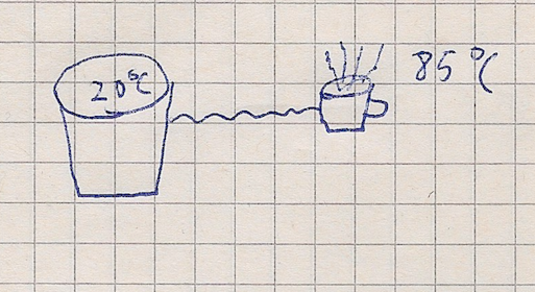
\includegraphics[width = \textwidth]{Zeichnungen/18.pdf}
  \caption{Zwei Systeme mit unterschiedlicher Temperatur.}
  %\label{fig:Bild}
\end{figure}
\paragraph{Kelvin:} Es gibt keinen zyklischen thermodynamischen Prozess, dessen einziger Effekt ist, einem Wärmereservoir Wärme zu entziehen  und diese völlig in Arbeit zu verwandeln.

% \begin{figure}[H]
%   \centering
%   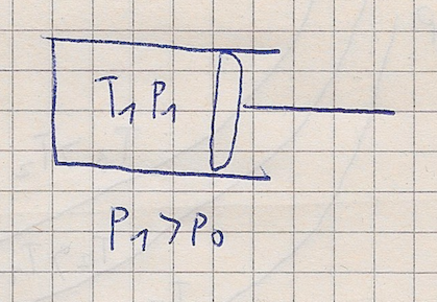
\includegraphics[width = \textwidth]{Zeichnungen/19.pdf}
%   \caption{Kolben.}
%   %\label{fig:Bild}
% \end{figure}
\begin{figure}
\centering
\begin{tikzpicture}
            \draw (0,1) rectangle (3, 2.5)
             (2,1) rectangle (2.5, 2.5)
             (2.5, 1.7) rectangle (6, 1.8)
             (1,1.75) node {$T V P_1$}
             (1, 0) node {$P_1 > P_0$};
\end{tikzpicture}
\caption{Kolben}
\end{figure}
\paragraph{Clausius:} Es gibt keinen zyklischen thermodynamischen Prozess, dessen einziger Effekt es ist Wärme von einem kalten Reservoir in ein wärmeres zu bringen. (Perpetuum Mobile 2. Art)  
\begin{itemize}
    \item Clausius $\Rightarrow$ Kelvin
    \item Wenn Kelvin falsch $\Rightarrow$ Clausius falsch
    \item entziehe Reservoir Wärme $\Rightarrow$ Arbeit
    
\end{itemize}
\paragraph{Carnotprozess}
\begin{figure}[H]
  \centering
  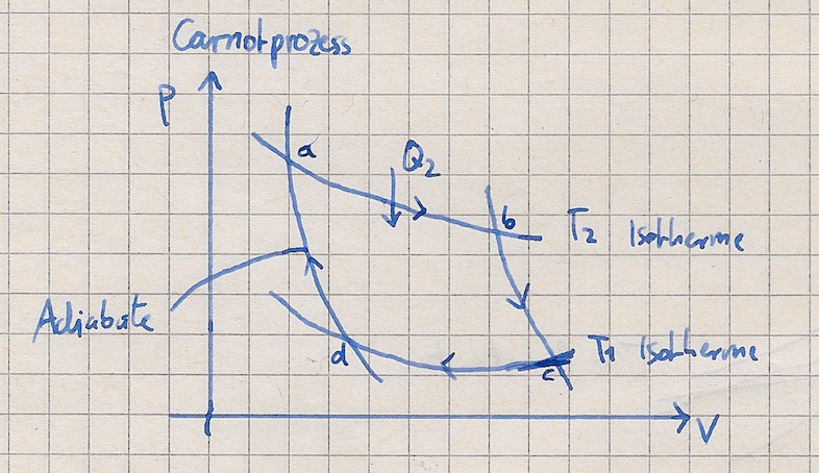
\includegraphics[width = \textwidth]{Zeichnungen/20.pdf}
  \caption{Der Carnotprozess.}
  %\label{fig:Bild}
\end{figure}
\begin{figure}[H]
  \centering
  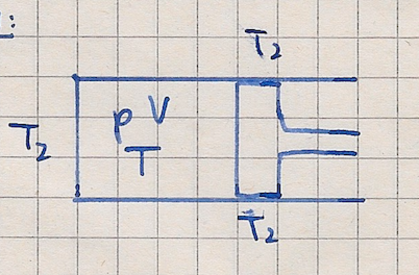
\includegraphics[width = \textwidth]{Zeichnungen/21.pdf}
  \caption{Kolben mit Temperaturangabe.}
  %\label{fig:Bild}
\end{figure}
\begin{figure}[H]
  \centering
  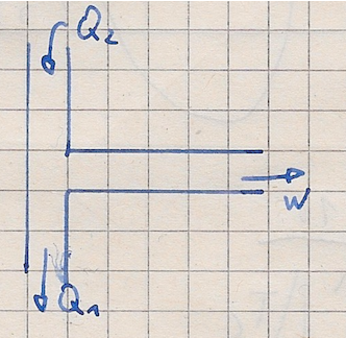
\includegraphics[width = \textwidth]{Zeichnungen/22.pdf}
  \caption{System mit Wärmeaufnahme und -abgabe und Arbeitabgabe.}
  %\label{fig:Bild}
\end{figure}
\begin{figure}
\centering
\begin{tikzpicture}
            \draw (0,0) rectangle (3,1.5)
             (2,0) rectangle (2.5, 1.5)
             (2.5, 0.7) rectangle (6, 0.8)
             (1,0.75) node {$P\ V\ T$}
             (1, -0.5) node {$T_2$}
             (-0.5, 0.75) node {$T_2$}
             (1, 2) node {$T_2$};
\end{tikzpicture}
\end{figure}

\begin{figure}
\centering
\begin{tikzpicture}
            \draw (0,0) -- (0,3)
                  (0.2, 0) -- (0.2, 1.4) -- (1.5,1.4)
                  (1.5, 1.6) -- (0.2, 1.6) -- (0.2, 3)
                  [->] (0.1, 0.5) -- (0.1, -0.1);
            \draw [->] (0.1, 3.1) -- (0.1, 2.5);
            \draw [->] (1.2, 1.5) -- (1.8, 1.5);
            \draw (0.5, 0) node {$Q_1$}
                  (0.5, 3) node {$Q_2$}
                  (2.5, 1.5) node {$W$};
\end{tikzpicture}
\end{figure}

\begin{align}
    \frac{pV}{T} &= N k_B\\
    P &= \frac{N k_\text{B} T}{V}
\intertext{Adiabaten immer steiler als Isotherme}
    \dif U &= \delta Q - \delta W\\
    &= T\dif S - p \dif V\\
    U &= \frac32 k_\text{B} N T\\
    \dif U&=0  \\
    \delta U &= T \dif S \\
    Q &= T_2 (S_b-S_a)\\
\intertext{Verrichtete Arbeit}
    \int p \dif V&= N k_B T_2 \int_a^b \frac{\dif V}{V}\\
    &= N k_B T \ln\left(\frac{V_b}{V_a}\right)\\
    (S_b - S_a) &= k_\text{B} N \ln \left(\frac{V_b}{V_a}\right)\\
\intertext{Adiabatische Expansion}
    \delta Q &= 0\\
    \dif U &= -p \dif V \\
    \Delta U &= \frac32 k_B N (T_2-T_1)\\
    \dif U &= \frac 3{2} k_\text{B} N \dif T = -p \dif V = -\frac{N k_\text{B} T}{V} \dif V\\
    \int_b^c \frac{\dif V}{V}&=-\frac 32 \frac{\dif T}{T}\\ 
    \ln\left(\frac{V^c}{V_b}\right) &= \ln\left(\frac{T^c}{T_b}\right)^{-3/2}\\
    V &= V_b \left(\frac{T}{T_b}\right)^{-3/2}\\
    V T^{\frac{3}{2}} &= \frac{V_b}{T_b^{-\frac 32}}= \text{const.} 
\intertext{Adiabatengleichung für ideales Gas}
    V^{\frac{2}{3}} T &= \text{const.} \\
    T V^{\varkappa-1} &= \text{const.}  \quad \varkappa = \frac{C_p}{C_V} = \frac{C_V+R}{C_V} = \frac{\frac{5}{2}}{\frac{3}{2}}\\
\intertext{ideales Gas}
    C_V&=\frac 32 R\\
    C_p-C_V&=R\\
    \varkappa&= \frac{5}{3}\\
    \Aboxed{ \varkappa -1 &= \frac{2}{3}}\\
    \Aboxed{\dif U &=0 \quad \text{Gesamtprozess}}
\end{align}
\begin{figure}[H]
  \centering
  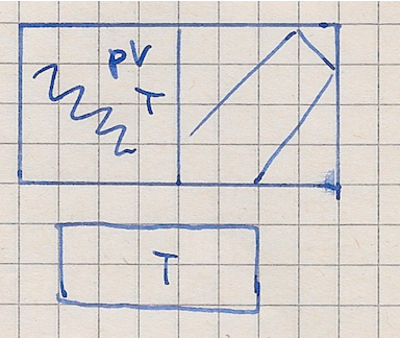
\includegraphics[width = \textwidth]{Zeichnungen/23.pdf}
  \caption{Zwei Systeme.}
  %\label{fig:Bild}
\end{figure}
\begin{align}
    \text{Wirkungsgrad} \quad  \eta &= \frac{\text{geleistete Arbeit}}{\text{aufgenommene Wärme}}\\
    \eta &= \frac{Q_2 - Q_1}{Q_2} = 1- \frac{Q_1}{Q_2} \quad Q_1 = 0 \Rightarrow \text{bestmöglicher Prozess}
\end{align}
Zeige, dass dies so ist (Huang)
\begin{enumerate}
    \item Maschine X
    \item Carnotprozess C
    \item $\Rightarrow$ Beide zwischen $T_1$ und $T_2$
\end{enumerate}
\begin{figure}[H]
  \centering
  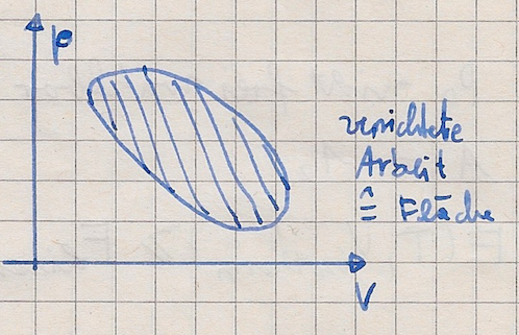
\includegraphics[width = \textwidth]{Zeichnungen/24.pdf}
  \caption{Verrichtete Arbeit in einem Kreisprozess.}
  %\label{fig:Bild}
\end{figure}
\begin{align}
    X \to W' \\
    C \to W  \\
    W_\text{total} &= N'W' - N W \\
    Q_\text{2, total} &= N' Q_2' - N Q_2 = 0\\
    Q_\text{1, total} &= N' Q_1' - N Q_1\\
    W_\text{total} &= N' W' - N W = \cancel{Q_\text{2, total}} - Q_\text{1, total} = - Q_\text{1,total} \\
    \underarrow{W_\text{total} > 0 }{\text{Widerspruch zu Kelvin}}\\
    \Aboxed{\Rightarrow W_\text{total}} \leq 0 \quad \text{\enquote{Unten wird Wärme abgegeben}}
\end{align}

\begin{align}
    N'&=\frac{Q_2}{Q_2'}  N\\
    Q_\text{1 total}&= N' Q_1' -N_1 Q_1 \geq 0\\
    \frac{Q_2}{Q_2'} N Q_1'-N_1 Q_1 &\geq 0 \quad \bigg \rvert \quad \frac{Q_2'}{N} \\
    Q_2 Q_1' &\geq Q_2' Q_1\\
    \frac{Q_1}{Q_2} &\geq \frac{Q_1'}{Q_2'}\\
    \Aboxed{1-\frac{Q_1}{Q_2} &\geq 1- \frac{Q_1'}{Q_2'}}\\
    \eta_c &\geq \eta_x 
\end{align}
\begin{figure}[H]
  \centering
  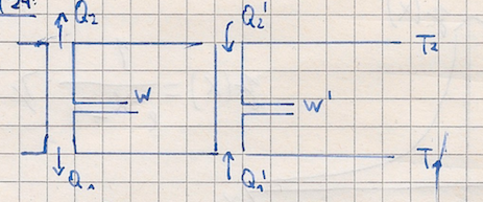
\includegraphics[width = \textwidth]{Zeichnungen/24b.pdf}
  \caption{???.}
  %\label{fig:Bild}
\end{figure}

Alle Carnotmaschinen die zwischen $T_1$ und $T_2$ \enquote{laufen} haben den gleichen Wirkungsgrad. Unabhängig von Arbeitsstoff und Konstruktion.
Möglichkeit die Temperatur materialunabhängig zu definieren.
\begin{align}
    \frac{Q_2}{Q_1}&=f(T_1,T_2)   & \frac{Q_2}{Q_1}&=\frac{\theta(T_2)}{\theta (T_1)} \\
    \delta Q &= C_V \dif T + \delta W & C_V &= \pdif{U}{T} \\
    \dif S &= \frac{\delta Q}{T}=C_V \frac{\dif T}{T} +\frac{R \dif V}{V} \\
 \text{(vollständiges Differential)}
  \end{align}

\begin{figure}[H]
  \centering
  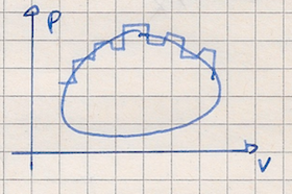
\includegraphics[width = \textwidth]{Zeichnungen/25.pdf}
  \caption{Mögliche Stufenform im p-V-Diagramm.}
  %\label{fig:Bild}
\end{figure}
\begin{align}
    S(T,V)&=C_V \int_{T_0}^T \frac{\dif T_0}{T} + R \int_{V_0}^V \frac{\dif V}{V}\\
    &= C_V \ln\left(\frac{T}{T_0}\right) + R \ln\left(\frac{V}{V_=}\right)\\ 
    &= \ln\left(\left(\frac{T}{T_0}\right)^{C_V} \left(\frac{V}{V_0}\right)^R \right)\\
    &= \ln\left( \left(\frac{T}{T_C}\right)^{C_V} \left(\frac{V}{V_0}\right)^{C_p-C_V}\right) \\
    \oint \frac{\delta Q}{T} &= 0 \quad \text{reversibel}
\end{align}
\section{Ideale Quantengase}
\subsection{Ideales Fermigas}

\begin{align}
    H &= \sum_j \epsilon_j  \hat n_j 
\end{align}
Freies Teilchen (Raum, Festkörper) 
\begin{align}
    \epsilon_{\vec k, \sigma} &= \frac{\hbar^2 \vec k^2}{2m^*} +\frac12 g^* \mu_B \sigma |\vec B| \\
\intertext{Großkanonische Zustandssumme}
    Z_\text{gk} &= Tr[e^{-\beta(\hat H - \mu \hat N)}] \\
\intertext{Kanonische Zustandssumme}
    Z_k &= \Tr[\e^{-\beta \hat H}]_{N = \text{const.}} \\
\intertext{Besetzungszahlbasis:}
    \Ket{n_1,n_2,...,n_j,...} \\
\text{Fermion:} \quad n_j  &= 0,1 \\
\text{Boson:} \quad n_j &= 0,1,2,...  \quad \in \mathbb{N}_0\\
    \hat n_j \Ket{n_1, ... n_j, ...} &= n_j \Ket{n_1, ....} \\
    N &= \sum_{j=1}^{\infty} n_j \qquad
    \hat N = \sum_{j=1}^{\infty} \hat n_j \qquad
    [\hat n_i, \hat n_j] = 0\\
    \hat F &= \e^{-\beta(\hat{H}-\mu \hat{N})} = \e^{-\beta \left(\sum_{j=1}^{\infty} (\epsilon_j - \mu) \hat{n}_j \right)} \\
    &= \prod_{j=1}^{\infty} \left( \e^{-\beta(\epsilon_j-\mu) \hat{n}_j} \right) = \prod_{j=1}^{\infty} F_j((\hat n)_j) \\
    \Tr[\hat F]_{\text{gk}}&= \Tr\left[\prod_{j=1}^\infty F_j(\hat n_j)\right]_{\text{gk}}\\
    &=\sum_{\{n_j=0,1\}} \Bra{n_1,n_2,...,n_j,...}\underbrace{\prod_{j=1}^\infty F_j(\hat n)\Ket{n_1,...,n_j,...}}_{\prod_{j=1}^\infty F_j(n_j)}\\
    &=\sum_{\{n_j=0,1\}} \prod_{j=1}^{\infty}F_j(n_j)\\
    &= \prod_{j=1}^\infty (F_j (0) + F_j (1))\\
    \Rightarrow Z_\text{gk} &= \prod_{j=1}^\infty \underbrace{(1+\e^{-\beta(\epsilon_j-\mu)})}_{Z_j} = \prod_{j=1}^\infty Z_j\\
    \Braket{\hat n_j} &= \frac1{Z_{\text{gk}}} \Tr[\e^{-\beta H -\mu\hat N} \hat n_j] = \frac{\cancel{\prod_{n \neq j}^{\infty} Z_n} (0 + \e{-\beta (\epsilon_j - \mu )})}{\cancel{\prod_{n=1}^\infty} \underarrow{Z_n}{Z_j}}
\end{align}
\begin{figure}[H]
  \centering
  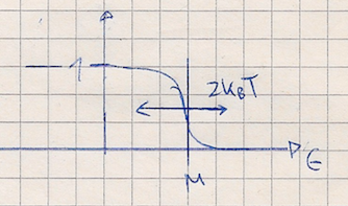
\includegraphics[width = \textwidth]{Zeichnungen/26.pdf}
  \caption{Energie.}
  %\label{fig:Bild}
\end{figure}
\begin{align}
    &= \frac{\e^{-\beta(\epsilon_j - \mu)}}{1+e^{-\beta(\epsilon_j - \mu)}} = \frac{1}{1 + e^{\beta(\epsilon_j - \mu)}+1} = \underarrow{f(\epsilon_j-\mu)}{\text{Fermi-Funktion}} 
\end{align}
\paragraph{Großkanonisches-Potential}
\begin{align}
    \Phi(T,\mu)=-\frac{1}{\beta}\ln Z_{\text{gk}}=-k_B T\sum_{j=1}^{\infty} \ln\left(1+\e^{-\beta(\epsilon_j-\mu)}\right)
\end{align}
\paragraph{Teilchenzahl}
\begin{align} 
    N &= -\pdif{\Phi}{\mu} = \frac{1}{\cancel{\beta}} \sum_{j=1}^{\infty} \underbrace{\frac1{1+\e^{-\beta(\epsilon_j - \mu)}} \cancel{\beta} \e^{-\beta (\epsilon_j - \mu)}}_{f(\epsilon_j - \mu)} \\
    N&=\sum_{j=1}^\infty \Braket{\hat n_j}=\sum_{j=1}^\infty f(\epsilon_j-\mu)
\end{align}
\paragraph{Innere Energie}
\begin{align}
    U = \Braket{\hat{H}} = \sum_{j=1}^{\infty} \epsilon_j f(\epsilon_j - \mu) = - \pdif{\Phi}{\beta}\biggr\rvert_{\beta \mu= \text{const.}}
\end{align}
\paragraph{Entropie}
\begin{align}
    S &= -\pdif{\Phi}{T} = \left(\pdif{\Phi}{\beta}\right) \left(\pdif{\beta}{T}\right) = k_\text{B} \beta^2 \pdif{\Phi}{\beta} \\  
    \pdif{\Phi}{\beta}&= \frac{1}{\beta^2} \ln Z_{\text{gk}}-\frac{1}{\beta} \sum_j \pdif{}{\beta} \ln Z_j\\
    &=\frac{1}{\beta^2} \ln Z_\text{gk}-\frac{1}{\beta^2} \sum_j \frac{1}{1+\e^{-\beta(\epsilon_j-\mu)}} \beta \left(-(\epsilon_j -\mu)\right) \e^{-\beta}\\
    &= \frac{1}{\beta^2} \ln Z_\text{gk} + \frac{1}{\beta^2} \sum_j \beta(\epsilon_j - \mu) f_j \\
    1-f_j &= 1- \frac1{\e^{\beta (\epsilon_j - \mu }+1} = \frac{\e^{\beta (\epsilon_j - \mu }}{\e^{\beta (\epsilon_j - \mu } + 1} = \frac1{Z_j}\\
    \ln(Z_j)&=-\ln(1-f_j)\\
    \beta(\epsilon_j-\mu) &= \ln(\underbrace{\e^{-\beta(\epsilon_j-\mu)}+1}_{\sfrac{1}{f_j}}-1)=\ln\left(\frac{1-f_j}{f_j}\right)=\ln(1-f_j)-\ln f_j\\
    S&=k_B\sum_{j=1}^\infty \ln(Z_j)+\beta(\epsilon_j-\mu) f_j\\
    &=k_B \sum_{j=1}^\infty \left(\left(-\ln(1-f_j)\right)+\left(\ln(1-f_j)-\ln f_j\right)f_j\right)\\
    &=-k_B\sum_{j=1}^\infty\left(\underbrace{f_j}_{P_j^1}\ln f_j +\underbrace{(1-f_j)}_{P_j^0}\ln(1-f_j)\right)\\
    S&= -k_B\sum_{j=1}^\infty \left( P_j^0 \ln P_j^0 + P_j^1 \ln P_j^0 \right) \checkmark
\end{align}

Dispersion eines freien Teilchens 
\begin{align}
    \epsilon_{\vec k} &= \frac{\hbar^2 k^2}{2m}\\
    \Rightarrow U&=\sum_j \epsilon_j f(\epsilon-\mu)=\sum_{\vec k \sigma} \epsilon_{\vec k \sigma} \underarrow{f}{\text{Fermifunktion hängt nur von der Energie ab!}}(\epsilon_{\vec k \sigma}-\mu) \\
\intertext{Zustandsdichte:}
    \rho_\sigma &= \frac1V \sum_{\vec k} \delta(\epsilon-\epsilon_{\vec k, \sigma}) \\
    \Rightarrow \Aboxed{U &= \sum_\sigma V \int_{-\infty}^{\infty} \symup{d} \epsilon \rho_\sigma (\epsilon) f(\epsilon - \mu)}\\
    N &= \sum_j f(\epsilon_j - N ) = \underarrow{2V}{\sum_\sigma} \int_{-\infty}^{\infty} \dif \epsilon \ \rho(\epsilon) f(\epsilon-\mu)\epsilon \\
    \Aboxed{n &= \frac{1}{v}=2 \int_{-\infty}^{\infty} \dif \epsilon \rho(\epsilon) f(\epsilon-\mu)} \\ &\text{Imp\emph{lizite?} Gleichung für $\mu$ bei kanonischer Rechnung} \\
    n &= \frac1v = \frac NV
\end{align}
\begin{figure}[H]
  \centering
  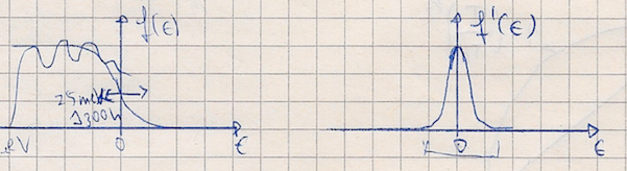
\includegraphics[width = \textwidth]{Zeichnungen/27.pdf}
  \caption{.}
  %\label{fig:Bild}
\end{figure}
\begin{align}
\intertext{Integrale vom Typ:}
    \int_{-\infty}^\infty \dif \epsilon f(\epsilon-\mu) I(\epsilon) &= \underbrace{\cancel{f(\epsilon)k(\epsilon)\biggr\rvert_{-\infty}^\infty}}_{=0} + \int_{-\infty}^\infty \dif \epsilon \left(-\pdif{f}{\epsilon}\right) K(\epsilon)\\
    K(\epsilon) &= \int_{-\infty}^{\epsilon} \dif \epsilon' I(\epsilon')\\
    -\pdif{f}{\epsilon} &=-\pdif{}{\epsilon}\left(\frac{1}{\e^{-\beta(\epsilon-\mu)}+1}\right) \\
    &=\frac{1}{\e^{-\beta(\epsilon-\mu)}+1} \frac{1}{\e^{-\beta \epsilon-\mu)}+1} \beta \e^{\beta(\epsilon-\mu)}\\
    &=\beta f(\epsilon -\mu)f(-(\epsilon-\mu))
\end{align}

\paragraph{Taylor-Entwicklung}
\begin{align}
    K(\epsilon)&=K(\mu)+\sum_{n=1}^{\infty} \frac{1}{n!}(\epsilon-\mu)^n \frac{\dif^n K(\epsilon)}{\dif \epsilon^n}\biggr\rvert_{\epsilon=\mu} \\
    \Aboxed{\int_{-\infty}^{\infty} \dif \epsilon f(\epsilon - \mu) I(\epsilon) &= \int_{-\infty}^{\mu} \dif \epsilon I(\epsilon) + \sum_{n=1}^{\infty} \frac{1}{n!} \frac{\dif^{n-1}I(\epsilon)}{\dif\epsilon^{n-1}}\biggr\rvert_{\epsilon = \mu} \underbrace{\int_{-\infty}^\infty \dif \epsilon \left(-\pdif{f}{\epsilon} \right) (\epsilon - \mu)^\mu}_{=0 \text{ für n ungerade}}}
    \intertext{Sommerfeld-Entwicklung}
\end{align}

Zustandsdichte
\begin{align}
    \rho(\epsilon) &= \frac{1}{v}\sum_{\vec k} \delta(\epsilon-\epsilon_{\vec k \epsilon})  \qquad \quad \text{z.B.} \epsilon_{\vec k}=\frac{\hbar^2 k}{2 m}\\
    %\int_{-\infty}^\infty \dif \epsilon f(\epsilon-\mu)I(\epsilon)=\int_{-\infty}^\mu \dif \epsilon I(\epsilon)+\sum_{n=1}^\infty \frac{1}{n!}
    %\frac{\dif^{n-1}I(\epsilon)}{\dif\epsilon^{n-1}}\biggr\rvert_{\epsilon = \mu} \underbrace{\int_{-\infty}^\infty \dif \epsilon \left(-\pdif{f}{\epsilon} \right) (\epsilon - \mu)^\mu}_{=0 \text{für n ungerade}}
    \int_{-\infty}^\infty (\epsilon - \mu)^{2n} \left(-\pdif{f}{\epsilon}\right) &= \underbrace{\beta \int_{-\infty}^\infty \dif \epsilon}_{\dif x}(\beta(\epsilon - \mu))^{2n} \frac{\e^{\beta (\epsilon-\mu)}}{(\e^{\beta (\epsilon-\mu)}+1)^2} \frac{1}{\beta^{2n}} \\
    &= (k_B T )^{2n}  \int_{-\infty}^\infty \dif x x^{2n} \frac{\e^{x}}{(\e^{x}-1)^2} = (k_B T)^{2n} A_{2n}\\
    f(\epsilon) = \frac1{\e^{\beta \epsilon}+1} \qquad x &= \beta(\epsilon - \mu) \qquad \dif x = \beta \dif \epsilon 
\end{align}
%
\begin{figure}[H]
  \centering
  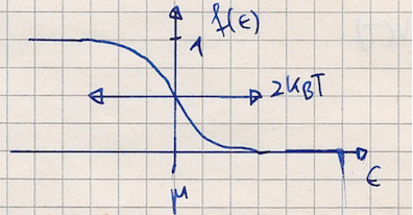
\includegraphics[width = \textwidth]{Zeichnungen/28.pdf}
  \caption{.}
  %\label{fig:Bild}
\end{figure}
%
\paragraph{$\Rightarrow$ Riemannsche $\zeta$-Funktion} 
\begin{align}
    \tdif{}{\lambda} \left(\frac{1}{\e^{\lambda x}+1}\right) &= - \frac{x \e ^{\lambda x}}{(\e^{\lambda x} +1)^2} \\
    A_{l = 2n} &= \int_{-\infty}^{\infty} \dif x x^l \frac{\e^x}{\left(\e^x + 1 \right)^2} = -2 \tdif{}{\lambda} \underbrace{\left[ \int_{-\infty}^{\infty} \dif x x^{l-1} \frac1{\e^{\lambda x} + 1} \right]}_{u = \lambda x \quad \dif u = \lambda \dif x}\\
    &=-2\tdif{}{\lambda}\left[\frac{1}{x^l}\int_0^\infty \dif u \frac{u^{l-1}}{\e^u + 1}\right]
    = 2l \int_{0}^\infty \dif U \frac{U^{l-1}}{\e^{U}+1}
\end{align}

\paragraph{Riemannsche $\zeta$-Funktion: Integraldarstellung}
\begin{align}
    \zeta (l) &= \frac1{(1-2^{l-1})\Gamma(l)} \int_0^\infty \dif U \frac{U^{l-1}}{\e^U +1} & \\
    A_{l=2n}&=2\underbrace{(2n)\underbrace{\Gamma(2n)}_{(2n-1)!}}_{(2n)!} \left(1-2^{1-2n}\right)\zeta(2n) & \Rightarrow A_0&=2(1-2^1)\underarrow{\zeta(0)}{-\frac12}=1\\
    &&   A_2&=2 2!(1-2^{1-2})\underarrow{\zeta(2)}{\frac{\pi^2}{6}}=\frac{\pi^2}{3}\\
\end{align}
\begin{align}
    I(\epsilon) &= \rho(\epsilon) \\
    n &= \frac1v = \underarrow{2}{\text{Spin}}\left[\int_{- \infty}^\mu \dif \epsilon \rho (\epsilon) + \frac{1}{2!} \rho' (\mu) (k_B T)^2 \frac{\pi^2}{3} + \mathcal O((k_B T)^4)\right]  \label{eqn:zeile117}\\
    U&=\frac{U}{V}=2\int_{-\infty}^\mu \dif \epsilon \ \epsilon \rho(\epsilon) +\tdif{}{\epsilon}\biggr\lvert_{\epsilon=\mu} (k_B T)^2 \frac{\pi^2}{3}+... \\
\intertext{Energiedichte $\quad \Phi(\epsilon) = \rho(\epsilon) \epsilon$}
\end{align}
\begin{align}
    U &= 2 \int_{-\infty}^{\infty} \dif \epsilon \ \epsilon \rho(\epsilon) + [\rho(\mu) + \mu \rho'(\mu)] (k_\text{B} T)^2 \frac{\pi^2}{3} + ... \label{eqn:zeile121}\\
    \eqref{eqn:zeile121}  \stackrel{T \to 0}{\rightarrow} \quad U_0 &= 2 \int_{-\infty}^{\mu_0} \dif \epsilon\ \epsilon \rho(\epsilon)\\
    \eqref{eqn:zeile117}  \stackrel{T \to 0}{\rightarrow}  \quad \frac1v &= 2 \int_{-\infty}^{\mu_0} \dif \epsilon \rho(\epsilon)\\
    \eqref{eqn:zeile117}-\eqref{eqn:zeile117} \text{bei $T=0$}:  0&=\left[\int_{\mu(0)}^{\mu(T)}\dif \epsilon \rho(\epsilon) +\frac{\pi^2}{6}\rho'(\mu)(k_B T)^2 +...\right]\\
    &\Rightarrow \mu(T)-\mu_0 \approx (k_B T)^2\\
    0 &\approx \rho(\mu_0)[\mu(T)-\mu_0]+\frac{\pi^2}{6}\rho'(\mu_0)(k_B T)^2+...\\
    \Aboxed{\mu(T) &= \mu_0 - \frac{\pi^2}{6} \frac{\rho'(\mu)}{\rho(\mu)} (k_B T)^2}
\end{align}
\begin{figure}[H]
  \centering
  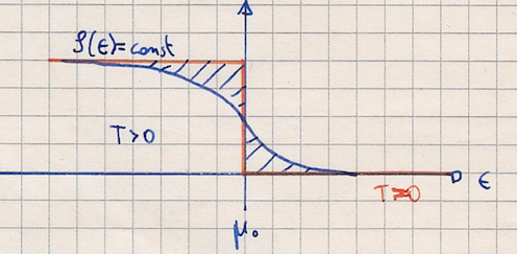
\includegraphics[width = \textwidth]{Zeichnungen/29.pdf}
  \caption{Übergang zur Sprungfunktion.}
  %\label{fig:Bild}
\end{figure}
\begin{align}
    \epsilon_k&=\frac{\hbar^2 k^2}{2 m} \qquad 3D:  \quad \rho \approx \sqrt{\epsilon} \quad \rho'(\mu)>0 
\end{align}
\begin{figure}[H]
  \centering
  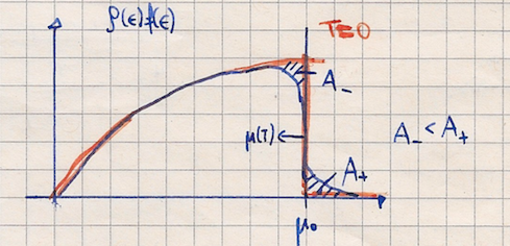
\includegraphics[width = \textwidth]{Zeichnungen/30.pdf}
  \caption{.}
  %\label{fig:Bild}
\end{figure}
\begin{align}
    U(T)-\frac{U(T=0)}{V} &= 2\left[\underarrow{(\mu(T)-\mu_0)}{\cancel{-\frac{\pi^2}{6}\frac{\rho'(\mu)}{\rho(\mu)}(k_B T)^2}}\mu_0\rho(\mu_0))+\frac{\pi^2}{6} (\rho(\mu_0)+\cancel{\mu_0 \rho'(\mu_0)})(k_B T)^2+...\right] \\
    &= \frac{\pi^2}{3} \rho(\mu_0) (k_B T)^2 
\end{align}

\paragraph{Spezifische Wärme}

\begin{align}
    C_V &= \pdif{U}{T}[V = \text{const.}] = V \pdif{}{T} [U(T)- U (0)] = 2V \frac{\pi^2}{3} \rho(\mu_0) k_B^2 T = \gamma T\\
\intertext{Gamma-Koeffizient: $\gamma = 2 U_B^2 \rho(\mu_0)\frac{\pi^2}{3}V$}
    C_v &\propto T \quad \text{und verschwindet für $T \to 0$}\\
    \sum_{\vec k} \underarrow{I(\epsilon_{\vec k})}{\delta(\epsilon-\epsilon_k) \epsilon=\frac{\hbar^2}{2m}k^2}&=\frac{V}{(2\pi)^d} \int \dif^d k \quad \quad \int\dif^d k=\int_0^\infty \dif k k^{d-1} O_d\\
    \rho(\epsilon) &= 
    \begin{cases}
    a\frac{1}{\sqrt{\epsilon}} &d=1\\
    a   &d=2\\
    a\sqrt{\epsilon}  &d=3 
    \end{cases} \qquad = a_x\epsilon^x
\end{align}
\begin{align}
    \Psi(T, N, V) &= - \frac1\beta \ln(Z_\text{gk}) = - 2 k_B T V \int_{-\infty}^{\infty} \dif \epsilon \rho(\epsilon) \ln(1 + \e^{-\beta(\epsilon-\mu)})\\
    N &= \sum_{??G} f(\epsilon_k - \mu) = 2 V \int_{-\infty}^\infty \dif \epsilon f(\epsilon-\mu) \rho(\epsilon)\\
    \int\dif\epsilon\rho(\epsilon)&=a \int \dif \epsilon \epsilon^x =\frac{a}{1+x}\epsilon^{1+x}=\frac{\epsilon}{1+x}\rho(\epsilon)
\intertext{Druck: (Zustandsgleichung)}
    p&=-\pdif{\Phi}{V}=2 k_B T \int_{-\infty}^\infty \dif \epsilon \rho(\epsilon) \ln(1+\e^{-\beta(\epsilon-\mu)}) \\
    &=2k_B T \left[\frac{\epsilon}{1+x}\rho(\epsilon) \ln(1+\e^{-\beta(\epsilon-\mu)})\right]_{-\infty}^\infty \\ 
    &\quad -\frac{1}{1+\epsilon}\int_{-\infty}^\infty \dif \epsilon \epsilon \rho(\epsilon) \underbrace{\frac{\beta \e^{-\beta(\epsilon-\mu)}}{1+\e^{-\beta(\epsilon-\mu)}}}_{-\beta f(\epsilon-\mu)}\\
    p &= \frac1{1+x} \underbrace{2 \int_{-\infty}^{\infty} \dif \epsilon \rho(\epsilon) \epsilon f(\epsilon - \mu)}_{\frac{U}{V}}\\
    \Rightarrow \Aboxed{pV &= \frac1{1+x}}\\
    \text{3D: } x &= \frac12 \\
    pV & =\frac32 U\\
    \intertext{ideales Gas: $U = \frac32 N k_B T$}
\end{align}

\paragraph{Grundzustand}

\begin{align}
    N &= \underarrow{2}{\text{Spin}} \frac{V}{\underbrace{(2 \pi)^3}_{d = 3}} \frac{4 \pi}{3} k_F^3\\
    k_F^2&=\left(\frac{3N\pi^2}{V}^{\frac23}\right)\\
    \Rightarrow \underarrow{\epsilon_F}{\text{Fermienergie}}&=\frac{\hbar^2}{2m}\left(\frac{3N\pi^2}{V}\right)^{\frac23}
\end{align}

\subsubsection{Klassischer Grenzfall}

\begin{align}
    \text{bisher: } T &\to 0 (\beta \to \infty)\\
    \text{jetzt: } T &\to \infty (\beta \to 0)\\
\intertext{Frage: Geht das Fermigas in das klassische ideale Gas über?}
    \text{Beispiel: } \epsilon_{\vec k} &= \frac{\hbar^2 k^2}{2m} \qquad 3D\\
    \Phi(T,\mu,V) &= - \frac{1}{\beta} \ln(Z_\text{gk}) = - k_\text{B} T \frac{2 V}{(2 \pi)^3} \int \dif^3k \ln \left( 1 + z \e^{-\beta \frac{\hbar^2 k^2}{2m}}  \right)\\
    z&=\e^{\beta \mu} \qquad \text{Fugazität} \\
    x &= k \sqrt{\frac{\beta \hbar^2}{2m}}; \quad \dif x = \hbar \sqrt{\frac{\beta}{2m}} \dif k \\ 
    \Phi &= - k_\text{B} T \frac{2 V}{(2 \pi)^3} \left(\sqrt{\frac{2m}{\beta \hbar^2}}\right)^3 4 \pi \int_0^\infty \dif x\ x^2 \ln(1 + z \e^{-x^2})\\
\intertext{Thermische de-Broglie-Wellenlänge:}
    \lambda_T(T) &= \frac{2 \pi \hbar}{\sqrt{2 \pi m k_\text{B}}} = \sqrt{\frac{2\pi \beta \hbar^2}{m}} \\
    \Phi&=-k_\text{B} \frac8{\sqrt{\pi}}\frac{V}{\lambda_T^3}
    \int_0^\infty \dif x\ x^2 \ln(1+\underbrace{z\e^{-x^2}}_{y})
\intertext{Taylorreihe:}
    \ln(1+y) &= \sum_{n=1}^{\infty} (-1)^{n+1} \frac{y^k}{k} \quad |y| \leq 1 \\
    \int_0^\infty \dif x \ln \left( 1 + z e^{-x^2} \right) x^2
    & =\sum_{n=1}^\infty (-1)^{k+1}\frac{z^n}{n} \int_0^\infty \dif x \underbrace{x^2 e^{-nx^2}}_{-\tdif{}{n} \e^{nx^2}} \\
    &= \sum_{n=1}{\infty} (-1)^{n+1} \frac{z^n}{n} (- \tdif{}{n} \frac{\sqrt{\pi}}{2} \underarrow{n^{-\frac12}}{-\frac12 n^{-\frac32}}) \\
    &= \frac{\sqrt{\pi}}{4} \sum_{n=1}^\infty (-1)^{n+1} \frac{z^n}{n^{\frac{5}{2}}} = \frac{\sqrt{\pi}}{4} f_{\frac{5}{2}}(z) \\
    f_{\frac32}(z)&=z\tdif{}{z} f_{\frac52}(z)=z\sum_{n=1}^\infty (-1)^{n+1}\frac{\cancel{n}z^{n-1}}{n^{\cancel{\frac52}\frac32}} =\sum_{n=1}^\infty (-1)^{n+1} \frac{z^{n}}{n^{\frac32}} \\
    \Rightarrow \Phi(T, \mu, V) &= - k_B T \frac{2V}{\lambda_T^3 f_{\frac52(z)}}\\
\intertext{Zustandsgleichung:}
    p &= -\pdif{\Phi}{V} = k_\text{B} T \frac{1}{{\lambda_T}^3} f_{\frac{5}{2}}(z) \\
    N &= z \tdif{}{z} \ln(Z_{\text{gk}}) = 2 V z  \tdif{}{z} \frac1{\lambda^3} f_\frac52 (z)\\
    \Aboxed{N &= \frac{2V}{\lambda_T^3} f_\frac{5}{2}} \label{eqn:zeile205} \\
    \text{Für } \beta \to 0 (t \to \infty) \quad &\Rightarrow \lambda_T \to 0 \quad \Rightarrow \frac1{\lambda_T} \to \infty \\
    &\text{Aus} \stackrel{\eqref{eqn:zeile205}}{\rightarrow} f_{\frac52}(z)\rightarrow 0 , z \rightarrow 0\\
    z\rightarrow 0: f_{\frac{3}{2}(\frac{5}{2})}(z)&\approx z-\frac{z^2}{2^{\frac{3}{2}(\frac{5}{2})}}\\
\intertext{Aus \eqref{eqn:zeile205}}
    \text{0. Näherung:} z_0 &= \frac{n \lambda_T^3}{2} \quad ; n= \frac NV \\
    \frac{n \lambda_T}{2} &= f_\frac32 (z) = z_0 = z_1 \left(1 - \frac{z_0}{2^\frac32}\right)\\ 
    z_1 &\approx \frac{z_0}{1-\frac{z_0}{2^\frac{3}{2}}} \approx z_0\left(1+\frac{z_0}{2^{\frac{3}{2}}}\right) \\
    pV &= \frac{k_\text{B}T}{\lambda_T^3} \frac{2V}{N} \left[ \underarrow{z}{z_1} - \underarrow{z^2}{z_0^2}\frac{1}{2^{\frac{5}{2}}} + \mathcal O(z^3)\right]\cdot N\\
    &= k_B T N \cancel{\frac1z_0} \cancel{z_0} \left[1+ \frac{z_0^2}{2^\frac32} -\frac{z_0}{2^\frac52} + O(z_0^2)\right]\\ 
    pV&=k_\text{B}TN\left[\underarrow{1}{\text{Ideales Gas}\hspace{2cm}}+\underarrow{\frac{n \lambda_T^3}{2}\frac{1}{2^{\frac52}}}{\hspace{2cm}\text{Quantenkorrekturen}}+O(z_0^2)\right]
\end{align}
\subsection{Das ideale Bose-Gas}
\begin{align}
    H&=\sum_{\vec k} \epsilon_{\vec k} \hat n_k=\sum_{\vec k}  \epsilon_{\vec n}  b^\dagger_k b_k \\
    [b_{\vec k}, b_{\vec k'}^\dagger] &= \delta_{\vec k, \vec k'} \quad ; \epsilon_k=\frac{\hbar^2 k^2}{2m}\\
    \Tr\left[\prod_{\vec k} F_k(\hat n_k)\right]_{\text{Fock-Raum}} &= \prod_K \Tr\left[F_{\vec k}(\hat n_k)\right]\\
    Z_{\vec k} &= \Tr \left[ \e^{-\beta(\epsilon_{\vec k} - \mu)\hat n_k} \right] = \sum_{n=0}^\infty[\e^{\beta(\epsilon_k-\mu)}]^k = \frac1{1-e^{-\beta (\epsilon_k - \mu)}} \\
    \Braket{\hat n_k} \frac{1}{z_k}\Tr[\hat n_k \e^{-\beta(\epsilon_k-\mu)\hat n_k}]
    &= \frac{\e^{-\beta (\epsilon_{\vec k}- \mu)}}{1- \e^{-\beta (\epsilon_{\vec k}- \mu)}} = \frac{1}{\e^{-\beta (\epsilon_{\vec k}- \mu)}-1} = \underarrow{g}{\text{Bose-Funktion}}(\epsilon_{\vec k} - \mu)\\
    \Braket{n}&=-\frac{1}{\beta}\pdif{\ln(z)}{\epsilon}
\end{align}
\begin{align}
\intertext{Thermodynamisches Potential}
    \Phi(T, \mu, N) &= k_\text{B} T \sum_k \ln(1-\e^{-\beta \epsilon_k -\mu}) \\
    N & = \sum_{\vec k} g(\epsilon_{\vec k} - \mu) \qquad S = \pdif{\Phi}{T}
\end{align}
\begin{figure}[H]
  \centering
  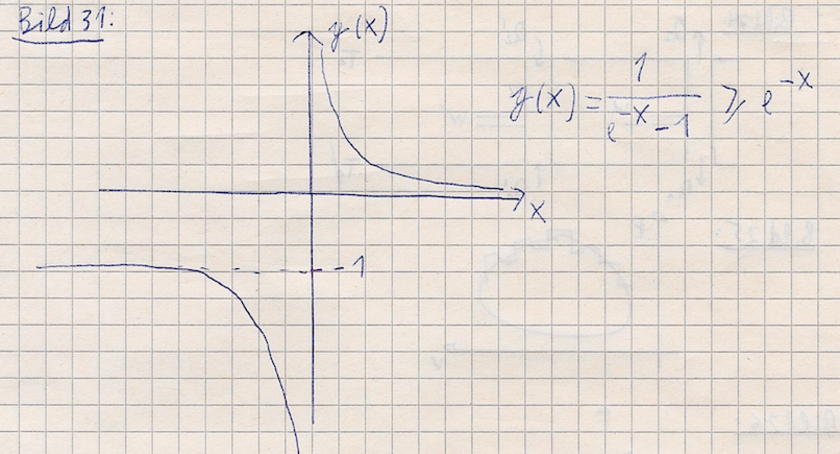
\includegraphics[width = \textwidth]{Zeichnungen/31.pdf}
  \caption{.}
  %\label{fig:Bild}
\end{figure}
\begin{align}
\intertext{Bose-Funktion singulär bei $\beta x \to 0$}
    \e^{\beta x} \approx 1 + \beta x \\
    \Rightarrow g(x) &= \frac{1}{e^{\beta x} -1} \approx \frac{1}{1+\beta x -1} \approx \frac{1}{\beta x} \\ 
    g(x) &< 0 \quad \text{für} \quad x < 0 \\ 
    g(x) &= \frac{1 - \e^{\beta x} + \e^{\beta x}}{\e^{\beta x} - 1} = -1 + \frac{\e^{\beta x}}{\e^{\beta x} -1} \to -1 - \e^{\beta x} \quad \text{für} \quad \beta x \to - \infty \\
    \text{Da }
    &\begin{drcases*}
     n_k= \Braket{\hat n_k} & $\geq 0$\\
     \text{und} \ \epsilon &$\geq 0$
    \end{drcases*} %hoffentlich klappt das 
    \Rightarrow \mu \leq 0\\
    N &= V \int_0^\infty \dif \epsilon \underarrow{\rho(\epsilon)}{a_q \epsilon^{\frac{d-2}{2}}} g(\epsilon-\mu)\geq V a \int_{0}^{\infty} \dif \epsilon \ \epsilon^{\frac{d}{2} - 1} \underbrace{\e^{-\beta(\epsilon - \mu)}}_{\e^{\beta \mu}} \e^{-\beta \epsilon} \frac{\beta^{\frac{d}{2}-1}}{\beta^{\frac{d}{2}-1}} \frac{\beta}{\beta} \\
    &= Va \beta^{-\frac{d}{2}}\e^{\beta\mu}\underbrace{\int_0^\infty \dif x \e^{-x} x^{\frac{d}{2}-1}}_{A} \\
    \Rightarrow - \beta \mu &\approx \ln(\beta^{-\frac{d}{2}}) \\
    \Rightarrow \mu &\approx -T \ln(T) \\
    \text{Für} \to 0  \quad \mu(T) &\to 0^- \\
    T \to 0 &\quad \epsilon_k = 0 \\
    N&=\underarrow{g_0}{\text{Grundzustand makroskopisch besetzt}}=\frac1{\e^{\beta(\epsilon-\mu)}-1} = \frac{z}{z-1} \quad z=\e^{\beta \mu} \\
    \Rightarrow \mu(T) &\approx-bk_\text{B}T\\
    \Rightarrow N &\approx \frac1{\e^b -1} \\
    b &\approx \ln \left( 1 + \frac1{N} \right) \approx \frac1{N} \\
    M_k&=\sum_{\vec k}(\epsilon_{\vec k}^k g(\epsilon-\mu)=g_0 \delta_{k,0}+\sum_{\vec k, \epsilon_{\vec k}g_0} (\epsilon_{\vec k})^k g(\epsilon-\mu)  
\end{align}
\paragraph{Ideales Bose-Gas}
\begin{align}
    %g(x)&=\frac{1}{\e^{\beta x-\mu}-1} \stackrel{\epsilon = 0}{=} \frac{1}{\frac{1}{z} -1} = \frac{z}{1-z} \\
\end{align}
\begin{itemize}
      \item $\lim{x\to0^+}g(x)\to \infty$
      \item Grundzustandsbesetzung kann makroskopisch werden $g(\epsilon)\propto O(N)$
      \item $g(\epsilon)=\Braket{n_\epsilon}\geq 0 \rightarrow$ schränkt die Wertemenge von $M$ ein
\end{itemize}
\begin{align}
    M_n &= \sum_{\vec k} (\epsilon_{\vec k})^n g(\epsilon_{\vec k})
    \underarrow{=}{\epsilon=0: \text{ Grundzustandsenergie}}
    g_0\delta_{n,0}+\sum_{\vec k,\epsilon_{\vec k}g_0} (\epsilon_{\vec k})^n g_k(\epsilon_{\vec k}-\mu)\\
    \Aboxed{N=M_0,&\quad U=M_1} \\
    \vec p&=\hbar \vec k\\
    M_n&= g_0\delta_{n,0}+\frac{V}{(2\pi\hbar)^d} O_d \int_0^\infty \dif p
    p^{d-1} \left(\frac{p^2}{2M}\right)^n \frac{1}{\frac{1}{z}\e^{\beta\frac{p^2}{2M}}-1 }\\
    O_d &= \frac{2\pi^{\frac{d}{2}}}{\Gamma(\frac{d}{2})} \quad \text{Oberfläche der $d$-dimensionalen Einheitskugel}\\
    &=\underbrace{...}_\text{Nebenrechnung}=g_0\delta_{n,0} + \frac{V}{{\lambda_T}^d}(k_\text{B}T)^n C_n^d g_{n+\frac{d}{2}}(z) \\
    g_n(z) &= \sum_{l=1}^\infty \frac{z^l}{l^k} = \Li_n(z) \qquad \text{Polylogarithmus}\\
    \text{Li}_1(z)&=-\ln(1-z)\\
    C_n^d&=\prod_{i=1}^n (n-i+\frac{d}{2}) \quad C_0^d =1\\
    \Rightarrow  \Aboxed{N &= \frac{z}{1-z} + \frac{V}{\lambda_T^d} g_{\frac d2}(z)}\\
    \Aboxed{U &= \frac{v}{{\lambda_T}^d} \cdot  \frac{d}{2} g_{1+\frac{d}{2}}(z) \kB T}  \\
\intertext{ Implizite Gleichung für M (oder $z=\e^{\beta M}$)}
\intertext{Zustandsgleichung}
    p&=-\pdif{\Phi(T,\mu,V)}{V} \quad \text{mit} \quad \Phi = -\frac{1}{\beta} \ln(Z_{\text{gk}}) = -\kB T \sum_k \ln(Z_k)\\
    \frac{p V}{\kB T} &= \frac{V}{(2 \pi \hbar)^d} O_d \int_0^\infty \dif p p^{d-1} \ln\left(1- z \e^{-\beta \frac{p^2}{2m}}\right) = \frac{V}{\lambda_T^d} g_{1+\frac{d}{2}} (z)\\
    \ln(1-z \e^{-\frac{\beta p^2}{2m}})&=-\sum_{l=1}^\infty \frac{1}{l}\left(z\e^{-\frac{\beta p^2}{2m}}\right)^l\\
    \Aboxed{pV &= \frac{2}{d}U} \qquad \text{identisch zum Fermigas} \\
    \lambda_T(T)&=\frac{2\pi \hbar}{\sqrt{2\pi M \kB T }} \\
    N_0 &= \frac z{1-z}\leq N \qquad \text{Grundzustands Besetzung}\\
    v &= \frac VN \qquad \text{spezifisches Volumen}\\
    \Aboxed{\frac{\lambda_T^d}{v} \left[1- \frac{N_0}{N}\right] &= g_{\frac{d}{2}} (z)}\\
\intertext{Was passiert bei $T \to 0 (\beta \to \infty)$ und $N \to \infty$}
\end{align}
\begin{align}
    z &\to 1^-: \\
    \lim_{z \to 1^-} g_{\frac d2}(z) &\to 0 \\
    \Rightarrow \lambda_T(T\to0) &\to \infty \qquad \text{kann sich $N_0$ stetig ändern}\\
\intertext{$\Rightarrow$ Es gibt keine Kondensation in den  Grundzustand in 1D und 2D}
    d=3g_{\frac32}(1)=\sum_{l=1}^\infty \frac{1}{l^{\frac32}}&= \zeta\left(\frac 32\right) = \num{2.612} ... < \infty  
\intertext{kritische Temperatur $T_c$}
    \frac{\lambda_T(T_c)}{v}&=g_{\frac32}(1) \quad \Rightarrow \frac{1}{g_3(1)} > \frac{v}{{\lambda_T}^3}\\
    \kB T_C  &= \frac{2 \pi \hbar^2 }{M (v \zeta(\frac32))^{\frac23}} \propto \frac1M \\
\intertext{mittlere Teilchen Abstand}
    l &= v^\frac13 = [\zeta(\frac32)]^\frac{-1}{3} \lambda_T \approx 0.726 \lambda_T(T_C)\\
    \Rightarrow &\text{Kollektive Phänomene möglich}\\
    \Rightarrow &\text{Kohärenter Grundzustand möglich}\\
    1&=\frac 1N \frac{z}{z-1}+\frac{v}{\lambda_T^d}g_{\frac{d}{l}}(z)\\
    x &= \frac v\lambda_T^3 ,\quad x \text{wachsend} \to z\approx1 \to z=0 \\
    \text{Falls} N \to \infty \quad \Rightarrow \text{Zwei Fälle} \\
    z&=
    \begin{cases}
         1 & \text{für} \frac{v}{\lambda_T^3}< \frac{1}{g_{\frac{3}{2}}(1)} \quad (T<T_c)\\   
        \text{Lösung } \frac{v}{\lambda_T^3} = \frac1{g_\frac32(z)} & \text{für } \frac v\lambda_T^3 \geq \frac{1}{\zeta(\frac32)}
    \end{cases}
    \intertext{Grundzustands Besetzung}
    \frac{N_0}{N}&=1-\frac{v}{\lambda_T^3}g_\frac{3}{2}(z)   \Rightarrow \frac{N_0}{N}=
    \begin{cases}
        0  &\text{für } v>v_C\\
        1- \frac{v}{v_C} & \text{für } v<v_C\\
        1-\left(\frac{T}{T_C}\right)^{\frac{3}{2}}
    \end{cases}
\end{align}

\begin{figure}[H]
  \centering
  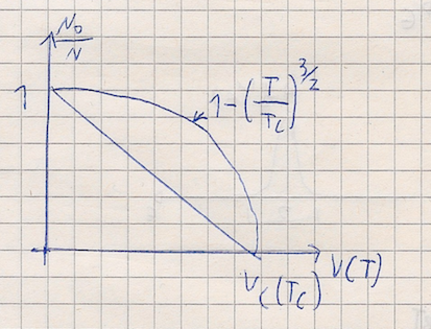
\includegraphics[width = \textwidth]{Zeichnungen/32.pdf}
  \caption{.}
  %\label{fig:Bild}
\end{figure}
\begin{align}
    \underarrow{\frac{N_0}{N}}{N_0\hat=\text{Grundzustands Besetzung}}&=
    \begin{cases}
        0 & v>v_c \\
        1-\frac{v}{v_c} \hat= 1- \left(\frac{T}{T_c}\right)^2  & (\text{für } v<v_c , T<T_c) 
    \end{cases}\\
    v_c(T) &= \frac{\lambda_T^3(T)}{\zeta\left({\frac32}\right)} \quad \lambda_T = \frac{h}{\sqrt{2\pi M \kB T}} \\
    z &= e^{\beta \mu} = 
    \begin{cases}
        1 \quad \text{für} & \frac{v}{\lambda_T^3}\leq \frac{1}{\zeta{\frac32}}\\
        \text{Lösung von } & \frac{v}{\lambda_T^3} = \frac1{g_{\frac32}(z)}
    \end{cases}
\end{align} 

%Bild33


\paragraph{Zustandsgleichung}

\begin{align}
    \frac{p}{\kB T}=\frac{1}{\lambda_T^3}g_\frac52(z) 
\end{align}

%p-T Diagramm: #caption 
%Bild34

\begin{align}
    p_c(T)&=P(v_c(T),T) \\
    &= \frac{\kB T}{\lambda_T^3} \zeta \left(\frac52 \right) = \left( \frac{M}{2 \pi \hbar^2} \right)^\frac32 \zeta \left(\frac52\right) (\kB T)^\frac52 \\
    p_c&=\text{const. für $T<T_c$ unabhängig von v}  \\
    p\leq p_c \text{für $T=$const.} \\
    \tdif{p_c}{T}&=\frac52 \left( \frac{M}{2 \pi \hbar^2} \right)^\frac32 \zeta(\frac{5}{2})(\kB T)^\frac{3}{2}=\frac52\kB \frac{\zeta\left(\frac52\right)}{\lambda_T^3}\frac{\zeta\left(\frac32 \right)T}{\zeta\left(\frac32 \right)T}\\
    & =\frac{1}{T v_c}\left[\frac{5}{2}\kB T \frac{\zeta(\frac52)}{\zeta(\frac32)}\right]=\frac{Q_L}{T \Delta v} \\
\end{align}

Form einer Clausius--Clapeyron-Gleichung
\begin{align}
    & \tdif{p_L}{T}=\frac{S_1-S_2}{v_1-v_2}=\frac{Q_L}{T \Delta v} \qquad \text{(z.B. Wasser/Eis)}\\
    \Rightarrow \text{Latente Wärme}\\
    & Q_L=\frac52 \kB T \frac{\zeta\left(\frac52\right)}{\zeta\left(\frac32\right)}
    \intertext{Annahmen}
    v(\text{Grundzustand})&=0\\
    v(\text{Rest})&=v_c \\
    \intertext{Zwei-Phasen-Modell:} 
    \intertext{\quad \quad 1. Phase: Grundzustandskondensat} 
    \intertext{\quad \quad 2. Phase: Rest aller Anregung $\epsilon>\epsilon_0=0$} 
    \intertext{$T<T_c$ Koexistenz beider Phasen} \\
\end{align}
\paragraph{Duhen-Gibbs Relation:} 
\begin{align}
    U&+pV- \mu N -TS =0 \\
    \frac{S}{N\kB}&=\frac{\beta}{N}\left[U+\frac32U-\mu N\right] \\
    &= \frac52 \beta\left(\frac{U}{N}\right)-\beta\mu \ln z \\
    &= \frac52 \frac{v}{\lambda^3_T}g_\frac{5}{2}(z)-\ln z \\
    \frac{S}{N\kB}&=
    \begin{cases}
        \frac52\frac{v}{\lambda^3_T}g_\frac52(z)-\ln z & T>T_c\\
        \frac52\frac{v}{\lambda^3_T}\zeta\left(\frac52\right)  & T<T_c
    \end{cases}
\intertext{Entropie ist an $T_c$ stetig}
    \frac{C_v}{\kB v}=\frac{1}{v\kB}\pdif{U}{T}[N,V]&=\frac52 \frac32 \frac{1}{\lambda_T^3} g_\frac{5}{2}(z)+ \frac{3}{2} \frac{T}{\lambda_T^3}g'_\frac{5}{2}(z)\pdif{z}{T}\biggr\vert_{N,v}\\
    U &= \frac32 \kB T \frac{V}{\lambda_T^3} g_\frac52 (z) \\
    \Aboxed{g'_U(z)&=\frac{1}{z}g_{n-1}(z)} \\
    g_\frac32 (z) &= \frac{\lambda_T^3}{v} \biggr\vert \pdif{}{T}[N,V] \quad \quad (N=...)^{T>T_c}\\
    g'_{\frac32}(z) \pdif{z}{T}[N,V] &= -\frac32 \frac{\lambda_T^3}{v T}\\
    \Rightarrow \pdif{z}{T}[N,V] &= -\frac32 \frac{\lambda_T^3}{v T}\frac{z}{g_\frac12(z)} \quad \quad \frac{1}{v}=\frac{N}{V} \\
    \frac{C_V}{\kB V} &= \frac{15}{4} \frac 1\lambda_T^3 g_\frac52(z) - \frac94 \frac{\cancel{T}}{\cancel{\lambda_T^3}} \frac{g_\frac32}{\cancel{Z}} \frac{\cancel{\lambda_T^3}}{\cancel{v T}} \frac{\cancel{Z}}{g_\frac12(z)} \qquad \biggr\vert \cdot \frac VN\\
    \Aboxed{\frac{C_V}{\kB N} &= \frac{15}{4} \underbrace{\frac{v}{\lambda_T^3}}_{\frac1{g_\frac52(z)} g_\frac52(z) - \frac94 \frac{g_\frac32(z)}{g_\frac12(z)}}}\\
    \lim_{z \to 1^-} \frac{1}{g_\frac12}(z) &= 0\\
    \frac{C_V}{N} \text{ist stetig an $T_C$}\\
    \frac{C_V}{\kB N}&=
    \begin{cases}
        \frac{15}{4} \frac{v}{\lambda_T^3}g_\frac52(z)-\frac94 \frac{g_\frac32(z)}{g_\frac12(z)} &T>T_c\\
        \frac{15}{4} \frac{v}{\lambda_T^3} \zeta\left(\frac52 \right)\propto T^{\frac32} & T\leq T_c
    \end{cases}
\end{align} 
%Bild35
Ehrenfest: Phasenübergang 3.Ordnung \\

Bose-Einstein-Kondensation 
\begin{enumerate}
    \item Phasenübergang 1.Ordnung in zwei Phasen(Fluid ) Moden
    \item Phasenübergang 3.Ordnung für das Gesamtsystem
\end{enumerate}
\section{Phasenübergänge}
Magnetismus 
\begin{itemize}
    \item $T>T_c$ ungeordnete Momente
    \item $T<Tc$  endliche Magnetisierung
\end{itemize}
Modell: Heisenberg Modell
\begin{align}
    H&=-\sum_{ij} J_{ji} \vec S_i \vec S_j \\
    J_{ij} &=
    \begin{cases}
        0 \quad \text{für } \Ket{\vec r_i - \vec r_j} > L_{N N}\\
        J \quad \text{für } i, j_{N N}%kein Plan
    \end{cases} \\
\Rightarrow H&=-J\sum_{\Braket{ij}} \vec S_i \vec S_j
\end{align}

\subsection{Das Ising Modell}
\begin{align}
    H &= - \tilde{J} \underbrace{\sum_{<j,i>}}_{i, j \text{ identische Nachbarn}} \vec{S}_i \vec{S}_j \qquad \text{Heisenbergmodell} \\
    \vec S_1 \vec S_2 &= \underbrace{S_{1,z} S_{2,z}}_\text{Ising-Term} + \frac12 (S_{1,+} S_{2,-} S_{1,-} S_{2,+})\\
    H_\text{Ising}&= J\sum_{\Braket{ij}} \sigma_i \sigma_j + \frac{h}{2} \sum_j (\sigma_j +  \sigma_{j+1})  \quad \sigma_{i,j}=\pm 1\\
\intertext{$1D, 2D$ lösbar; $3D$ nicht lösbar}
\intertext{Heute: 1D Ising Modell}
\intertext{$N$ Gitterplätze, Periodische Randbedingungen (Ringtopologie): $\sigma_{N+1}= \sigma_1$}
\end{align}
%%%%%Bild 36%%%%%caption: das N-te Teilchen wechselwirkt mit dem Ersten
\begin{align}
    H &= \sum_j H_j \quad ,\hat\sigma_j=2\hat S_{j,z}\\
    \hat H_j &= -J\hat\sigma_j \hat\sigma_{j+1}\\ 
    \text{Ising-Basis:} &\Ket{\sigma_1,\sigma_2,...,\sigma_j,...\sigma_N} \quad \sigma_j=\pm1\\
    \hat\sigma_j\Ket{\sigma_1,...,\sigma_j,...\sigma_N}&=\hat\sigma_i\Ket{\sigma_1,...,\sigma_j,...\sigma_N}\\
    [H_i, H_j] = 0  \qquad \Rightarrow \e^{-\beta \hat H} &= \prod_{j=1}^N \e^{-\beta \hat{H}_j} \\
    \text{Zustandssumme: } Z(T,N,h)&= \Tr\left[\e^{-\beta\hat H}\right]=\Tr\left[\prod_j \e^{-\beta H_j}\right]\\
    &=\Tr\left[\e^{-\beta\hat H_1}....\e^{-\beta\hat H_{j-1}}\underarrow{ }{\hat 1 = \sum_{\sigma_j}\Ket{\sigma_j}
    \Bra{\sigma}\hspace{2.5cm}} \e^{-\beta\hat H_{j}}\underarrow{ }{\hspace{2.5cm}\hat 1 = \sum_{\sigma_j+1}\Ket{\sigma_j}}\e^{-\beta\hat H_{j+1}}
    \e^{-\beta\hat H_{N}}\right]\\
    \text{Transfermatrix: } P_{\sigma_j \sigma_{j+1}} &= \Bra{\sigma_j} \e^{-\beta \hat{H}_j} \Ket{\sigma_{j+1}} = \e^{-\beta(-J \sigma_j \sigma_{j+1} +\frac{h}{2}(\sigma_j + \sigma_{j+1})} \\
\end{align}
\begin{align}
    2 \times 2-\text{Matrix:} \quad P &= 
    \begin{pmatrix}
        \e^{\beta(J-h)} & \e^{-\beta J} \\
        \e^{-\beta J} & \e^{\beta(J+h)} \\
    \end{pmatrix}\\
    Z(T,N,h)&=\Tr[P^N]=\lambda_+^N+\lambda_-^N \\
    \lambda_\pm &\quad \text{Eigenwerte von } \tensor{P}\\
    \tensor P &= \tensor U \underbrace{
    \begin{pmatrix}
        \lambda_+ & 0\\
        0   & \lambda_-\\
    \end{pmatrix}}_{\tensor D_p}\tensor U ^{-1} \\
    \tensor P^N &= \left[ \tensor U \tensor D_P \tensor U^-\right]^N = \tensor U \tensor D_P^N \tensor U^{-1}\\
    x&=\e^{\beta J}, \quad y=\e^{-\beta h} \\
    O&=\lvert \tensor P -\lambda \tensor 1 \rvert=
    \begin{vmatrix} 
        xy-\lambda & \frac{1}{x} \\
        \frac{1}{x}  & \frac{x}{y}-\lambda\\
    \end{vmatrix} \\
    &=(xy-\lambda)(\frac{x}{y}-\lambda)-\frac{1}{x^2}=\lambda^2-\lambda x(\underarrow{y}{2\cosh(\beta h)}+\frac1y)+x^2-\frac{y}{x^2}=0\\
\end{align}
\begin{align}    
    y + \frac{1}{y} &= \e^{-\beta H} + \e^{\beta H} = 2 \cosh(\beta h) \\
    x^2 - \frac{1}{x^2} &= \e^{2 \beta J} - \e^{2 \beta J} = \sinh(2 \beta J) \\
    \lambda_{\pm} &= x \cosh(\beta h) \pm \sqrt{x^2 \cosh^2(\beta h) - 2\sinh(2\beta J) } \\
    &= \e^{\beta J} \left[\cosh(\beta h) \pm \sqrt{\cosh^2(\beta h) - 2\e^{-2\beta J} \sinh(2\beta J))} \right] \\
    \lambda_{+} &> \lambda_{-} \\
    \frac{1}{N}\Phi(T,N,h)&=-\frac{\kB T}{N} \ln(\underbrace{\lambda_+^N+\lambda_-^N}_{\lambda_+^N\left(1+\left(\frac{\lambda_-}{\lambda_+}\right)^N\right)})\\
    &=-\kB T\ln\lambda_+ -\frac{\kB T}{N} \ln\left(1+\underbrace{\left(\frac{\lambda_-}{\lambda_+}\right)^N}_{<1,\to 0,N\to \infty}\right)\\
    \lim_{N\to \infty} \frac 1N \Phi (T, N, h) &= -\kB T \ln(\lambda_+)\\
    &= -J - \kB T \ln\left[\cosh(\beta h) + \sqrt{\cosh^2(\beta h) - 2 \e^{-2\beta J} \sinh(2\beta J) }\right]\\
    m &= \frac{M}{N} = - \frac{1}{N} \pdif{\Phi}{h}[T, N] \\
    &= \cancel{\kB T} \frac{\cancel{\beta} \sinh(\beta h)}{\cancel{\cosh(\beta h) + \sqrt{...}}} \left[\underbrace{1+\frac{1}{\cancel{2}} \frac{\cancel{2} \cosh(\beta h)}{\sqrt{...}}}_{\cancel{\frac{\sqrt{...}+\cosh(\beta h)}{\sqrt{...}}}} \right] \\
    &= \frac{\sinh(\beta h)}{\sqrt{\cosh^2(\beta h)  - 2 \e^{-2 \beta J} \sinh(2 \beta J)}} \\
    \lim_{h\to 0}m(h) &= 0 \Rightarrow m\approx h \Rightarrow m=\chi h \qquad (\chi:\text{mag. Suszeptibilität})\\
    &\text{Magnetische Phase: } \lim{h \to 0} m(h) = m_0 \pm 0 \\&(\text{nicht im $1D$ Ising-Modell bei $T>0$})\\
    \chi&=\pdif{m}{h}[h=0]
\intertext{2 Strategien in der Theorie der Phasenübergänge}    
\end{align}

\begin{enumerate}
    \item Symmetriebrechung durch ein externes Feld $(h)$
    \item Berechne $\chi(h=0)$
\end{enumerate}

\begin{align}
    \chi(T)\biggr\vert_{h\to 0}&=\pdif{m}{h}[h\to 0] =\beta\left[\frac{\cosh(\beta h)}{\sqrt{...}}-\frac12 \frac{\sinh(\beta h)^2(\to 0)}{\sqrt{..}^3}\right]\biggr\vert_{h\to 0} \\
    &= \beta \frac{1}{\sqrt{\cancel{1} - \cancel{2} \underbrace{\e^{-2\beta J} \frac{1}{\cancel{2}} (\e^{2 \beta J} -\e^{-2\beta J)}}_{1-\e^{-4\beta J}}}} = \beta \e^{2 \beta J} \\
\intertext{1. Fall: nicht wechselwirkende Spins: $J=0$}
    \chi(T)&=\frac{1}{\beta} =\frac{1}{\kB T} \propto \frac{1}{T} \quad \text{Curie-Gesetz für ein freies mag. Moment}\\
    \chi(T)&=\frac{1}{\kB T}\e^{2\beta J}\text{steigt stärker an als das Curie-Gesetz für $J\neq 0$} \\
    \lim_{T \to \infty} &\to \infty \\
    \text{Entropie pro Gitterplatz:} &\quad \frac{S}{N}=-\frac{1}{N}\pdif{}{T}\Phi \text{ stetig}\\
    \text{Spezifische Wärme:} &\quad  C_V = T \pdif{S}{T} \text{stetig für $T>0$}\\
\intertext{2D-Ising-Modell: kritische Temperatur $ T_C > 0; T_C \approx J$}
\end{align}

\subsection{Theorie des mittleren Feldes}
\begin{align}
    H &= -J \sum_{<i,j>} \vec{S}_i \vec{S}_j \qquad \text{Heisenberg-Modell}\\
    &=J\sum_i \vec S(-J)\underbrace{\sum_{<j,\text{max}>} \vec{S}_j}_{\vec B_i^{\text{eff}}}
\end{align}
%Bild 37 caption: Spins koppeln nur mit nächsten Nachbarn
\begin{align}
    F[\hat \rho] &= \Braket{\hat H} - T S[\hat \rho] = \Tr[\rho \hat H] + \kB T \Tr[\hat \rho \ln \hat \rho]\\
\intertext{ist für das Heisenberg Modell nicht exakt lösbar für $D>1$ }
    \hat\rho_\text{th} &= \frac{\e^{\beta \hat H}}{Z}; \qquad Z = \Tr [\e^{-\beta \hat H}]\\
    F[\hat \rho] &\geq F[\hat \rho_\text{th}]\\
\intertext{Näherung:}
    \rho_\text{th}\to \hat \rho_\text{trial}(\lambda_1,\lambda_2,..\lambda_N...)
\end{align}
\begin{enumerate}
    \item Einschränkung im Raum der Dichteoperatoren
    \item $F[\rho_\text{trial}(\lambda_i)] \geq F[\rho_\text{th}]$ \\
    Variationsansatz: \\
    \begin{align}
        \pdif{F}{\lambda_i} = 0 \ \forall \lambda_i
    \end{align}
\end{enumerate}
Frage: Wie wählen wir $\hat \rho_\text{trial}$?
\begin{align}
    \text{Antwort: } \rho_\text{trial} &= \frac{\e^{-\beta\hat H_\text{eff}}}{Z_\text{MF}}, \quad Z_\text{MF} = \Tr\left[\e^{-\beta\hat H_\text{eff}}\right]
    H_\text{eff}=-\sum_j \vec S_i \vec X_i\\
    [\vec X_i]: &\qquad \text{Energie, klassischer Vektor}
\end{align}
%Bild 38 caption: Spin in einem Magnetfeld $\vec x_i$
\begin{align}
    F[\hat \rho_\text{MF}(\{\vec X_i\})]&=F(\{\vec X_i\})=\Tr[\rho_\text{MF} \hat H]+\kB T \Tr[\rho_\text{MF}(-\beta \hat H_\text{eff} -\ln Z_\text{MF})]\\
    &=\Tr[\rho_\text{MF}(\underarrow{H-H_\text{eff}}{\text{Korrekturterm}\ \Braket{\Delta H}})]-\frac{1}{\beta} \ln Z_\text{MF}
\intertext{Zustandssumme:}
    Z_\text{MF}&=\Tr[\e^{-\beta H_\text{eff}}]=\Tr[\e^{\sum_i \beta \vec S_i \vec X_i}]=\prod_{i=1}^N \Tr[\e^{\beta \vec S_i \vec X_i}]=\prod_i Z_i\\
    \Tr\left[\hat \rho_\text{MF} \hat H_\text{eff}\right] &= - \sum_j \Tr\left[\rho_\text{MF}\vec S_i \vec X_i\right] = -\sum_j \Braket{\vec S_j} \vec X_j\\
    \Tr\left[ \rho_\text{MF} \hat H \right] &= - J \sum_{ \Braket{j, i}} \Tr[\rho_\text{MF} \vec S_i \vec S_j]
    = - J \sum_{\Braket{j, i}} \Braket{\vec S_i} \Braket{S_j}
\end{align}

\begin{align}
    F(\{\vec{x}_i\}) &= - \sum_{i} \Braket{\vec{S}_n} \left( \left(\sum_{j \in NN(n)} J \Braket{\vec{S}_j} \right)  - \vec{x}_n \right) - \frac1{\beta} \ln(Z_\text{MF}) \\
    0 &= \pdif{F}{X_{i,\underarrow{\alpha}{\alpha=x,y,z}}}
    = \cancel{\Braket{S_{i,\alpha}}} - \sum_n \vec{X}_n \pdif{\Braket{\vec S_n }}{X_{i,\alpha}} - J 
    \underbrace{
        \pdif{}{X_{i,\alpha}} \left(\sum_{\Braket{n,m}} \Braket{\vec S_n} \Braket{\vec S_m}\right)
    }_{
        \underbrace{
            \sum_{\Braket{n,m}} \pdif{\Braket{\vec S_n}} {x_{i,\alpha}} \Braket{\vec S_m} + \Braket{\vec S_n} \pdif{\Braket{\vec S_m}}{x_{i,\alpha}}
        }_{
            2\sum_{\Braket{n,m}} \Braket{S_n} \pdif{\Braket{\vec S_m}}{x_{i,\alpha}}
        }
    } \\
    &-\frac{1}{\cancel{\beta}}\underbrace{
        \cancel{\frac{1}{Z_\text{MF}}\cancel{\beta} \Tr[S_{i,\alpha}\e^{\beta\vec S_{i}\vec X_{i} }]\prod_{n\neq i} Z_i}
    }_{
        \Braket{\hat S_{i,\alpha}}
    }
    \\&= \sum_n \left(\vec X_n - 2 J \sum_{m \in NN(n)} \Braket{\vec S_m}\right) \underarrow{\pdif{\Braket{\vec S_n}}{X_{i, \alpha}}}{\neq 0} = 0 \\
    \Rightarrow \Aboxed{\vec X_n &= 2 J \sum_{m \in NN(n)} \Braket{\vec S_m}} \qquad \text{MF Selbstkonsistenzgleichung}\\
    \vec X_n &= 0 \Rightarrow \Braket{\vec S_j} = 0 \quad \text{ist immer eine Lösung }
\intertext{paramagnetische Phase}
\end{align}
Hier: $J > $: Ferromagnetismus
\begin{itemize}
    \item Alle Spins richten sich in z-Richtung aus
    \item Translationsinvariante Lösung
\end{itemize}

\begin{align}
    \vec{x}_n \to \vec{x} &\neq x \vec e_z\\
    \text{SCG: }\ x &=2 p J\Braket{S_z}  \quad; p = \text{\# nächste Nachbarn} = 2d\\  
    Z_i &= Z=\Tr[\e^{\beta S_z x}]=\sum_{m=-L}^L \e^{\beta m x} \\
    &= \e^{\beta L x} \sum_{m=0}^{2 L} e^{-\beta m x}=\e^{\beta L x} \frac{\e^{-\beta(2L+1)x}-1}{\e^{-\beta x}-1}\\
    &= \frac{\e^{-\beta (L+1)x} - \e^{\cancel{-}\beta L x}}{\e^{-\beta x} - 1 } \frac{\e^{\beta \frac L2 x}}{\e^{\beta \frac L2 x}} = \frac{\sinh \left(\left(L + \frac12\right)\beta x\right)}{\sinh \left(\frac L2 \beta x\right)}\\
    \Braket{S_z} &= \frac 1Z \Tr\left[\hat S_z \e^{\beta S_z x}\right] = \frac 1\beta \pdif{}{x} (\ln(Z)) \\
    &= (L + \frac12) \coth\left(\beta \left(L + \frac12\right)x\right) - \frac L2 \coth\left( \frac{\beta x}{2}\right)\\
\intertext{wir verwenden die Identität $\equiv L B_L(\beta L x)$}
    \pdif{}{x}\ln(\sinh(\alpha x)) &= \alpha \frac{\cosh(\alpha x)}{\sinh(\alpha x)}
\intertext{Brillouin-Funktion}
    B_L(x)&=\frac{2L+1}{2L} \coth(\frac{2L+1}{2L}x)-\frac{1}{2L}\coth(\frac{1}{2L}x)
\intertext{Spin $\frac12$}
    B_\frac12(x) &= 2 \coth(2 x) - \coth(x)
    = 2\underbrace{\frac{\e^{2x}+\e^{-2x}}{\e^{2x}-\e^{-2x}}}_{(\e^{x-\e^{-x}})(\e^{x}+\e^{-x})} -\frac{(\e^{x}+\e^{-x})^2}{(\e^{x}-\e^{-x})(\e^{x}+\e^{-x})} \\
    &= \frac{\overbrace{\cancel{2} (\e^{2x} + \e^{-2x}) - (\cancel{\e^{2x} + \e^{-2x}} + 2)}^{4 \sinh^2(x)}}{(+) (-)} \\
    &=\frac{\cancel{4}\sinh^{\cancel{2}}(x)}{\cancel{4}\cancel{\sinh(x)}\cosh(x)}=\tanh{x}\\
    \Aboxed{x &=  pJ \tanh(\beta \frac x2)}
\end{align} 

\begin{align}
    \hat \rho_\text{MF} &= \frac 1Z_\text{MF} \e^{-\beta \hat H_\text{eff}}; \qquad H_\text{eff} = -\sum_j \vec S_j \vec X_j\\
    \vec X_j &= g \mu_B \vec B_j^\text{eff}\\
    \Braket{S_Z} &= \frac LL \left(L + \frac12 \right) \coth \left(\beta \left(l + \frac12 \right) X \frac LL \right) - \frac12 \frac LL \coth \left(\beta \frac x2 \frac LL \right)\\
    &= L B_L(\beta Lx)\\
    \Aboxed{X &= 2pJ\Braket{S_z}} \quad \text{für} \quad X_i = X\\
    B_L{x} &= \frac{2L+1}{2L} \coth(\frac{2L+1}{2L} x) - \frac{1}{2L}\coth(\frac{x}{2L}) \\
\end{align}
%Bild 39 caption:
%Bild 40 caption:
\begin{enumerate}[i]
    \item Paramagnetische Phase (PM)
    \begin{itemize}
        \item $\beta$ < $\beta_c$ \quad $T>T_c$ 
        \item $\Braket{S_z} = 0$ \quad $X=0$
    \end{itemize}
    \item Ferromagnetische Phase (FM)
    \begin{itemize}
        \item $\beta$ > $\beta_c$ \quad $T<T_c$ 
        \item $\Braket{S_z} > 0$ \quad $X>0$
    \end{itemize}    
\end{enumerate}

\begin{align}
    \intertext{Spinsuszeptibilität (PM):}
    \increment H &= H_1 = - \sum_j \vec{S}_j (g \mu_\text{B} \vec{B}_\text{ex}) = - \sum_j \vec{S}_j \vec{x}_\text{ex} \\
    \text{mit: } \quad \alpha, \beta &= x, y, z\\
    X_{\alpha, \beta} &= \pdif{M_\alpha}{B_\beta} = \pdif{(g \mu_B \Braket{S_\alpha})}{B_\beta} \frac{(g \mu_B)}{(g \mu_B)} = (g \mu_B)^2 \pdif{\Braket{S_\alpha}}{X_\alpha} \delta_{\alpha, \beta}\\
    \chi_{\alpha \beta} &= \delta_{\alpha \beta} (g \mu_\text{B})^2 \beta L^2 B_L'(\beta L x)\vert_{x \to 0} \\
\intertext{Taylor-Entwicklung}
    \coth{x} &= \frac{1}{x} + \frac{x}{3} - \frac{x^3}{45} + \mathcal O(x^5) \\
    B_L(x) &= ... = \frac{L+1}{3L} x - \frac{x^3}{45} \frac{(2L+1)^4-1}{(2L)^4} + \mathcal O(x^5) \\
    \Chi_{\alpha, \beta} &= \delta_{\alpha, \beta} (g \mu_B )^2 \beta L^{\cancel{2}} \frac{(L + 1)}{3\cancel{L}} = \delta_{\alpha, \beta} \underbrace{(g\mu_B)^2 \frac{L(L+1)}{3} \frac{1}{\kB T}}_{\text{Curie-Gesetz}}
\end{align}

\paragraph{Selbstkonsistente Lösung der Mean-Field-Gleichung:}


\begin{align}
    \Braket{S_Z} &= L B_L (\beta L x ) \stackrel{x \to 0}{\approx} \cancel{L} \frac{(L + 1)}{3 \cancel{L}} (\beta L X) + \mathcal O(x^3)\\ 
    &\text{Mean-Field-Gl.} \quad X \to 0 \\
    X &= 2P J \Braket{S_z} \approx 2P J \frac{L(L+1)}{3} \beta X\\
    \Rightarrow \Aboxed{\kB T_\text{C} &= 2pJ \frac{L(l+1)}{3}} \\ 
    x &= 0 \qquad \text{für: } \quad T_C < T\\
    x &\neq 0 \qquad \text{für: } \quad T < T_C
\end{align}

Frage: 
\begin{itemize}
    \item $x>0$: Thermodynamisch stabil, $F(x) < F(0)$?
    \item Analytische Form von $X(T)$ 
\end{itemize}


\begin{align}
    F(x) &= - \sum_j \Braket{\vec S_j} \sum_{m \in NN(j)} J \Braket{\vec S_m} - \underarrow{\vec X_j}{X \vec e_z}) - \frac 1\beta \ln(Z_\text{AF}) \\
    &(NN(j) = \text{\enquote{nearest neighbours of $j$}})\\  
    &= -N \frac{X}{2pJ} \left( \cancel{p} \frac{\cancel{J} X}{2 \cancel{pJ}} - X \right) - N \ln \left(\frac{\sinh((L+\frac{1}{2}) \beta x)}{\sinh(\beta \frac{x}{2})} \right)  \qquad \Aboxed{ \Braket{S_z} = \frac{X}{2PJ}} \\
    &= N \left[ \frac{X^2}{4 p J} - \frac 1\beta \ln(...)\right]
\end{align}

\begin{align}
\intertext{Nebenrechnung}
    \sinh(y) &= y + \frac{y^3}{3!} + \mathcal O(y^5)\\
    \ln(1 + y) &= y - \frac{y^2}{2} + \mathcal O(y^3)
\end{align}

\begin{align}
    \ln \left( \frac{\sinh(ax)}{\sinh(bx)} \right) &\approx \ln \left( \frac{ ax + \frac{1}{6} (ax)^3 +...}{ bx + \frac{1}{6} (bx)^3 +...} \right)\\
    &= \ln \left(\frac ab \frac{1 + \frac16 (ax)^2 ...}{1 + \frac16(bx)^2 ...} \right) = \ln \left( \frac{a}{b} \right) + \left(\frac{(ax)^2}{6} - \frac{(bx)^2}{6} \right) + \mathcal O(x^4) \\
    &= \ln \left(\frac ab \right) + \frac{x^2}{6} (a^2 - b^2) + \mathcal O(x^4)\\
    \text{mit:} \quad a &= \beta\left(L + \frac12 \right) \quad b = \frac \beta2\\  
    \frac{F(x)}{N} &\approx \frac{X^2}{4pJ} - \frac1{\cancel{\beta}} \left[ \ln (2L+1) + \frac{x^2}{6} \frac{\beta^{\cancel{2}}}{\cancel{4}} [\underbrace{(2L+1)^2-1}_{2L(2L+1) = \cancel{4}L(L+1)}]+...\right] \\
    &\approx  T \underbrace{\kB  \ln (2L + 1)}_{\text{Entropie pro Spin}} + \frac{X^2}{4 pJ} - \beta \frac{L(L + 1)}{6} x^2\\
    F &= U - TS
\end{align}

\begin{align}
    \kB T_\text{C} &= 2p J \frac{L (L+1)}{3}\\
    \beta_\text{C} &= \frac{3}{2pJ L(L+1)} \Rightarrow \frac{1}{4pJ} = \frac{L(L+1)}{6} \beta_C\\
    \frac{F(x)}{N} &\cong -\kB T \ln (2L+1) + \underbrace{x^2\left(\beta_\text{C} \frac{L(L+1)}{6} - \beta \frac{L(L+1)}{6} \right)}_{ x^2 \frac{L(L+1)}{6} \beta_\text{C}\underbrace{\left(1- \frac{\beta}{\beta_C} \right)}_{1-\frac{T_\text{C}}{T}}} \\
    \text{Für: } T < T_C \quad &\hat = \quad \beta > \beta_C\\
    \text{gilt: } (1- \frac{\beta}{\beta_C}) &< 0\\
    \Rightarrow F(x) - F(0) &< 0 \quad \text{für} \quad T < T_\text{C} \\
\intertext{$\Rightarrow$ thermodynamisch stabil} \\
    (ii) \to X(T) &= ? \\
    \Braket{S_z} &= \frac{L(L+1)}{J} \beta X \left( 1 - \underarrow{\frac{L^2 + L + \frac12 }{15}}{Y^2} (\beta x)^2 + \cdots \right)\\
    X &= \underbrace{2pJ \frac{L(L+1)}{3}}_{\frac{1}{\beta_\text{C}}} \beta X (1 - \gamma ^2 (\beta x)^2) \\
    \cancel{X} &\approx \frac{\beta}{\beta_C} \cancel{X} ( 1 - \gamma^2 (\beta X )^2 )\\
    \frac{\beta_\text{C}}{\beta} &= (1 - \gamma^2 (\beta X)^2)\\
    \gamma^2 (\beta x)^2 &= 1 - \frac{\beta_\text{C}}{\beta} = 1 - \frac{T}{T_\text{C}} = \frac{T_\text{C} -T}{T_\text{C}} = t \quad \text{reduzierte Temperatur} \\
    X &= \frac{\kB T_\text{C}}{\gamma} t^\frac12  = A t^\beta\\
\intertext{$\beta$: kritischer Exponent des Ordnungsparameters \rightarrow MF-Theorie $\beta = \frac{1}{2}$}
\end{align}
%Bild41 caption:

\subsection{Landau-Theorie der Phasenübergänge}
Räumliche  Mittelung:
%Bild42 caption: Mittelung
Allgmeiner: $m(\vec r)$ 
\begin{align}
    l:\text{mikroskopisch groß aber makroskopisch klein}
\intertext{Vereinfachung}
\end{align}
 \begin{enumerate}
    \item Vernachlässigung von Räumfluktuationen:$m(\vec{r},T) \to m(T)$ 
    \item M sei statisch und verschwindet bei $T=T_c$
        \begin{align}
            m(T>T_c) &= 0\\
            m(T<T_c) &\neq 0
        \end{align}
    \item $F(m,T)$ wird als Taylorreihe in m entwickelt
\end{enumerate}
\begin{align}
    \intertext{nahe $T_c$ gilt:}
    F(m,H) &\tilde{=} T_0+\frac 12 r_0(T)m^2+U_0 m^4 - m \underarrow{H}{\text{externes Magnetfeld}}
\intertext{Für $H=0$}
%Bild43 caption: für H=0
\intertext{Minimierung der Freien Energie}
    \pdif{F}{m}&= r_0(T) m+4 U_0 m^3 -H=0
\intertext{Für $H=0 \Rightarrow$ zwei Lösungen}
\end{align}
\begin{itemize}
    \item triviale Lösung $m=0$
    \item \begin{align}
            r_0(T) + 4 k_0 m^2 &= 0\\
            m^2 = - \frac{r_0(T)}{4 k_0} \Rightarrow m_\pm &= \pm \sqrt{\frac{|r_0(T)|}{4k_0}}
          \end{align}
\end{itemize}
\begin{align}
\intertext{Entwicklung von $r(T)$ um $T_c$}
    r_0(T) &\approx \underbrace{r_0(T_c)}_{=0}+\overline{a}_0(T-T_c)= \underline{\overline{a}}_0 T_c  \frac{T-T_c}{T_c}=a_0 t\\
    t &= \frac{T-T_c}{T_c} \text{reduzierte Temperatur}\\
    \Rightarrow \bar{M} &= \sqrt{- \frac{a_0}{4 k_0} t} \underarrow{=}{t<0} \sqrt{\frac{a_0}{4 k_0} |t|} \propto |t|^{frac12} = |t|^{\beta} 
\intertext{kritischer Exponent $\beta =\frac 12$}
    F(\overline{m})-F_0&\underarrow{=}{t<0} \frac 12 a_0 t \frac{a_0}{4U_0}\lvert t\rvert+\cancel{U_0}\frac{a_0^2}{16 U_0^{\cancel{2}}}\lvert t\rvert^2=-\frac{1}{16} \frac{a_0^2}{U_0}\lvert t\rvert^2 < 0\\  
    t|t| &= -|t|^2\\
\intertext{Suszeptibilität}
    \Chi &= \pdif{m}{H}[H\to 0]\\
    r_0(T) \underbrace{\pdif{m}{H}}_{\Chi} + 4k_0 3 m^2 \underbrace{\pdif{m}{H}}_{\Chi} -1 &= 0\\
    \Rightarrow \Aboxed{\chi &= \frac{1}{r_0(T) + 12 k_0 m^2}} \quad \text{mit } m = \overline m
\end{align}
\begin{enumerate}
    \item   \begin{align}
            T>T_c \Rightarrow \overline{m}=0\\
            \Chi=\frac{1}{r_0(T)}=\frac{1}{a_0} t^{-1}=\frac{1}{a_0}\lvert t\rvert^{-1}
            \end{align}
            $\chi$ divergiert an $T_c$
            \begin{align}
                \Chi \propto \lvert t \rvert^{-\gamma}\Rightarrow \gamma = 1
            \end{align}
    \item $T< T_C (t < 0)$
            \begin{align}
                \text{Nenner: } r_0 + 12 U_0 \left(-\frac{r_0}{4 k_0}\right) &= - 2r_0 = - 2a_0 t = 2 a_0 |t|\\
                \chi &= \frac{1}{2a_0 \lvert t \rvert} \propto \lvert t\rvert^{-1}\\
            \intertext{Phasenübergang 2. Ordnung (kontinuierlicher Phasenübergang)}
            \intertext{Spontane Symmetrie Berechung}
                \text{Spezialfall: } r_0(T) &= 0\\
                4 k_0 m^3 - H &= 0\\
                m = \left(\frac{1}{4 k_0}\right)^{\frac13} H^\frac13 \propto H^\frac1\delta \Rightarrow \delta &= 3
            \end{align}
\end{enumerate}
Spezifische Wärme
\begin{align}
    C_V &= T \pdif{S}{T}\\
    \Delta C_v &= T\pdif{\Delta S}{T}\\
    \Delta S &= - \pdif{\Delta F}{T}=\pdif{}{T} \left(\frac{a_0^2}{16U_0} \frac{(T-T_c)^2}{T_c^2} \right)\\
    &=\frac{a_0^2}{8 U_0} \frac{1}{T_c^2}(T-T_c)
\intertext{$\Rightarrow S$  ist an $T_c$ stetig, da $\Delta S(T_c)=0$}
    T\pdif{\Delta S}{T} &= \frac{a_0^2}{8 U_0}\frac{T}{T_c}>0
\end{align}
%Bild 44 caption: $C_V$ hat einen Sprung bei $T_C$
\begin{align}
    C_v\propto &\lvert t\rvert^{-\alpha}\\
    \text{Hier } \alpha &=0 \lvert\text{keine Divergenz um $C_v(T\to T_c)$}\\
\intertext{Ausblick:}
    F[m(\vec{r})] &= \int \dif^d r \left(\frac 12 r_0(T)m(\vec r)^2+U_0 m(\vec r)^2+\frac 12 \lvert \nabla m \rvert^2-hm(\vec) \right)\\
    F &= -\frac 1\beta \ln(Z) \rightarrow Z = \int D[m] \e^{-\beta F [m(r)]}\\
    Z &=\Tr[e^{-\beta H}]
\end{align}

\subsection{Das Theorem von Mermin und Wagner (1966)}

In $1D$ und $2D$ kann es im isotropen Heisenbergmodell keine spontane Magnetisierung geben. 2($T_C > 0$ nicht möglich.)
Verallgemeinerung auf andere Probleme mit kon. Symmetriebrechung, z.B. Supraleitung um Kristallisation.
\begin{align}
    \intertext{Thermodynamischer Limes}
    \overline{O}=\lim_{V\to\infty,N\to \infty} \frac{1}{V} \Braket{\hat O},   \quad \quad \text{$\hat O$ extensiv}
\end{align}

\paragraph{Theorem von Mermin und Wagner}
In 1D und 2D gibt es keine spontane Symmetriebrechung einer \emph{kontinuierlichen} Symmetrie.
Sei $\hat\Gamma_s^i$ ein Generator der Symmetrietrafo (Beispiel $\vec{S}(\vec{L})$ erzeugen eine Drehung)
\begin{align}
    [\hat H,\hat \Gamma_S^i]&=0\\
\intertext{falls: } 
    \hat C_i&=[\hat A ,\hat \Gamma] \qquad (\text{Beispiel }\ S_z=i\hbar[S_x,S_y])
\intertext{dann gilt:}
    \Braket{\hat C_i} &= \Braket{[A, \Gamma_S^i]} = \Tr [\underarrow{\hat \rho}{\rho = \frac{\e^{-\beta H}}{Z} \Rightarrow [\rho, \Gamma_S^i = 0]} (\hat A \Gamma_s^i - \Gamma_S^i \hat A)] = 0
\intertext{Wir brechen die Symmetrie explizit:}
    H_g &= H-g\hat V, \qquad [\hat V,\Gamma_s]\neq 0\\
    \overline{O}_q&=\lim_{g \to 0}\lim_{\substack{V\to 0 \\ (N\to 0)}} \Tr\left[ \frac{\e^{-\beta H_g}}{Z_q} \hat O\right]
\intertext{Heisenbergmodell}
    H_b&=\underbrace{-\sum_{ij} J_{ij} \vec{S}_i \vec{S}_j}_{H} -b\sum_j S_j^z \e^{-i\vec{\mathcal K} \vec R_j}
\intertext{Wähle $\vec \mathcal K$:}
    \text{Ferromagnetisch: } \vec \mathcal K &= 0\\
    \text{Anti-Ferromagnetisch: } \e^{i \vec \mathcal K \vec R_{j}} &=
    \begin{cases}
        1 & \text{für alle $\vec R_j \in$ Untergitter A}\\
        -1 & \text{für alle $\vec R_j \in$ Untergitter B}   
    \end{cases}
\intertext{Ordungsparameter}
    S_z&=\frac1N \sum_j \Braket{S_j^z}\e^{i\vec \mathcal K \vec R_j} \\
    \text{Frage:} \lim_{b \to 0} S_z(n) &\neq 0?
\intertext{Ausgangspunkt ist die Bogoliubov Ungleichung (1962)}
    \frac 12 \Braket{\{\hat A, \hat A^\dagger \}} \Braket{[[\hat C,\hat H],C^\dagger ]} &\geq \lvert\Braket{[C,A]} \rvert^2\\
    \Braket{O} &= \Tr[\rho \hat O]
\intertext{Schwarzsche Ungleichung}
    \lvert(A|B)\rvert^2 &\leq (A|A) \cdot (B|B)\\
\intertext{Skalarprodukt}
    (\hat A|\hat B) &= \sum_{E_n \neq E_m} \Braket{n|\hat A^\dagger|m} \Braket{m|B|n} \frac{W_m - W_n}{E_n - E_m}\\
    W_{n(m)} &= \frac{\e^{-\beta E_{n(m)}}}{Z}\\
    \text{Bogoliubov: } B&=[C^\dagger,H]\\
    \vec S (\vec K)&=\sum_j\e^{i\vec \mathcal K R_j} \lvert \vec S_j=\frac{1}{N} \sum_{\vec k} \vec S(\vec K) e^{î\vec K R_j}\\
    (S^\pm(\vec K)=...)
\intertext{wir verwenden:}
\end{align}
\begin{align}
    \hat C &= \hat S^+ (\vec K)\\
    \hat A &= \hat S^- (-\vec k-\mathcal K) \\
    [\hat C, \hat A] &= [S^+(\vec k), S^-(-\vec k + \vec \mathcal K)] = 2 \hbar \sum_j S_j^z \e^{\symup i \mathcal K \vec R_j} \cdot \frac NN \\
    \lvert \Braket{[C, A]} \rvert^2 &= 4 \hbar^2 N^2 \lvert S_Z \rvert^2\\
    \Braket{\{A(\vec k),\hat A^\dagger( \vec k) \}}&=... \leq 2N \sum_i \Braket{\vec S_i^2} \\ &=2N^2\underarrow{\hbar^2}{\text{Spinlänge}} S(S+1) \qquad  
    \left(\vec S_1 \vec S_2=\vec S^z_1 \vec S^z_1+\frac 12 (\vec S^+_1 \vec S^-_2- \vec S^-_1 \vec S^+_2)\right) \\
    \tdif{}{t} \hat C &= \frac{\symup i}{\hbar} [\hat C, H] \qquad \text{Fluktuationen von } \hat C \\
    ..........
\end{align}

\begin{align}
    \Aboxed{\frac{\lvert S_z\rvert^2}{\hbar^2} \frac 1N \sum_{\vec k} \frac{1}{b S_z +\hbar^2 S(S+1) Q k^2 } &\leq \frac{1}{\kB T} S(S+1)}\\
    Q = \sum_n J_\text{on} (\vec R_n)^2 &< \infty \\
\intertext{muss endlich sein. D.h. $J_{nm}$ muss schnell genug abfallen}
    \overline{\omega}=\hbar^2 S(S+1)Q k_0^2
\intertext{$k_0:$ Radius der Größeren Kugel die in die erste  Brillouin-Zone passt}
    \frac{|S_z|^2}{\hbar ^2}\frac{V}{N}\int_{1.BZ} \frac{\dif^d k }{(2\pi)^2}\frac{1}{(...)} &\leq \beta S(S+1)   \biggr\vert \substack{V\to \infty \\N\to \infty} \text{mit} \frac{V}{N}=v\\
    \frac{|S_z|^2}{\hbar ^2} v \frac{O_d}{(2\pi)^d} \int_0^{k_0} \dif k \frac{k^{d-1}}{|b S_z|+\overline{\omega}\left(\frac{k}{k_0}\right)^2} &\leq \beta S(S+1)\\
    \frac{1}{|b S_z|} \int_0^{k_0} \dif k \frac{k^{d-1}}{1+\frac{\overline{\omega}}{|b S_z|}\left(\frac{k}{k_0}\right)^2} & =\frac{1}{|b S_z|} \left(\frac{b S_z k_0^2}{\overline{\omega}}\right)^{\frac{d}{2}} \int_0^{x_0} \dif x \frac{x^{d-1}}{1+x^2} \\
    &=|b S_z|^{\frac{d-2}{2}} \frac{k_0^d}{(\overline{\omega})^{\frac{d}{2}}} \int_0^{x_0} \dif x \frac{x^{d-1}}{1+x^2}\\
    x^2 &= \left(\frac{\overline \omega}{b S_z}\right) \left(\frac{k}{k_0}\right)^2
\end{align}

\begin{itemize}
    \item 1D: 
        \begin{align}
            \int_0^{x_0} \dif x \frac{1}{1 + x^2} = \arctan(x_0)
        \end{align}
    \item 2D
        \begin{align}
            \frac12 \int_0^{x_0} \frac{2x}{1+x^2} = \frac12 \ln(1+x_0^2)
        \end{align}
    \item 3D:
        \begin{align}
            \int_0^{x_0} \dif x \frac{x^2 +1 -1}{1 + x^2} = x_0 - \arctan (x_0)
        \end{align}
\end{itemize}

\paragraph{Eine Raumdimension}
\begin{align}
    \beta S(S+1) &\geq v \frac{|S_z|^2}{\hbar^2} \frac{1}{2 \pi} \frac{k_0}{\sqrt{\beta S_z \overline{\omega}}} \arctan \left( \sqrt{\frac{\overline \omega}{\beta S_z}}\right) \\
    \text{Jetzt } b\to 0 \qquad  \arctan(x\to\infty) &= \frac{\pi}{2}\\
    S_z &\leq \mathcal C \frac{b^\frac13}{T^\frac25}\\
    \lim_{b\to0} S_z &= 0 \\
\end{align}
\paragraph{Zwei Raumdimension}   
\begin{align}
    S_z^2 < C \frac{1}{T} \frac{1}{\ln(1+\frac{\overline{\omega}}{b S_z})}\\
    |S_z|< \frac{C'}{\sqrt{|T\ln(b)|}}\\
    \lim_{b \to 0} S_z^{2D}(b)=0
\end{align}
 
Fin.
    
    
%z 432 ist nocj kapiutt :D

\end{document}